\RequirePackage{pdfmanagement-testphase}
\DeclareDocumentMetadata{}
\documentclass[a3paper,openany,twoside]{book}

\newcommand{\PATH}{../../../../}

\usepackage{\PATH templates/utilities/image-db}
\usepackage{\PATH templates/utilities/m4rz-fonts}
\usepackage{\PATH templates/utilities/m4rz-colors}
\usepackage{\PATH templates/utilities/miscellaneous}
\usepackage{\PATH templates/utilities/shadowfy}

\usepackage[justified]{\PATH templates/template_dnd/dnd}

\usepackage{\PATH templates/template_dungeon/dungeon_commands}

\geometry{landscape}

\begin{document}
	\DungeonSheetGeometry
	
	\thispagestyle{empty}
	\def\scaleFactor{1.9}
	
	\pgfmathsetmacro{\shadowXShift}{0.4*\scaleFactor}%
	\pgfmathsetmacro{\shadowYShift}{-0.4*\scaleFactor}%
	
	\begin{tikzpicture}[
		outer sep=0pt,
		inner sep=0pt,
		every shadow/.style={
			opacity=.8,
			fill=black,
			shadow xshift=\shadowXShift ex,
			shadow yshift=\shadowYShift ex
		},
		remember picture,
		overlay
	]
		\begin{scope}[scale=\scaleFactor, xshift=-11.25cm, yshift=-14.65cm]
			%\renewcommand{\ASSETPATH}{\PATH ../Dungeon_Map_Assets/FA_Mapmaking_Pack/}

\def\verticalOffset{31cm}

\node at (0,0) {};

% #-#-#-#-#-#-#-#-#-#-#-#-#-#-#-#-#-#-#-#-#-#-#-#-#-#-#-#-#-#-#-#-#-#-#-#-#-#-#-#-#-#-#-#-#-#-#-#-#-#-#-#-#-#-#-#-# %
% --------------------------------------------- % Main Park  Tiling % --------------------------------------------- %
% #-#-#-#-#-#-#-#-#-#-#-#-#-#-#-#-#-#-#-#-#-#-#-#-#-#-#-#-#-#-#-#-#-#-#-#-#-#-#-#-#-#-#-#-#-#-#-#-#-#-#-#-#-#-#-#-# %
% Red Concrete Path
\begin{scope}
	\foreach \y in {0,...,15}{%
		\node at (0.5\paperwidth, \y) {%
			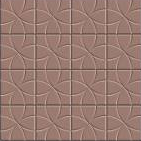
\includegraphics[width=\scaleFactor cm, height=\scaleFactor cm] {%
				\PATH one_shots/stylesheets/images/textures/red_concrete_path.png%
			}%
		};%
		\foreach \x in {1,...,8}{%
			\node at (\dimexpr{0.5\paperwidth - \x cm}, \y) {%
				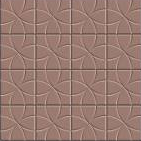
\includegraphics[width=\scaleFactor cm, height=\scaleFactor cm] {%
					\PATH one_shots/stylesheets/images/textures/red_concrete_path.png%
				}%
			};%
			\node at (\dimexpr{0.5\paperwidth + \x cm}, \y) {%
				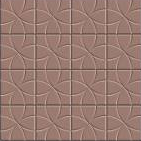
\includegraphics[width=\scaleFactor cm, height=\scaleFactor cm] {%
					\PATH one_shots/stylesheets/images/textures/red_concrete_path.png%
				}%
			};%
		}%
	}%
\end{scope}
% Grass
\begin{scope}[scale=0.25, xshift=2\paperwidth, yshift=\verticalOffset]
	\path[clip] (34,5)
		-- ++(-7,0) -- ++(0,1) -- ++(-1,0) -- ++(0,6) -- ++(6,0) -- ++(0,5) -- ++(-4,0) -- ++(-2,5) -- ++(-5,2) -- ++(0,3.75) -- ++(-29,0) -- ++(0,1.25) -- ++(-23,0) -- ++(0,-42) -- ++(-1,0) -- ++(0,-5) -- ++(4,0) -- ++(2,-5) -- ++(5,-2) -- ++(0,-4) -- ++(5,0) -- ++(0,7) -- ++(4,0) -- ++(0,-7) -- ++(24,0) -- ++(0,7) -- ++(4,0) -- ++(0,-7) -- ++(5,0) -- ++(0,4) -- ++(2,5) -- ++(5,2) -- ++(4,0) -- ++(0,5) -- ++(-6,0) -- ++(0,6) -- ++(1,0) -- ++(0,1) -- ++(7,0)
		-- ++(0,-27) -- ++(-68,0) -- ++(0,64) -- ++(68,0) -- cycle;
	\foreach \x in {0,...,16}{%
		\foreach \y in {0,...,16}{%
			\node at (-32 + 4*\x, 30 - 4*\y) {%
				\includegraphics[width=\scaleFactor cm, height=\scaleFactor cm] {%
					\ASSETPATH Textures/Natural_Textures/Grass/Short_Grass_C_01%
				}%
			};%
		}%
	}%
\end{scope}
% #-#-#-#-#-#-#-#-#-#-#-#-#-#-#-#-#-#-#-#-#-#-#-#-#-#-#-#-#-#-#-#-#-#-#-#-#-#-#-#-#-#-#-#-#-#-#-#-#-#-#-#-#-#-#-#-# %
% -------------------------------------------------- % Stairs % --------------------------------------------------- %
% #-#-#-#-#-#-#-#-#-#-#-#-#-#-#-#-#-#-#-#-#-#-#-#-#-#-#-#-#-#-#-#-#-#-#-#-#-#-#-#-#-#-#-#-#-#-#-#-#-#-#-#-#-#-#-#-# %
% Middle
\begin{scope}[scale=0.25, xshift=2\paperwidth, yshift=\verticalOffset]
	\pgfmathsetmacro{\scaledWidth}{0.75*\scaleFactor}
	\pgfmathsetmacro{\scaledHeight}{0.4*\scaleFactor}
	\pgfmathsetmacro{\scaledDimension}{0.5*\scaleFactor}
	%% South East
	% Stair
	\begin{scope}
		\path[clip] (11,-12)
			-- ++(2,2) -- ++(-1.5,1.5) -- ++(-2,-2) -- cycle;
		\node[inner sep=0pt,outer sep=0pt,clip,rotate=-135] at (11.15,-10.15) {%
			\includegraphics[width=\scaledWidth cm, height=\scaledHeight cm] {%
				\ASSETPATH/Structures/Stairs_and_Ladders/Stairs_Stone/Stairs_Stone_Earthy_C_1x1.png%
			}%
		};%
	\end{scope}
	% Shadow
	\begin{scope}
		\path[clip] (13,-6)
			-- ++(0,-4) -- ++(1,0) -- ++(0,4) -- cycle;
		\path[drop shadow] (13,-6)
			-- ++(0,-4) -- ++(-1,0) -- ++(0,4) -- cycle;
	\end{scope}
	\begin{scope}
		\path[clip] (7,-12)
			-- ++(4,0) -- ++(0,-1) -- ++(-4,0) -- cycle;
		\path[drop shadow] (7,-12)
			-- ++(4,0) -- ++(0,1) -- ++(-4,0) -- cycle;
	\end{scope}
	% Walls
	\node[inner sep=0pt,outer sep=0pt,clip,rotate=135] at (10.25,-11.25) {%
		\includegraphics[height=\scaledDimension cm,keepaspectratio] {%
			\ASSETPATH/Structures/Walls_and_Curbs/Curb_Stone_A/Curb_Stone_Redrock_A_Straight_C_1x1%
		}%
	};%
	\node[inner sep=0pt,outer sep=0pt,clip] at (10,-12) {%
		\includegraphics[height=\scaledDimension cm,keepaspectratio] {%
			\ASSETPATH/Structures/Walls_and_Curbs/Curb_Stone_A/Curb_Stone_Redrock_A_Straight_C_1x1%
		}%
	};
	\node[inner sep=0pt,outer sep=0pt,clip,rotate=180] at (8,-12) {%
		\includegraphics[height=\scaledDimension cm,keepaspectratio] {%
			\ASSETPATH/Structures/Walls_and_Curbs/Curb_Stone_A/Curb_Stone_Redrock_A_Straight_C_1x1%
		}%
	};%
	\node[inner sep=0pt,outer sep=0pt,clip,rotate=135] at (12.25,-9.25) {%
		\includegraphics[height=\scaledDimension cm,keepaspectratio] {%
			\ASSETPATH/Structures/Walls_and_Curbs/Curb_Stone_A/Curb_Stone_Redrock_A_Straight_C_1x1%
		}%
	};%
	\node[inner sep=0pt,outer sep=0pt,clip,rotate=-90] at (13,-9) {%
		\includegraphics[height=\scaledDimension cm,keepaspectratio] {%
			\ASSETPATH/Structures/Walls_and_Curbs/Curb_Stone_A/Curb_Stone_Redrock_A_Straight_C_1x1%
		}%
	};%
	\node[inner sep=0pt,outer sep=0pt,clip,rotate=90] at (13,-7) {%
		\includegraphics[height=\scaledDimension cm,keepaspectratio] {%
			\ASSETPATH/Structures/Walls_and_Curbs/Curb_Stone_A/Curb_Stone_Redrock_A_Straight_C_1x1%
		}%
	};%
	%% South West
	% Stair
	\begin{scope}
		\path[clip] (-11,-12)
			-- ++(-2,2) -- ++(1.5,1.5) -- ++(2,-2) -- cycle;
		\node[inner sep=0pt,outer sep=0pt,clip,rotate=135] at (-11.15,-10.15) {%
			\includegraphics[width=\scaledWidth cm, height=\scaledHeight cm] {%
				\ASSETPATH/Structures/Stairs_and_Ladders/Stairs_Stone/Stairs_Stone_Earthy_C_1x1.png%
			}%
		};%
	\end{scope}
	% Shadow
	\begin{scope}
		\path[clip] (-7,-12)
			-- ++(-4,0) -- ++(0,-1) -- ++(4,0) -- cycle;
		\path[drop shadow] (-7,-12)
			-- ++(-4,0) -- ++(0,1) -- ++(4,0) -- cycle;
	\end{scope}
	\begin{scope}
		\path[clip] (-9.5,-10.5)
			-- ++(-1.5,-1.5) -- ++(1,-1) -- ++(1.5,1.5) -- cycle;
		\path[drop shadow] (-9.5,-10.5)
			-- ++(-1.5,-1.5) -- ++(-1,1) -- ++(1.5,1.5) -- cycle;
	\end{scope}
	\begin{scope}
		\path[clip] (-13,-6)
			-- ++(0,-4) -- ++(1.5,1.5) -- cycle;
		\path[drop shadow] (-13,-6)
			-- ++(0,-4) -- ++(-1,0) -- ++(0,4) -- cycle;
	\end{scope}
	\begin{scope}
		\path[clip] (-11.5,-8.5)
			-- ++(-1.5,-1.5) -- ++(1,-1) -- ++(1.5,1.5) -- cycle;
		\path[drop shadow] (-11.5,-8.5)
			-- ++(-1.5,-1.5) -- ++(-1,1) -- ++(1.5,1.5) -- cycle;
	\end{scope}
	% Walls
	\node[inner sep=0pt,outer sep=0pt,clip,rotate=45] at (-10.25,-11.25) {%
		\includegraphics[height=\scaledDimension cm,keepaspectratio] {%
			\ASSETPATH/Structures/Walls_and_Curbs/Curb_Stone_A/Curb_Stone_Redrock_A_Straight_C_1x1%
		}%
	};%
	\node[inner sep=0pt,outer sep=0pt,clip,rotate=180] at (-10,-12) {%
		\includegraphics[height=\scaledDimension cm,keepaspectratio] {%
			\ASSETPATH/Structures/Walls_and_Curbs/Curb_Stone_A/Curb_Stone_Redrock_A_Straight_C_1x1%
		}%
	};%
	\node[inner sep=0pt,outer sep=0pt,clip] at (-8,-12) {%
		\includegraphics[height=\scaledDimension cm,keepaspectratio] {%
			\ASSETPATH/Structures/Walls_and_Curbs/Curb_Stone_A/Curb_Stone_Redrock_A_Straight_C_1x1%
		}%
	};%
	\node[inner sep=0pt,outer sep=0pt,clip,rotate=45] at (-12.25,-9.25) {%
		\includegraphics[height=\scaledDimension cm,keepaspectratio] {%
			\ASSETPATH/Structures/Walls_and_Curbs/Curb_Stone_A/Curb_Stone_Redrock_A_Straight_C_1x1%
		}%
	};%
	\node[inner sep=0pt,outer sep=0pt,clip,rotate=-90] at (-13,-9) {%
		\includegraphics[height=\scaledDimension cm,keepaspectratio] {%
			\ASSETPATH/Structures/Walls_and_Curbs/Curb_Stone_A/Curb_Stone_Redrock_A_Straight_C_1x1%
		}%
	};%
	\node[inner sep=0pt,outer sep=0pt,clip,rotate=90] at (-13,-7) {%
		\includegraphics[height=\scaledDimension cm,keepaspectratio] {%
			\ASSETPATH/Structures/Walls_and_Curbs/Curb_Stone_A/Curb_Stone_Redrock_A_Straight_C_1x1%
		}%
	};%
	%% North West
	% Stair
	\begin{scope}
		\path[clip] (-11,11)
			-- ++(-2,-2) -- ++(1.5,-1.5) -- ++(2,2) -- cycle;
		\node[inner sep=0pt,outer sep=0pt,clip,rotate=45] at (-11.15,9.15) {%
			\includegraphics[width=\scaledWidth cm, height=\scaledHeight cm] {%
				\ASSETPATH/Structures/Stairs_and_Ladders/Stairs_Stone/Stairs_Stone_Earthy_C_1x1.png%
			}%
		};%
	\end{scope}
	% Shadow
	\begin{scope}
		\path[clip] (-13,5)
			-- ++(0,4) -- ++(1.5,-1.5) -- cycle;
		\path[drop shadow] (-13,5)
			-- ++(0,4) -- ++(-1,0) -- ++(0,-4) -- cycle;
	\end{scope}
	\begin{scope}
		\path[clip] (-7,11)
			-- ++(-4,0) -- ++(1.5,-1.5) -- cycle;
		\path[drop shadow] (-7,11)
			-- ++(-4,0) -- ++(0,1) -- ++(4,0) -- cycle;
	\end{scope}
	% Walls
	\node[inner sep=0pt,outer sep=0pt,clip,rotate=-45] at (-10.25,10.25) {%
		\includegraphics[height=\scaledDimension cm,keepaspectratio] {%
			\ASSETPATH/Structures/Walls_and_Curbs/Curb_Stone_A/Curb_Stone_Redrock_A_Straight_C_1x1%
		}%
	};%
	\node[inner sep=0pt,outer sep=0pt,clip,rotate=180] at (-10,11) {%
		\includegraphics[height=\scaledDimension cm,keepaspectratio] {%
			\ASSETPATH/Structures/Walls_and_Curbs/Curb_Stone_A/Curb_Stone_Redrock_A_Straight_C_1x1%
		}%
	};%
	\node[inner sep=0pt,outer sep=0pt,clip] at (-8,11) {%
		\includegraphics[height=\scaledDimension cm,keepaspectratio] {%
			\ASSETPATH/Structures/Walls_and_Curbs/Curb_Stone_A/Curb_Stone_Redrock_A_Straight_C_1x1%
		}%
	};%
	\node[inner sep=0pt,outer sep=0pt,clip,rotate=-45] at (-12.25,8.25) {%
		\includegraphics[height=\scaledDimension cm,keepaspectratio] {%
			\ASSETPATH/Structures/Walls_and_Curbs/Curb_Stone_A/Curb_Stone_Redrock_A_Straight_C_1x1%
		}%
	};%
	\node[inner sep=0pt,outer sep=0pt,clip,rotate=90] at (-13,8) {%
		\includegraphics[height=\scaledDimension cm,keepaspectratio] {%
			\ASSETPATH/Structures/Walls_and_Curbs/Curb_Stone_A/Curb_Stone_Redrock_A_Straight_C_1x1%
		}%
	};%
	\node[inner sep=0pt,outer sep=0pt,clip,rotate=-90] at (-13,6) {%
		\includegraphics[height=\scaledDimension cm,keepaspectratio] {%
			\ASSETPATH/Structures/Walls_and_Curbs/Curb_Stone_A/Curb_Stone_Redrock_A_Straight_C_1x1%
		}%
	};%
	%% North East
	% Stair
	\begin{scope}
		\path[clip] (11,11)
			-- ++(2,-2) -- ++(-1.5,-1.5) -- ++(-2,2) -- cycle;
		\node[inner sep=0pt,outer sep=0pt,clip,rotate=-45] at (11.15,9.15) {%
			\includegraphics[width=\scaledWidth cm, height=\scaledHeight cm] {%
				\ASSETPATH/Structures/Stairs_and_Ladders/Stairs_Stone/Stairs_Stone_Earthy_C_1x1.png%
			}%
		};%
	\end{scope}
	% Shadow
	\begin{scope}
		\path[clip] (7,11)
			-- ++(4,0) -- ++(-1.5,-1.5) -- cycle;
		\path[drop shadow] (7,11)
			-- ++(4,0) -- ++(0,1) -- ++(-4,0) -- cycle;
	\end{scope}
	\begin{scope}
		\path[clip] (11,11)
			-- ++(-1.5,-1.5) -- ++(1,-1) -- ++(1.5,1.5) -- cycle;
		\path[drop shadow] (11,11)
			-- ++(-1.5,-1.5) -- ++(-1,1) -- ++(1.5,1.5) -- cycle;
	\end{scope}
	\begin{scope}
		\path[clip] (13,5)
			-- ++(0,4) -- ++(1.5,-1.5) -- cycle;
		\path[drop shadow] (13,5)
			-- ++(0,4) -- ++(-1,0) -- ++(0,-4) -- cycle;
	\end{scope}
	\begin{scope}
		\path[clip] (13,9)
			-- ++(-1.5,-1.5) -- ++(1,-1) -- ++(1.5,1.5) -- cycle;
		\path[drop shadow] (13,9)
			-- ++(-1.5,-1.5) -- ++(-1,1) -- ++(1.5,1.5) -- cycle;
	\end{scope}
	% Walls
	\node[inner sep=0pt,outer sep=0pt,clip,rotate=-135] at (10.25,10.25) {%
		\includegraphics[height=\scaledDimension cm,keepaspectratio] {%
			\ASSETPATH/Structures/Walls_and_Curbs/Curb_Stone_A/Curb_Stone_Redrock_A_Straight_C_1x1%
		}%
	};%
	\node[inner sep=0pt,outer sep=0pt,clip] at (10,11) {%
		\includegraphics[height=\scaledDimension cm,keepaspectratio] {%
			\ASSETPATH/Structures/Walls_and_Curbs/Curb_Stone_A/Curb_Stone_Redrock_A_Straight_C_1x1%
		}%
	};%
	\node[inner sep=0pt,outer sep=0pt,clip,rotate=180] at (8,11) {%
		\includegraphics[height=\scaledDimension cm,keepaspectratio] {%
			\ASSETPATH/Structures/Walls_and_Curbs/Curb_Stone_A/Curb_Stone_Redrock_A_Straight_C_1x1%
		}%
	};%
	\node[inner sep=0pt,outer sep=0pt,clip,rotate=-135] at (12.25,8.25) {%
		\includegraphics[height=\scaledDimension cm,keepaspectratio] {%
			\ASSETPATH/Structures/Walls_and_Curbs/Curb_Stone_A/Curb_Stone_Redrock_A_Straight_C_1x1%
		}%
	};%
	\node[inner sep=0pt,outer sep=0pt,clip,rotate=90] at (13,8) {%
		\includegraphics[height=\scaledDimension cm,keepaspectratio] {%
			\ASSETPATH/Structures/Walls_and_Curbs/Curb_Stone_A/Curb_Stone_Redrock_A_Straight_C_1x1%
		}%
	};%
	\node[inner sep=0pt,outer sep=0pt,clip,rotate=-90] at (13,6) {%
		\includegraphics[height=\scaledDimension cm,keepaspectratio] {%
			\ASSETPATH/Structures/Walls_and_Curbs/Curb_Stone_A/Curb_Stone_Redrock_A_Straight_C_1x1%
		}%
	};%
\end{scope}
% #-#-#-#-#-#-#-#-#-#-#-#-#-#-#-#-#-#-#-#-#-#-#-#-#-#-#-#-#-#-#-#-#-#-#-#-#-#-#-#-#-#-#-#-#-#-#-#-#-#-#-#-#-#-#-#-# %
% ---------------------------------------------- % Penguin Habitat % ---------------------------------------------- %
% #-#-#-#-#-#-#-#-#-#-#-#-#-#-#-#-#-#-#-#-#-#-#-#-#-#-#-#-#-#-#-#-#-#-#-#-#-#-#-#-#-#-#-#-#-#-#-#-#-#-#-#-#-#-#-#-# %
\begin{scope}[scale=0.25, xshift=2\paperwidth, yshift=\verticalOffset]
	\path[clip] (0,2)
		-- ++(3,0) -- ++(1,-1) -- ++(0,-3) -- ++(-1,-1) -- ++(-6,0) -- ++(-1,1) -- ++(0,3) -- ++(1,1) -- cycle;
	\node[inner sep=0pt,outer sep=0pt,clip] {%
		\pgfmathsetmacro{\scaledWidth}{2*\scaleFactor}%
		\pgfmathsetmacro{\scaledHeight}{1.5*\scaleFactor}%
		\includegraphics[width=\scaledWidth cm, height=\scaledHeight cm] {%
			\ASSETPATH/Textures/Natural_Textures/Water/Water_Opaque_A_03%
		}%
	};%
\end{scope}
\begin{scope}[scale=0.25, xshift=2\paperwidth, yshift=\verticalOffset]
	\path[clip] (0,2.5) -- ++(3.2,0) -- ++(1.3,-1.3) -- ++(0,-3.4) -- ++(-1.3,-1.3) -- ++(-6.4,0) -- ++(-1.3,1.3) -- ++(0,3.4) -- ++(1.3,1.3) -- cycle;
	\path[clip,drop shadow] (-3,2.5)
		-- ++(3,0) -- ++(0,-0.5) -- ++(-3,0) -- ++(-1,-1) -- ++(0,-3) -- ++(1,-1) -- ++(6,0) -- ++(1,1) -- ++(0,3) -- ++(-1,1) -- ++(-3,0) -- ++(0,0.5)
		++(3.2,0) -- ++(1.3,-1.3) -- ++(0,-3.4) -- ++(-1.3,-1.3) -- ++(-6.4,0) -- ++(-1.3,1.3) -- ++(0,3.4) -- ++(1.3,1.3) -- cycle;
	\node[inner sep=0pt,outer sep=0pt, clip] {%
		\pgfmathsetmacro{\scaledWidth}{2.5*\scaleFactor}%
		\pgfmathsetmacro{\scaledHeight}{2*\scaleFactor}%
		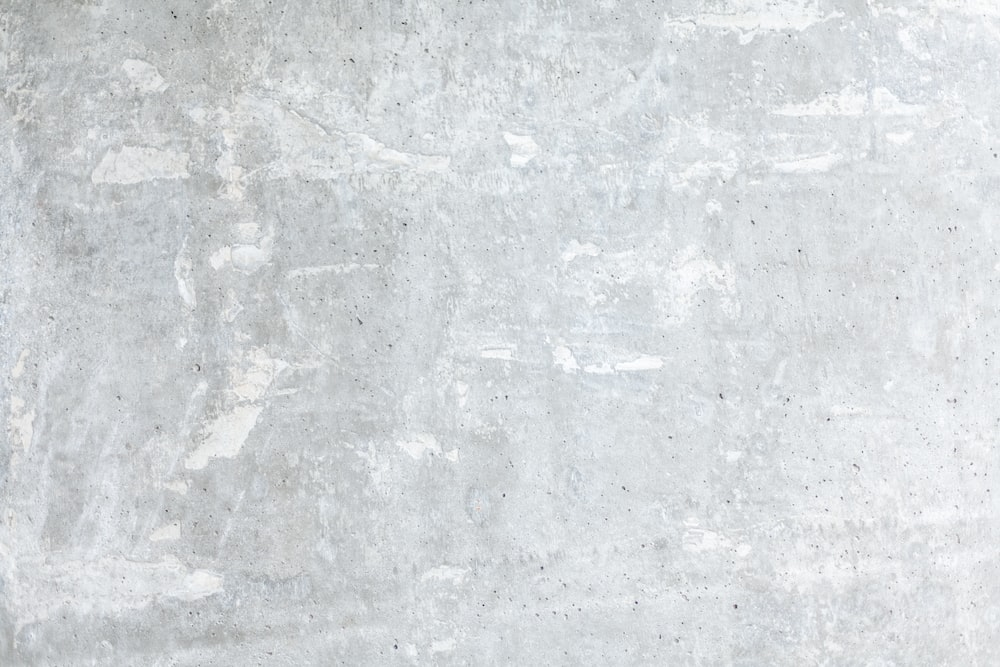
\includegraphics[width=\scaledWidth cm, height=\scaledHeight cm] {%
			\PATH one_shots/stylesheets/images/textures/concrete.jpeg%
		}%
	};%
	\path[draw, black, thick] (0,2.25) -- ++(3.1,0) -- ++(1.15,-1.15) -- ++(0,-3.2) -- ++(-1.15,-1.15) -- ++(-6.2,0) -- ++(-1.15,1.15) -- ++(0,3.2) -- ++(1.15,1.15) -- cycle;
\end{scope}
% Assets
\begin{scope}[scale=0.25, xshift=2\paperwidth, yshift=\verticalOffset]
	% Foam
	\node[inner sep=0pt,outer sep=0pt,rotate=180] at (0,-2.1) {%
		\pgfmathsetmacro{\scaledWidth}{1.5*\scaleFactor}%
		\pgfmathsetmacro{\scaledHeight}{1.2*\scaleFactor}%
		\includegraphics[width=\scaledWidth cm, height=\scaledHeight cm] {%
			\ASSETPATH/Terrain/Water/Foam/Water_Foam_Flow_A6_1x1%
		}%
	};%
	\node[inner sep=0pt,outer sep=0pt,rotate=90] at (1.5,-0.5) {%
		\pgfmathsetmacro{\scaledWidth}{1*\scaleFactor}%
		\pgfmathsetmacro{\scaledHeight}{1*\scaleFactor}%
		\includegraphics[width=\scaledWidth cm, height=\scaledHeight cm] {%
			\ASSETPATH/Terrain/Water/Foam/Water_Foam_Flow_C8_1x1%
		}%
	};%
	\node[inner sep=0pt,outer sep=0pt,rotate=40] at (-1.6,0.85) {%
		\pgfmathsetmacro{\scaledWidth}{1*\scaleFactor}%
		\pgfmathsetmacro{\scaledHeight}{0.7*\scaleFactor}%
		\includegraphics[width=\scaledWidth cm, height=\scaledHeight cm] {%
			\ASSETPATH/Terrain/Water/Foam/Water_Foam_Flow_C6_2x1%
		}%
	};%
	\node[inner sep=0pt,outer sep=0pt,rotate=100] at (-2.7,-0.85) {%
		\pgfmathsetmacro{\scaledWidth}{1.2*\scaleFactor}%
		\pgfmathsetmacro{\scaledHeight}{0.8*\scaleFactor}%
		\includegraphics[width=\scaledWidth cm, height=\scaledHeight cm] {%
			\ASSETPATH/Terrain/Water/Foam/Water_Foam_Flow_A2_2x1%
		}%
	};%
	\node[inner sep=0pt,outer sep=0pt,rotate=135] at (2.5,1) {%
		\pgfmathsetmacro{\scaledWidth}{0.9*\scaleFactor}%
		\pgfmathsetmacro{\scaledHeight}{0.6*\scaleFactor}%
		\includegraphics[width=\scaledWidth cm, height=\scaledHeight cm] {%
			\ASSETPATH/Terrain/Water/Foam/Water_Foam_Medium_B1_2x1%
		}%
	};
	% Rocks%
	\node[inner sep=0pt,outer sep=0pt,rotate=170] at (-1.5,-1) {%
		\pgfmathsetmacro{\scaledWidth}{0.6*\scaleFactor}%
		\pgfmathsetmacro{\scaledHeight}{0.4*\scaleFactor}%
		\includegraphics[width=\scaledWidth cm, height=\scaledHeight cm, keepaspectratio] {%
			\ASSETPATH/Natural_Decor/Rocks/Boulders/Boulder_Stone_Slate_C9_3x2%
		}%
	};%
	\node[inner sep=0pt,outer sep=0pt,rotate=45] at (1.3,-1.3) {%
		\pgfmathsetmacro{\scaledWidth}{0.6*\scaleFactor}%
		\pgfmathsetmacro{\scaledHeight}{0.4*\scaleFactor}%
		\includegraphics[width=\scaledWidth cm, height=\scaledHeight cm, keepaspectratio] {%
			\ASSETPATH/Natural_Decor/Rocks/Boulders/Boulder_Stone_Slate_C8_3x2%
		}%
	};%
	\node[inner sep=0pt,outer sep=0pt] at (0,-1.8) {%
		\pgfmathsetmacro{\scaledWidth}{0.7*\scaleFactor}%
		\pgfmathsetmacro{\scaledHeight}{0.7*\scaleFactor}%
		\includegraphics[width=\scaledWidth cm, height=\scaledHeight cm, keepaspectratio] {%
			\ASSETPATH/Natural_Decor/Rocks/Boulders/Boulder_Stone_Slate_C18_2x2%
		}%
	};%
	\node[inner sep=0pt,outer sep=0pt,rotate=-135] at (0.9,0.4) {%
		\pgfmathsetmacro{\scaledWidth}{0.4*\scaleFactor}%
		\pgfmathsetmacro{\scaledHeight}{0.6*\scaleFactor}%
		\includegraphics[width=\scaledWidth cm, height=\scaledHeight cm, keepaspectratio] {%
			\ASSETPATH/Natural_Decor/Rocks/Boulders/Boulder_Stone_Slate_B13_2x3%
		}%
	};%
	\node[inner sep=0pt,outer sep=0pt] at (0,-0.5) {%
		\pgfmathsetmacro{\scaledWidth}{0.8*\scaleFactor}%
		\pgfmathsetmacro{\scaledHeight}{0.8*\scaleFactor}%
		\includegraphics[width=\scaledWidth cm, height=\scaledHeight cm, keepaspectratio] {%
			\ASSETPATH/Natural_Decor/Rocks/Boulders/Boulder_Stone_Slate_D9_2x2%
		}%
	};%
\end{scope}
% #-#-#-#-#-#-#-#-#-#-#-#-#-#-#-#-#-#-#-#-#-#-#-#-#-#-#-#-#-#-#-#-#-#-#-#-#-#-#-#-#-#-#-#-#-#-#-#-#-#-#-#-#-#-#-#-# %
% ------------------------------------------- % Lemur Habitat  (West) % ------------------------------------------- %
% #-#-#-#-#-#-#-#-#-#-#-#-#-#-#-#-#-#-#-#-#-#-#-#-#-#-#-#-#-#-#-#-#-#-#-#-#-#-#-#-#-#-#-#-#-#-#-#-#-#-#-#-#-#-#-#-# %
\begin{scope}[scale=0.25, xshift=2\paperwidth, yshift=\verticalOffset]
	\path[clip] (-8,0)
		-- ++(0,-3) -- ++(-4,-4) -- ++(-1,1) -- ++(0,11) -- ++(1,1) -- ++(4,-4) -- cycle;
	\foreach \y in {0,...,3}{
		\node[inner sep=0pt,outer sep=0pt,clip] at (-11.5,4 - 4*\y) {%
			\pgfmathsetmacro{\scaledWidth}{1*\scaleFactor}%
			\pgfmathsetmacro{\scaledHeight}{1*\scaleFactor}%
			\includegraphics[width=\scaledWidth cm, height=\scaledHeight cm] {%
				\ASSETPATH/Textures/Natural_Textures/Grass/Grass_C_01%
			}%
		};%
	}	
	\path[clip, draw] (-8,0)
		-- ++(0,2) -- ++(-2,2) arc[start angle=160, end angle=195, radius=4] arc[start angle=15, end angle=-10, radius=9] arc[start angle=170, end angle=205, radius=5] -- (-8,-3) -- cycle;
	\foreach \y in {0,...,2}{
		\node[inner sep=0pt,outer sep=0pt,clip] at (-9,2.5 - 3*\y) {%
			\pgfmathsetmacro{\scaledWidth}{0.75*\scaleFactor}%
			\pgfmathsetmacro{\scaledHeight}{0.75*\scaleFactor}%
			\includegraphics[width=\scaledWidth cm, height=\scaledHeight cm] {%
				\ASSETPATH/Textures/Natural_Textures/Misc/Terrain_A_09%
			}%
		};%
	}
	\path[clip, draw] (-8,0)
		-- ++(0,2) -- ++(-1.5,1.5) arc[start angle=165, end angle=215, radius=3] arc[start angle=35, end angle=-25, radius=2.5] arc[start angle=155, end angle=205, radius=3] -- (-8,-3) -- cycle;
	\foreach \y in {0,...,5}{
		\node[inner sep=0pt,outer sep=0pt,clip] at (-8.7,2.5 - 2*\y) {%
			\pgfmathsetmacro{\scaledWidth}{0.5*\scaleFactor}%
			\pgfmathsetmacro{\scaledHeight}{0.5*\scaleFactor}%
			\includegraphics[width=\scaledWidth cm, height=\scaledHeight cm] {%
				\ASSETPATH/Textures/Natural_Textures/Water/Water_Opaque_A_03%
			}%
		};%
	}
	
\end{scope}
% Volcano Base
\begin{scope}[scale=0.25, xshift=2\paperwidth, yshift=\verticalOffset]
	\node[inner sep=0pt,outer sep=0pt,clip] at (-13,-5) {%
		\pgfmathsetmacro{\scaledWidth}{1*\scaleFactor}%
		\pgfmathsetmacro{\scaledHeight}{1*\scaleFactor}%
		\includegraphics[width=\scaledWidth cm, height=\scaledHeight cm] {%
			\ASSETPATH/Natural_Decor/Rocks/Boulders/Boulder_Stone_Volcanic_B28_2x2%
		}%
	};%
\end{scope}
% Outer Wall
\begin{scope}[scale=0.25, xshift=2\paperwidth, yshift=\verticalOffset]
	\path[clip, drop shadow] (-7.5,0)
		-- ++(-0.5,0) -- ++(0,-3) -- ++(-4,-4) -- ++(-1,1) -- ++(0,11) -- ++(1,1) -- ++(4,-4) -- ++(0,-2) -- ++(0.5,0)
		-- ++(0,2.2) -- ++(-4.3,4.3) -- ++(-0.41,0) -- ++(-1.3,-1.3) -- ++(0,-11.41) -- ++(1.3,-1.3) -- ++(0.41,0) -- ++(4.3,4.3) -- cycle;
\end{scope}
\begin{scope}[scale=0.25, xshift=2\paperwidth, yshift=\verticalOffset]
	% Straight Walls
	\node[inner sep=0pt,outer sep=0pt,clip,rotate=90] at (-13.25,2.2) {%
		\pgfmathsetmacro{\scaledHeight}{0.6*\scaleFactor}%
		\includegraphics[height=\scaledHeight cm, keepaspectratio] {%
			\ASSETPATH/Structures/Railings_and_Fences/Fence_Stone_A/Fence_Stone_Earthy_A_Straight_B_2x1%
		}%
	};%
	\node[inner sep=0pt,outer sep=0pt,clip,rotate=90] at (-13.25,-2.85) {%
		\pgfmathsetmacro{\scaledHeight}{0.6*\scaleFactor}%
		\includegraphics[height=\scaledHeight cm, keepaspectratio] {%
			\ASSETPATH/Structures/Railings_and_Fences/Fence_Stone_A/Fence_Stone_Earthy_A_Straight_B_2x1%
		}%
	};%
	\node[inner sep=0pt,outer sep=0pt,clip,rotate=90] at (-13.25,0) {%
		\pgfmathsetmacro{\scaledHeight}{0.6*\scaleFactor}%
		\includegraphics[height=\scaledHeight cm, keepaspectratio] {%
			\ASSETPATH/Structures/Railings_and_Fences/Fence_Stone_A/Fence_Stone_Earthy_A_Straight_C_1x1%
		}%
	};%
	\node[inner sep=0pt,outer sep=0pt,clip,rotate=90] at (-7.8,-0.5) {%
		\pgfmathsetmacro{\scaledHeight}{0.6*\scaleFactor}%
		\includegraphics[height=\scaledHeight cm, keepaspectratio] {%
			\ASSETPATH/Structures/Railings_and_Fences/Fence_Stone_A/Fence_Stone_Earthy_A_Straight_B_2x1%
		}%
	};%
	\node[inner sep=0pt,outer sep=0pt,clip,rotate=-45] at (-9.95,4.25) {%
		\pgfmathsetmacro{\scaledHeight}{0.6*\scaleFactor}%
		\includegraphics[height=\scaledHeight cm, keepaspectratio] {%
			\ASSETPATH/Structures/Railings_and_Fences/Fence_Stone_A/Fence_Stone_Earthy_A_Straight_B_2x1%
		}%
	};%
	\node[inner sep=0pt,outer sep=0pt,clip,rotate=45] at (-9.65,-5) {%
		\pgfmathsetmacro{\scaledHeight}{0.6*\scaleFactor}%
		\includegraphics[height=\scaledHeight cm, keepaspectratio] {%
			\ASSETPATH/Structures/Railings_and_Fences/Fence_Stone_A/Fence_Stone_Earthy_A_Straight_B_2x1%
		}%
	};%
	\node[inner sep=0pt,outer sep=0pt,clip,rotate=-45] at (-12,6.325) {%
		\pgfmathsetmacro{\scaledHeight}{0.6*\scaleFactor}%
		\includegraphics[height=\scaledHeight cm, keepaspectratio] {%
			\ASSETPATH/Structures/Railings_and_Fences/Fence_Stone_A/Fence_Stone_Earthy_A_Corner_A_1x1%
		}%
	};%
	\node[inner sep=0pt,outer sep=0pt,clip,rotate=135] at (-12,-7.325) {%
		\pgfmathsetmacro{\scaledHeight}{0.6*\scaleFactor}%
		\includegraphics[height=\scaledHeight cm, keepaspectratio] {%
			\ASSETPATH/Structures/Railings_and_Fences/Fence_Stone_A/Fence_Stone_Earthy_A_Corner_A_1x1%
		}%
	};%
	% Connectors%
	\node[inner sep=0pt,outer sep=0pt,clip,rotate=45] at (-13.25,5.05) {%
		\pgfmathsetmacro{\scaledHeight}{0.6*\scaleFactor}%
		\includegraphics[height=\scaledHeight cm, keepaspectratio] {%
			\ASSETPATH/Structures/Railings_and_Fences/Fence_Stone_A/Fence_Stone_Earthy_A_Connector_DIAG_A_1x1%
		}%
	};%
	\node[inner sep=0pt,outer sep=0pt,clip,rotate=90] at (-13.225,-6.05) {%
		\pgfmathsetmacro{\scaledHeight}{0.6*\scaleFactor}%
		\includegraphics[height=\scaledHeight cm, keepaspectratio] {%
			\ASSETPATH/Structures/Railings_and_Fences/Fence_Stone_A/Fence_Stone_Earthy_A_Connector_DIAG_A_1x1%
		}%
	};%
	\node[inner sep=0pt,outer sep=0pt,clip,rotate=-90] at (-7.75,2.1) {%
		\pgfmathsetmacro{\scaledHeight}{0.6*\scaleFactor}%
		\includegraphics[height=\scaledHeight cm, keepaspectratio] {%
			\ASSETPATH/Structures/Railings_and_Fences/Fence_Stone_A/Fence_Stone_Earthy_A_Connector_DIAG_A_1x1%
		}%
	};%
	\node[inner sep=0pt,outer sep=0pt,clip,rotate=-135] at (-7.8,-3.05) {%
		\pgfmathsetmacro{\scaledHeight}{0.6*\scaleFactor}%
		\includegraphics[height=\scaledHeight cm, keepaspectratio] {%
			\ASSETPATH/Structures/Railings_and_Fences/Fence_Stone_A/Fence_Stone_Earthy_A_Connector_DIAG_A_1x1%
		}%
	};%
\end{scope}
% Volcano Top
\begin{scope}[scale=0.25, xshift=2\paperwidth, yshift=\verticalOffset]
	\node[inner sep=0pt,outer sep=0pt,clip] at (-13,-5) {%
		\pgfmathsetmacro{\scaledWidth}{0.75*\scaleFactor}%
		\pgfmathsetmacro{\scaledHeight}{0.75*\scaleFactor}%
		\includegraphics[width=\scaledWidth cm, height=\scaledHeight cm] {%
			\ASSETPATH/Natural_Decor/Rocks/Boulders/Boulder_Stone_Volcanic_B17_2x2%
		}%
	};%
	\node[inner sep=0pt,outer sep=0pt,clip] at (-13,-5) {%
		\pgfmathsetmacro{\scaledWidth}{0.45*\scaleFactor}%
		\pgfmathsetmacro{\scaledHeight}{0.45*\scaleFactor}%
		\includegraphics[width=\scaledWidth cm, height=\scaledHeight cm] {%
			\ASSETPATH/Overlays_and_Effects/Fire/Fire_red_A36_1x1%
		}%
	};%
\end{scope}
% Assets
\begin{scope}[scale=0.25, xshift=2\paperwidth, yshift=\verticalOffset]
	\path[clip] (-8,0)
		-- ++(0,-3) -- ++(-4,-4) -- ++(-1,1) -- ++(0,11) -- ++(1,1) -- ++(4,-4) -- cycle;
	\path[drop shadow] (-10.6,-0.5)
		-- ++(1,1) -- ++(0,-2) -- ++(-2,0) -- ++(0,2) -- ++(2,0) -- cycle;
	\node[inner sep=0pt,outer sep=0pt,clip] at (-10.6,-0.5) {%
		\pgfmathsetmacro{\scaledWidth}{0.75*\scaleFactor}%
		\pgfmathsetmacro{\scaledHeight}{0.75*\scaleFactor}%
		\includegraphics[width=\scaledWidth cm, height=\scaledHeight cm] {%
			\ASSETPATH/Structures/Pillars/Pillar_Stone_Slate_D1_1x1%
		}%
	};%
	\node[inner sep=0pt,outer sep=0pt,clip] at (-10.7,-0.85) {%
		\pgfmathsetmacro{\scaledWidth}{0.3*\scaleFactor}%
		\pgfmathsetmacro{\scaledHeight}{0.3*\scaleFactor}%
		\includegraphics[width=\scaledWidth cm, height=\scaledHeight cm] {%
			\ASSETPATH/Furniture/Seating/Ottomans/Ottoman_Fabric_Yellow_Wood_Ashen_A2_1x1%
		}%
	};%
	\path[drop shadow] (-11.25,-1)
		-- ++(0.35,0) arc[start angle=0, end angle=360, radius=0.35] -- cycle;
	\node[inner sep=0pt,outer sep=0pt,clip] at (-11.25,-1) {%
		\pgfmathsetmacro{\scaledWidth}{0.25*\scaleFactor}%
		\pgfmathsetmacro{\scaledHeight}{0.25*\scaleFactor}%
		\includegraphics[width=\scaledWidth cm, height=\scaledHeight cm] {%
			\ASSETPATH/Structures/Temporary_Shelter/Tent_Green_C_3x3%
		}%
	};%
	\path[drop shadow] (-10.75,0.15)
		-- ++(0.65,0.65) -- ++(0,-1.3) -- ++(-1.3,0) -- ++(0,1.3) -- ++(1.3,0) -- cycle;
	\node[inner sep=0pt,outer sep=0pt,clip] at (-10.75,0.15) {%
		\pgfmathsetmacro{\scaledWidth}{0.5*\scaleFactor}%
		\pgfmathsetmacro{\scaledHeight}{0.5*\scaleFactor}%
		\includegraphics[width=\scaledWidth cm, height=\scaledHeight cm] {%
			\ASSETPATH/Structures/Pillars/Pillar_Stone_Slate_D1_1x1%
		}%
	};%
	\path[drop shadow] (-11.3,0.45)
		-- ++(0.45,0.45) -- ++(0,-0.9) -- ++(-0.9,0) -- ++(0,0.9) -- ++(0.9,0) -- cycle;
	\node[inner sep=0pt,outer sep=0pt,clip] at (-11.3,0.45) {%
		\pgfmathsetmacro{\scaledWidth}{0.35*\scaleFactor}%
		\pgfmathsetmacro{\scaledHeight}{0.35*\scaleFactor}%
		\includegraphics[width=\scaledWidth cm, height=\scaledHeight cm] {%
			\ASSETPATH/Structures/Pillars/Pillar_Stone_Slate_D1_1x1%
		}%
	};%
	\path[drop shadow] (-10.3,0.95)
		-- ++(0.85,0.85) -- ++(0,-1.7) -- ++(-1.7,0) -- ++(0,1.7) -- ++(1.7,0) -- cycle;
	\node[inner sep=0pt,outer sep=0pt,clip] at (-10.3,0.95) {%
		\pgfmathsetmacro{\scaledWidth}{0.65*\scaleFactor}%
		\pgfmathsetmacro{\scaledHeight}{0.65*\scaleFactor}%
		\includegraphics[width=\scaledWidth cm, height=\scaledHeight cm] {%
			\ASSETPATH/Structures/Pillars/Pillar_Stone_Slate_D1_1x1%
		}%
	};%
	\node[inner sep=0pt,outer sep=0pt,clip,rotate=135] at (-10.35,1) {%
		\pgfmathsetmacro{\scaledWidth}{0.25*\scaleFactor}%
		\pgfmathsetmacro{\scaledHeight}{0.5*\scaleFactor}%
		\includegraphics[width=\scaledWidth cm, height=\scaledHeight cm] {%
			\ASSETPATH/Furniture/Seating/Thrones/Throne_Leather_Green_Metal_Bronze_B1_1x2%
		}%
	};%
	\node[inner sep=0pt,outer sep=0pt,clip,rotate=90] at (-9.9,-3) {%
		\pgfmathsetmacro{\scaledWidth}{0.9*\scaleFactor}%
		\pgfmathsetmacro{\scaledHeight}{0.9*\scaleFactor}%
		\includegraphics[width=\scaledWidth cm, height=\scaledHeight cm] {%
			\ASSETPATH/Furniture/Seating/Ottomans/Ottoman_Fabric_Green_Wood_Light_A2_1x1%
		}%
	};%
	% Foam & Waves
	\node[inner sep=0pt,outer sep=0pt,clip,rotate=90] at (-8.4,1) {%
		\pgfmathsetmacro{\scaledWidth}{1.4*\scaleFactor}%
		\pgfmathsetmacro{\scaledHeight}{0.7*\scaleFactor}%
		\includegraphics[width=\scaledWidth cm, height=\scaledHeight cm] {%
			\ASSETPATH/Terrain/Water/Waves/Water_Wave_A11_2x1%
		}%
	};%
	\node[inner sep=0pt,outer sep=0pt,clip,rotate=90] at (-8.6,-2.5) {%
		\pgfmathsetmacro{\scaledWidth}{1*\scaleFactor}%
		\pgfmathsetmacro{\scaledHeight}{1*\scaleFactor}%
		\includegraphics[width=\scaledWidth cm, height=\scaledHeight cm] {%
			\ASSETPATH/Terrain/Water/Waves/Water_Wave_B11_1x1%
		}%
	};%
	\node[inner sep=0pt,outer sep=0pt,clip,rotate=90] at (-9.2,2.4) {%
		\pgfmathsetmacro{\scaledWidth}{1.2*\scaleFactor}%
		\pgfmathsetmacro{\scaledHeight}{1.2*\scaleFactor}%
		\includegraphics[width=\scaledWidth cm, height=\scaledHeight cm] {%
			\ASSETPATH/Terrain/Water/Waves/Water_Wave_B5_1x1%
		}%
	};%
\end{scope}
% Palm Trees
\begin{scope}[scale=0.25, xshift=2\paperwidth, yshift=\verticalOffset]
	\node[inner sep=0pt,outer sep=0pt,clip] at (-11.8,-2.9) {%
		\pgfmathsetmacro{\scaledWidth}{0.8*\scaleFactor}%
		\pgfmathsetmacro{\scaledHeight}{0.4*\scaleFactor}%
		\includegraphics[width=\scaledWidth cm, height=\scaledHeight cm] {%
			\ASSETPATH/Flora/Trees/Palm_Trees/Palm_Trunks/Palm_Tree_Trunk_Dark_A3_2x1%
		}%
	};%
	\node[inner sep=0pt,outer sep=0pt,clip,rotate=45] at (-12.3,-2.7) {%
		\pgfmathsetmacro{\scaledWidth}{1.25*\scaleFactor}%
		\pgfmathsetmacro{\scaledHeight}{1.25*\scaleFactor}%
		\includegraphics[width=\scaledWidth cm, height=\scaledHeight cm] {%
			\ASSETPATH/Flora/Trees/Palm_Trees/Palm_Shadows/Palm_Tree_Canopy_Shadow_A1_5x5%
		}%
	};%
	\node[inner sep=0pt,outer sep=0pt,clip,rotate=45] at (-12.5,-2.5) {%
		\pgfmathsetmacro{\scaledWidth}{1.25*\scaleFactor}%
		\pgfmathsetmacro{\scaledHeight}{1.25*\scaleFactor}%
		\includegraphics[width=\scaledWidth cm, height=\scaledHeight cm] {%
			\ASSETPATH/Flora/Trees/Palm_Trees/Palm_Tree_Green1_A1_5x5%
		}%
	};%
	\node[inner sep=0pt,outer sep=0pt,clip] at (-12.3,3.6) {%
		\pgfmathsetmacro{\scaledWidth}{0.6*\scaleFactor}%
		\pgfmathsetmacro{\scaledHeight}{0.6*\scaleFactor}%
		\includegraphics[width=\scaledWidth cm, height=\scaledHeight cm] {%
			\ASSETPATH/Flora/Trees/Palm_Trees/Palm_Trunks/Palm_Tree_Trunk_Dark_A6_2x2%
		}%
	};%
	\node[inner sep=0pt,outer sep=0pt,clip] at (-11,4) {%
		\pgfmathsetmacro{\scaledWidth}{0.6*\scaleFactor}%
		\pgfmathsetmacro{\scaledHeight}{0.6*\scaleFactor}%
		\includegraphics[width=\scaledWidth cm, height=\scaledHeight cm] {%
			\ASSETPATH/Flora/Trees/Palm_Trees/Palm_Trunks/Palm_Tree_Trunk_Dark_A5_2x2%
		}%
	};%
	\node[inner sep=0pt,outer sep=0pt,clip,rotate=90] at (-12.5,3.8) {%
		\pgfmathsetmacro{\scaledWidth}{1*\scaleFactor}%
		\pgfmathsetmacro{\scaledHeight}{1*\scaleFactor}%
		\includegraphics[width=\scaledWidth cm, height=\scaledHeight cm] {%
			\ASSETPATH/Flora/Trees/Palm_Trees/Palm_Shadows/Palm_Tree_Canopy_Shadow_B4_5x5%
		}%
	};%
	\node[inner sep=0pt,outer sep=0pt,clip,rotate=90] at (-12.7,4) {%
		\pgfmathsetmacro{\scaledWidth}{1*\scaleFactor}%
		\pgfmathsetmacro{\scaledHeight}{1*\scaleFactor}%
		\includegraphics[width=\scaledWidth cm, height=\scaledHeight cm] {%
			\ASSETPATH/Flora/Trees/Palm_Trees/Palm_Tree_Green1_B4_5x5%
		}%
	};%
	\node[inner sep=0pt,outer sep=0pt,clip,rotate=90] at (-10.3,4.4) {%
		\pgfmathsetmacro{\scaledWidth}{1.25*\scaleFactor}%
		\pgfmathsetmacro{\scaledHeight}{1.25*\scaleFactor}%
		\includegraphics[width=\scaledWidth cm, height=\scaledHeight cm] {%
			\ASSETPATH/Flora/Trees/Palm_Trees/Palm_Shadows/Palm_Tree_Canopy_Shadow_A4_5x5%
		}%
	};%
	\node[inner sep=0pt,outer sep=0pt,clip,rotate=90] at (-10.5,4.6) {%
		\pgfmathsetmacro{\scaledWidth}{1.25*\scaleFactor}%
		\pgfmathsetmacro{\scaledHeight}{1.25*\scaleFactor}%
		\includegraphics[width=\scaledWidth cm, height=\scaledHeight cm] {%
			\ASSETPATH/Flora/Trees/Palm_Trees/Palm_Tree_Green2_A4_5x5%
		}%
	};%
\end{scope}
% #-#-#-#-#-#-#-#-#-#-#-#-#-#-#-#-#-#-#-#-#-#-#-#-#-#-#-#-#-#-#-#-#-#-#-#-#-#-#-#-#-#-#-#-#-#-#-#-#-#-#-#-#-#-#-#-# %
% ------------------------------------------ % Flamingo Habitat (East) % ------------------------------------------ %
% #-#-#-#-#-#-#-#-#-#-#-#-#-#-#-#-#-#-#-#-#-#-#-#-#-#-#-#-#-#-#-#-#-#-#-#-#-#-#-#-#-#-#-#-#-#-#-#-#-#-#-#-#-#-#-#-# %
\begin{scope}[scale=0.25, xshift=2\paperwidth, yshift=\verticalOffset]
	\path[clip] (8,0)
		-- ++(0,-3) -- ++(4,-4) -- ++(1,1) -- ++(0,11) -- ++(-1,1) -- ++(-4,-4) -- cycle;
	\foreach \y in {0,...,3}{
		\node[inner sep=0pt,outer sep=0pt,clip] at (12,5 - 4*\y) {%
			\pgfmathsetmacro{\scaledWidth}{1*\scaleFactor}%
			\pgfmathsetmacro{\scaledHeight}{1*\scaleFactor}%
			\includegraphics[width=\scaledWidth cm, height=\scaledHeight cm] {%
				\ASSETPATH/Textures/Natural_Textures/Grass/Grass_B_04%
			}%
		};%
	}
	\path[clip, draw] (8,0)
		-- ++(0,-3) -- ++(2,-2) -- ++(1.5,1.5) -- ++(-1.5,1.5) -- ++(0,3) -- ++(1.5,1.5) -- ++(-1.5,1.5) -- ++(-2,-2) -- cycle;
	\foreach \y in {0,...,2}{
		\node[inner sep=0pt,outer sep=0pt,clip] at (9.5,2 - 4*\y) {%
			\pgfmathsetmacro{\scaledWidth}{1*\scaleFactor}%
			\pgfmathsetmacro{\scaledHeight}{1*\scaleFactor}%
			\includegraphics[width=\scaledWidth cm, height=\scaledHeight cm] {%
				\ASSETPATH/Textures/Natural_Textures/Water/Water_Opaque_A_03%
			}%
		};%
	}
	\path[clip, draw] (10,-5)
		-- ++(-0.2,0.2) -- ++(1.3,1.3) -- ++(-1.4,1.4) -- ++(0,3.2) -- ++(1.4,1.4) -- ++(-1.3,1.3) -- ++(0.2,0.2) -- ++(1.5,-1.5) -- ++(-1.5,-1.5) -- ++(0,-3) -- ++(1.5,-1.5) -- ++(-1.5,-1.5) -- cycle;
	\foreach \y in {0,...,2}{
		\node[inner sep=0pt,outer sep=0pt,clip] at (9.5,2 - 4*\y) {%
			\pgfmathsetmacro{\scaledWidth}{1*\scaleFactor}%
			\pgfmathsetmacro{\scaledHeight}{1*\scaleFactor}%
			\includegraphics[width=\scaledWidth cm, height=\scaledHeight cm] {%
				\ASSETPATH/Textures/Natural_Textures/Misc/Terrain_A_09%
			}%
		};%
	}
\end{scope}
% Assets
\begin{scope}[scale=0.25, xshift=2\paperwidth, yshift=\verticalOffset]
	\path[clip] (8,0)
		-- ++(0,-3) -- ++(4,-4) -- ++(1,1) -- ++(0,11) -- ++(-1,1) -- ++(-4,-4) -- cycle;
	% Rocks
	\node[inner sep=0pt,outer sep=0pt,clip] at (12.5,1) {%
		\pgfmathsetmacro{\scaledWidth}{0.6*\scaleFactor}%
		\pgfmathsetmacro{\scaledHeight}{0.6*\scaleFactor}%
		\includegraphics[width=\scaledWidth cm, height=\scaledHeight cm] {%
			\ASSETPATH/Natural_Decor/Rocks/Rocks/Rock_Stone_Earthy_B17_1x1%
		}%
	};%
	\node[inner sep=0pt,outer sep=0pt,clip] at (11,4) {%
		\pgfmathsetmacro{\scaledWidth}{0.4*\scaleFactor}%
		\pgfmathsetmacro{\scaledHeight}{0.4*\scaleFactor}%
		\includegraphics[width=\scaledWidth cm, height=\scaledHeight cm] {%
			\ASSETPATH/Natural_Decor/Rocks/Rocks/Rock_Stone_Earthy_B23_1x1%
		}%
	};%
	\node[inner sep=0pt,outer sep=0pt,clip] at (11.7,4.5) {%
		\pgfmathsetmacro{\scaledWidth}{0.5*\scaleFactor}%
		\pgfmathsetmacro{\scaledHeight}{0.5*\scaleFactor}%
		\includegraphics[width=\scaledWidth cm, height=\scaledHeight cm] {%
			\ASSETPATH/Natural_Decor/Rocks/Rocks/Rock_Stone_Earthy_B26_1x1%
		}%
	};%
	\node[inner sep=0pt,outer sep=0pt,clip] at (10.7,-1.8) {%
		\pgfmathsetmacro{\scaledWidth}{0.45*\scaleFactor}%
		\pgfmathsetmacro{\scaledHeight}{0.45*\scaleFactor}%
		\includegraphics[width=\scaledWidth cm, height=\scaledHeight cm] {%
			\ASSETPATH/Natural_Decor/Rocks/Rocks/Rock_Stone_Earthy_C23_1x1%
		}%
	};%
	\node[inner sep=0pt,outer sep=0pt,clip,rotate=45] at (11.8,-5) {%
		\pgfmathsetmacro{\scaledWidth}{0.75*\scaleFactor}%
		\pgfmathsetmacro{\scaledHeight}{0.75*\scaleFactor}%
		\includegraphics[width=\scaledWidth cm, height=\scaledHeight cm] {%
			\ASSETPATH/Natural_Decor/Rocks/Rocks/Rock_Stone_Earthy_B12_1x1%
		}%
	};%
	% Bushes
	\node[inner sep=0pt,outer sep=0pt,clip] at (12.3,3) {%
		\pgfmathsetmacro{\scaledWidth}{0.6*\scaleFactor}%
		\pgfmathsetmacro{\scaledHeight}{0.6*\scaleFactor}%
		\includegraphics[width=\scaledWidth cm, height=\scaledHeight cm] {%
			\ASSETPATH/Flora/Bushes/Bush_Multicolor1_E1_1x1%
		}%
	};%
	\node[inner sep=0pt,outer sep=0pt,clip] at (11.8,-1.8) {%
		\pgfmathsetmacro{\scaledWidth}{0.3*\scaleFactor}%
		\pgfmathsetmacro{\scaledHeight}{0.3*\scaleFactor}%
		\includegraphics[width=\scaledWidth cm, height=\scaledHeight cm] {%
			\ASSETPATH/Flora/Bushes/Bush_Green_C2_1x1%
		}%
	};%
	\node[inner sep=0pt,outer sep=0pt,clip] at (11.3,-2.7) {%
		\pgfmathsetmacro{\scaledWidth}{0.4*\scaleFactor}%
		\pgfmathsetmacro{\scaledHeight}{0.4*\scaleFactor}%
		\includegraphics[width=\scaledWidth cm, height=\scaledHeight cm] {%
			\ASSETPATH/Flora/Bushes/Bush_Multicolor2_C1_1x1%
		}%
	};%
	% Foam and Waves
	\node[inner sep=0pt,outer sep=0pt,clip,rotate=-90] at (8.8,-2) {%
		\pgfmathsetmacro{\scaledWidth}{1.2*\scaleFactor}%
		\pgfmathsetmacro{\scaledHeight}{0.6*\scaleFactor}%
		\includegraphics[width=\scaledWidth cm, height=\scaledHeight cm] {%
			\ASSETPATH/Terrain/Water/Waves/Water_Wave_A2_2x1%
		}%
	};%
	\node[inner sep=0pt,outer sep=0pt,clip,rotate=-90] at (9.9,-3.5) {%
		\pgfmathsetmacro{\scaledWidth}{0.8*\scaleFactor}%
		\pgfmathsetmacro{\scaledHeight}{0.8*\scaleFactor}%
		\includegraphics[width=\scaledWidth cm, height=\scaledHeight cm] {%
			\ASSETPATH/Terrain/Water/Waves/Water_Wave_B11_1x1%
		}%
	};%
	\node[inner sep=0pt,outer sep=0pt,clip,rotate=-90] at (9.6,2.5) {%
		\pgfmathsetmacro{\scaledWidth}{0.8*\scaleFactor}%
		\pgfmathsetmacro{\scaledHeight}{0.4*\scaleFactor}%
		\includegraphics[width=\scaledWidth cm, height=\scaledHeight cm] {%
			\ASSETPATH/Terrain/Water/Waves/Water_Wave_A6_2x1%
		}%
	};%
	\node[inner sep=0pt,outer sep=0pt,clip,rotate=-100] at (8.7,1.1) {%
		\pgfmathsetmacro{\scaledWidth}{0.5*\scaleFactor}%
		\pgfmathsetmacro{\scaledHeight}{0.5*\scaleFactor}%
		\includegraphics[width=\scaledWidth cm, height=\scaledHeight cm] {%
			\ASSETPATH/Terrain/Water/Foam/Water_Foam_Flow_C17_1x1%
		}%
	};%
\end{scope}
% Outer Wall
\begin{scope}[scale=0.25, xshift=2\paperwidth, yshift=\verticalOffset]
	\path[clip, drop shadow] (7.5,0)
		-- ++(0.5,0) -- ++(0,-3) -- ++(4,-4) -- ++(1,1) -- ++(0,11) -- ++(-1,1) -- ++(-4,-4) -- ++(0,-2) -- ++(-0.5,0)
		-- ++(0,2.2) -- ++(4.3,4.3) -- ++(0.41,0) -- ++(1.3,-1.3) -- ++(0,-11.41) -- ++(-1.3,-1.3) -- ++(-0.41,0) -- ++(-4.3,4.3) -- cycle;
\end{scope}
\begin{scope}[scale=0.25, xshift=2\paperwidth, yshift=\verticalOffset]
	% Straight Walls
	\node[inner sep=0pt,outer sep=0pt,clip,rotate=90] at (13.25,2.2) {%
		\pgfmathsetmacro{\scaledHeight}{0.6*\scaleFactor}%
		\includegraphics[height=\scaledHeight cm, keepaspectratio] {%
			\ASSETPATH/Structures/Railings_and_Fences/Fence_Stone_A/Fence_Stone_Earthy_A_Straight_B_2x1%
		}%
	};%
	\node[inner sep=0pt,outer sep=0pt,clip,rotate=90] at (13.25,-2.85) {%
		\pgfmathsetmacro{\scaledHeight}{0.6*\scaleFactor}%
		\includegraphics[height=\scaledHeight cm, keepaspectratio] {%
			\ASSETPATH/Structures/Railings_and_Fences/Fence_Stone_A/Fence_Stone_Earthy_A_Straight_B_2x1%
		}%
	};%
	\node[inner sep=0pt,outer sep=0pt,clip,rotate=90] at (13.25,0) {%
		\pgfmathsetmacro{\scaledHeight}{0.6*\scaleFactor}%
		\includegraphics[height=\scaledHeight cm, keepaspectratio] {%
			\ASSETPATH/Structures/Railings_and_Fences/Fence_Stone_A/Fence_Stone_Earthy_A_Straight_C_1x1%
		}%
	};%
	\node[inner sep=0pt,outer sep=0pt,clip,rotate=90] at (7.75,-0.5) {%
		\pgfmathsetmacro{\scaledHeight}{0.6*\scaleFactor}%
		\includegraphics[height=\scaledHeight cm, keepaspectratio] {%
			\ASSETPATH/Structures/Railings_and_Fences/Fence_Stone_A/Fence_Stone_Earthy_A_Straight_B_2x1%
		}%
	};%
	\node[inner sep=0pt,outer sep=0pt,clip,rotate=45] at (9.95,4.25) {%
		\pgfmathsetmacro{\scaledHeight}{0.6*\scaleFactor}%
		\includegraphics[height=\scaledHeight cm, keepaspectratio] {%
			\ASSETPATH/Structures/Railings_and_Fences/Fence_Stone_A/Fence_Stone_Earthy_A_Straight_B_2x1%
		}%
	};%
	\node[inner sep=0pt,outer sep=0pt,clip,rotate=-45] at (9.8,-5.25) {%
		\pgfmathsetmacro{\scaledHeight}{0.6*\scaleFactor}%
		\includegraphics[height=\scaledHeight cm, keepaspectratio] {%
			\ASSETPATH/Structures/Railings_and_Fences/Fence_Stone_A/Fence_Stone_Earthy_A_Straight_B_2x1%
		}%
	};%
	\node[inner sep=0pt,outer sep=0pt,clip,rotate=-45] at (12,6.325) {%
		\pgfmathsetmacro{\scaledHeight}{0.6*\scaleFactor}%
		\includegraphics[height=\scaledHeight cm, keepaspectratio] {%
			\ASSETPATH/Structures/Railings_and_Fences/Fence_Stone_A/Fence_Stone_Earthy_A_Corner_A_1x1%
		}%
	};%
	\node[inner sep=0pt,outer sep=0pt,clip,rotate=135] at (12,-7.325) {%
		\pgfmathsetmacro{\scaledHeight}{0.6*\scaleFactor}%
		\includegraphics[height=\scaledHeight cm, keepaspectratio] {%
			\ASSETPATH/Structures/Railings_and_Fences/Fence_Stone_A/Fence_Stone_Earthy_A_Corner_A_1x1%
		}%
	};%
	% Connectors%
	\node[inner sep=0pt,outer sep=0pt,clip,rotate=-90] at (13.275,5.1) {%
		\pgfmathsetmacro{\scaledHeight}{0.6*\scaleFactor}%
		\includegraphics[height=\scaledHeight cm, keepaspectratio] {%
			\ASSETPATH/Structures/Railings_and_Fences/Fence_Stone_A/Fence_Stone_Earthy_A_Connector_DIAG_A_1x1%
		}%
	};%
	\node[inner sep=0pt,outer sep=0pt,clip,rotate=-135] at (13.175,-6.05) {%
		\pgfmathsetmacro{\scaledHeight}{0.6*\scaleFactor}%
		\includegraphics[height=\scaledHeight cm, keepaspectratio] {%
			\ASSETPATH/Structures/Railings_and_Fences/Fence_Stone_A/Fence_Stone_Earthy_A_Connector_DIAG_A_1x1%
		}%
	};%
	\node[inner sep=0pt,outer sep=0pt,clip,rotate=45] at (7.8,2.1) {%
		\pgfmathsetmacro{\scaledHeight}{0.6*\scaleFactor}%
		\includegraphics[height=\scaledHeight cm, keepaspectratio] {%
			\ASSETPATH/Structures/Railings_and_Fences/Fence_Stone_A/Fence_Stone_Earthy_A_Connector_DIAG_A_1x1%
		}%
	};%
	\node[inner sep=0pt,outer sep=0pt,clip,rotate=90] at (7.8,-3.05) {%
		\pgfmathsetmacro{\scaledHeight}{0.6*\scaleFactor}%
		\includegraphics[height=\scaledHeight cm, keepaspectratio] {%
			\ASSETPATH/Structures/Railings_and_Fences/Fence_Stone_A/Fence_Stone_Earthy_A_Connector_DIAG_A_1x1%
		}%
	};%
\end{scope}
% #-#-#-#-#-#-#-#-#-#-#-#-#-#-#-#-#-#-#-#-#-#-#-#-#-#-#-#-#-#-#-#-#-#-#-#-#-#-#-#-#-#-#-#-#-#-#-#-#-#-#-#-#-#-#-#-# %
% ------------------------------------------- % Otter Habitat (North) % ------------------------------------------- %
% #-#-#-#-#-#-#-#-#-#-#-#-#-#-#-#-#-#-#-#-#-#-#-#-#-#-#-#-#-#-#-#-#-#-#-#-#-#-#-#-#-#-#-#-#-#-#-#-#-#-#-#-#-#-#-#-# %
\begin{scope}[scale=0.25, xshift=2\paperwidth, yshift=\verticalOffset]
	\path[clip] (0,6)
		-- ++(-4,0) -- ++(-4,4) -- ++(1,1) -- ++(14,0) -- ++(1,-1) -- ++(-4,-4) -- ++(-4,0) -- cycle;
	\foreach \x in {0,1}{
		\node[inner sep=0pt,outer sep=0pt,clip] at (3 + 4*\x,9) {%
			\pgfmathsetmacro{\scaledWidth}{1*\scaleFactor}%
			\pgfmathsetmacro{\scaledHeight}{1*\scaleFactor}%
			\includegraphics[width=\scaledWidth cm, height=\scaledHeight cm] {%
				\ASSETPATH/Textures/Natural_Textures/Grass/Grass_A_02%
			}%
		};%
	}
	\path[clip, draw] (0,6)
		-- ++(-4,0) -- ++(-1.5,1.5) arc[start angle=135, end angle=55, radius=4] arc[start angle=235, end angle=300, radius=2.5] arc[start angle=110, end angle=65, radius=5] -- (4,6) -- cycle;
	\foreach \x in {0,...,3}{
		\node[inner sep=0pt,outer sep=0pt,clip] at (-4.5 + 3*\x,7.5) {%
			\pgfmathsetmacro{\scaledWidth}{0.75*\scaleFactor}%
			\pgfmathsetmacro{\scaledHeight}{0.75*\scaleFactor}%
			\includegraphics[width=\scaledWidth cm, height=\scaledHeight cm] {%
				\ASSETPATH/Textures/Natural_Textures/Misc/Terrain_A_09%
			}%
		};%
	}
	\path[clip, draw] (0,6)
		-- ++(-4,0) -- ++(-1.5,1.5) arc[start angle=135, end angle=120, radius=4] arc[start angle=215, end angle=235, radius=4] arc[start angle=110, end angle=80, radius=5] arc[start angle=260, end angle=280, radius=10] arc[start angle=100, end angle=30, radius=3] -- (4,6) -- cycle;
	\foreach \x in {0,...,5}{
		\node[inner sep=0pt,outer sep=0pt,clip] at (-4.5 + 2*\x,6.9) {%
			\pgfmathsetmacro{\scaledWidth}{0.5*\scaleFactor}%
			\pgfmathsetmacro{\scaledHeight}{0.5*\scaleFactor}%
			\includegraphics[width=\scaledWidth cm, height=\scaledHeight cm] {%
				\ASSETPATH/Textures/Natural_Textures/Water/Water_Opaque_A_03%
			}%
		};%
	}
\end{scope}
% Assets
\begin{scope}[scale=0.25, xshift=2\paperwidth, yshift=\verticalOffset]
	\path[clip] (0,6)
		-- ++(-4,0) -- ++(-4,4) -- ++(1,1) -- ++(14,0) -- ++(1,-1) -- ++(-4,-4) -- ++(-4,0) -- cycle;
	% Foam & Waves
	\node[inner sep=0pt,outer sep=0pt,rotate=7.5] at (-2.4,6.75) {%
		\pgfmathsetmacro{\scaledWidth}{1.5*\scaleFactor}%
		\pgfmathsetmacro{\scaledHeight}{0.5*\scaleFactor}%
		\includegraphics[width=\scaledWidth cm, height=\scaledHeight cm] {%
			\ASSETPATH/Terrain/Water/Waves/Water_Wave_A3_2x1%
		}%
	};%
	\node[inner sep=0pt,outer sep=0pt,rotate=-10] at (3.4,6.8) {%
		\pgfmathsetmacro{\scaledWidth}{0.75*\scaleFactor}%
		\pgfmathsetmacro{\scaledHeight}{0.5*\scaleFactor}%
		\includegraphics[width=\scaledWidth cm, height=\scaledHeight cm] {%
			\ASSETPATH/Terrain/Water/Waves/Water_Wave_A3_2x1%
		}%
	};%
	\node[inner sep=0pt,outer sep=0pt,rotate=180] at (1.25,6.7) {%
		\pgfmathsetmacro{\scaledWidth}{0.8*\scaleFactor}%
		\pgfmathsetmacro{\scaledHeight}{0.3*\scaleFactor}%
		\includegraphics[width=\scaledWidth cm, height=\scaledHeight cm] {%
			\ASSETPATH/Terrain/Water/Foam/Water_Foam_Flow_C6_2x1%
		}%
	};%
	\node[inner sep=0pt,outer sep=0pt,rotate=45] at (-4.8,7.6) {%
		\pgfmathsetmacro{\scaledWidth}{0.3*\scaleFactor}%
		\pgfmathsetmacro{\scaledHeight}{0.45*\scaleFactor}%
		\includegraphics[width=\scaledWidth cm, height=\scaledHeight cm] {%
			\ASSETPATH/Terrain/Water/Jets/Waterfall_Jet_A1_2x3%
		}%
	};%
	% Rockwork
	\node[inner sep=0pt,outer sep=0pt] at (-5.5,8.5) {%
		\pgfmathsetmacro{\scaledWidth}{0.75*\scaleFactor}%
		\pgfmathsetmacro{\scaledHeight}{0.75*\scaleFactor}%
		\includegraphics[width=\scaledWidth cm, height=\scaledHeight cm] {%
			\ASSETPATH/Natural_Decor/Rocks/Boulders/Boulder_Stone_Mossy_C30_2x2%
		}%
	};%
	\node[inner sep=0pt,outer sep=0pt] at (-6.5,9.5) {%
		\pgfmathsetmacro{\scaledWidth}{1.25*\scaleFactor}%
		\pgfmathsetmacro{\scaledHeight}{1.25*\scaleFactor}%
		\includegraphics[width=\scaledWidth cm, height=\scaledHeight cm] {%
			\ASSETPATH/Natural_Decor/Rocks/Boulders/Boulder_Stone_Mossy_C14_2x2%
		}%
	};%
	\node[inner sep=0pt,outer sep=0pt,rotate=290] at (-0.8,9.3) {%
		\pgfmathsetmacro{\scaledWidth}{1*\scaleFactor}%
		\pgfmathsetmacro{\scaledHeight}{1*\scaleFactor}%
		\includegraphics[width=\scaledWidth cm, height=\scaledHeight cm] {%
			\ASSETPATH/Natural_Decor/Rocks/Boulders/Boulder_Stone_Mossy_C31_2x2%
		}%
	};%
	\node[inner sep=0pt,outer sep=0pt,rotate=-25] at (-1,10) {%
		\pgfmathsetmacro{\scaledWidth}{1.25*\scaleFactor}%
		\pgfmathsetmacro{\scaledHeight}{1.25*\scaleFactor}%
		\includegraphics[width=\scaledWidth cm, height=\scaledHeight cm] {%
			\ASSETPATH/Natural_Decor/Rocks/Boulders/Boulder_Stone_Mossy_C7_3x3%
		}%
	};%
	\node[inner sep=0pt,outer sep=0pt,rotate=15] at (-4,9.5) {%
		\pgfmathsetmacro{\scaledWidth}{1.05*\scaleFactor}%
		\pgfmathsetmacro{\scaledHeight}{1.05*\scaleFactor}%
		\includegraphics[width=\scaledWidth cm, height=\scaledHeight cm] {%
			\ASSETPATH/Natural_Decor/Rocks/Boulders/Boulder_Stone_Mossy_C1_2x2%
		}%
	};%
	\node[inner sep=0pt,outer sep=0pt] at (3,10.25) {%
		\pgfmathsetmacro{\scaledWidth}{0.8*\scaleFactor}%
		\pgfmathsetmacro{\scaledHeight}{0.8*\scaleFactor}%
		\includegraphics[width=\scaledWidth cm, height=\scaledHeight cm] {%
			\ASSETPATH/Natural_Decor/Rocks/Boulders/Boulder_Stone_Slate_A11_3x3%
		}%
	};%
	\node[inner sep=0pt,outer sep=0pt,rotate=180] at (1,9) {%
		\pgfmathsetmacro{\scaledWidth}{0.8*\scaleFactor}%
		\pgfmathsetmacro{\scaledHeight}{1.2*\scaleFactor}%
		\includegraphics[width=\scaledWidth cm, height=\scaledHeight cm] {%
			\ASSETPATH/Natural_Decor/Rocks/Boulders/Boulder_Stone_Slate_B13_2x3%
		}%
	};%
	\node[inner sep=0pt,outer sep=0pt,rotate=-45] at (1.5,10.5) {%
		\pgfmathsetmacro{\scaledWidth}{1*\scaleFactor}%
		\pgfmathsetmacro{\scaledHeight}{1*\scaleFactor}%
		\includegraphics[width=\scaledWidth cm, height=\scaledHeight cm] {%
			\ASSETPATH/Natural_Decor/Rocks/Boulders/Boulder_Stone_Slate_A4_3x3%
		}%
	};%
	% Foliage
	\node[inner sep=0pt,outer sep=0pt] at (-5.5,9) {%
		\pgfmathsetmacro{\scaledWidth}{0.75*\scaleFactor}%
		\pgfmathsetmacro{\scaledHeight}{0.75*\scaleFactor}%
		\includegraphics[width=\scaledWidth cm, height=\scaledHeight cm] {%
			\ASSETPATH/Flora/Trees/Pine_Trees/Pine_Green_Shadow_A4_5x5%
		}%
	};%
	\node[inner sep=0pt,outer sep=0pt] at (6.5,10) {%
		\pgfmathsetmacro{\scaledWidth}{0.75*\scaleFactor}%
		\pgfmathsetmacro{\scaledHeight}{0.75*\scaleFactor}%
		\includegraphics[width=\scaledWidth cm, height=\scaledHeight cm] {%
			\ASSETPATH/Flora/Bushes/Bush_Green_C6_2x2%
		}%
	};%
	\node[inner sep=0pt,outer sep=0pt] at (5,9.5) {%
		\pgfmathsetmacro{\scaledWidth}{0.75*\scaleFactor}%
		\pgfmathsetmacro{\scaledHeight}{0.75*\scaleFactor}%
		\includegraphics[width=\scaledWidth cm, height=\scaledHeight cm] {%
			\ASSETPATH/Flora/Trees/Pine_Trees/Pine_Green_Shadow_A10_5x5%
		}%
	};%
\end{scope}
% Outer Wall
\begin{scope}[scale=0.25, xshift=2\paperwidth, yshift=\verticalOffset]
	\path[clip, drop shadow] (0,5.5)
		--	++(0,0.5) -- ++(-4,0) -- ++(-4,4) -- ++(1,1) -- ++(14,0) -- ++(1,-1) -- ++(-4,-4) -- ++(-4,0) -- ++(0,-0.5)
		-- ++(4.2,0) -- ++(4.3,4.3) -- ++(0,0.41) -- ++(-1.3,1.3) -- ++(-14.41,0) -- ++(-1.3,-1.3) -- ++(0,-0.41) -- ++(4.3,-4.3) -- cycle;
\end{scope}
\begin{scope}[scale=0.25, xshift=2\paperwidth, yshift=\verticalOffset]
	% Straight Walls
	\node[inner sep=0pt,outer sep=0pt,clip] at (-3.55,11.2) {
		\pgfmathsetmacro{\scaledHeight}{0.6*\scaleFactor}%
		\includegraphics[height=\scaledHeight cm, keepaspectratio] {%
			\ASSETPATH/Structures/Railings_and_Fences/Fence_Stone_A/Fence_Stone_Earthy_A_Straight_A_3x1
		}
	};
	\node[inner sep=0pt,outer sep=0pt,clip] at (3.55,11.2) {
		\pgfmathsetmacro{\scaledHeight}{0.6*\scaleFactor}%
		\includegraphics[height=\scaledHeight cm, keepaspectratio] {%
			\ASSETPATH/Structures/Railings_and_Fences/Fence_Stone_A/Fence_Stone_Earthy_A_Straight_A_3x1
		}
	};
	\node[inner sep=0pt,outer sep=0pt,clip,rotate=45] at (6.25,7.85) {
		\pgfmathsetmacro{\scaledHeight}{0.6*\scaleFactor}%
		\includegraphics[height=\scaledHeight cm, keepaspectratio] {%
			\ASSETPATH/Structures/Railings_and_Fences/Fence_Stone_A/Fence_Stone_Earthy_A_Straight_B_2x1
		}
	};
	\node[inner sep=0pt,outer sep=0pt,clip,rotate=-45] at (-6.25,7.85) {
		\pgfmathsetmacro{\scaledHeight}{0.6*\scaleFactor}%
		\includegraphics[height=\scaledHeight cm, keepaspectratio] {%
			\ASSETPATH/Structures/Railings_and_Fences/Fence_Stone_A/Fence_Stone_Earthy_A_Straight_B_2x1
		}
	};
	\node[inner sep=0pt,outer sep=0pt,clip] at (1.8,5.75) {
		\pgfmathsetmacro{\scaledHeight}{0.6*\scaleFactor}%
		\includegraphics[height=\scaledHeight cm, keepaspectratio] {%
			\ASSETPATH/Structures/Railings_and_Fences/Fence_Stone_A/Fence_Stone_Earthy_A_Straight_B_2x1
		}
	};
	\node[inner sep=0pt,outer sep=0pt,clip] at (-1.8,5.75) {
		\pgfmathsetmacro{\scaledHeight}{0.6*\scaleFactor}%
		\includegraphics[height=\scaledHeight cm, keepaspectratio] {%
			\ASSETPATH/Structures/Railings_and_Fences/Fence_Stone_A/Fence_Stone_Earthy_A_Straight_B_2x1
		}
	};
	\node[inner sep=0pt,outer sep=0pt,clip,rotate=45] at (-8.4,9.95) {
		\pgfmathsetmacro{\scaledHeight}{0.6*\scaleFactor}%
		\includegraphics[height=\scaledHeight cm, keepaspectratio] {%
			\ASSETPATH/Structures/Railings_and_Fences/Fence_Stone_A/Fence_Stone_Earthy_A_Corner_A_1x1
		}
	};
	\node[inner sep=0pt,outer sep=0pt,clip,rotate=-135] at (8.375,10.05) {
		\pgfmathsetmacro{\scaledHeight}{0.6*\scaleFactor}%
		\includegraphics[height=\scaledHeight cm, keepaspectratio] {%
			\ASSETPATH/Structures/Railings_and_Fences/Fence_Stone_A/Fence_Stone_Earthy_A_Corner_A_1x1
		}
	};
	% Connectors
	\node[inner sep=0pt,outer sep=0pt,clip] at (-7.1,11.2) {
		\pgfmathsetmacro{\scaledHeight}{0.6*\scaleFactor}%
		\includegraphics[height=\scaledHeight cm, keepaspectratio] {%
			\ASSETPATH/Structures/Railings_and_Fences/Fence_Stone_A/Fence_Stone_Earthy_A_Connector_DIAG_A_1x1
		}
	};
	\node[inner sep=0pt,outer sep=0pt,clip,rotate=-45] at (7.1,11.2) {
		\pgfmathsetmacro{\scaledHeight}{0.6*\scaleFactor}%
		\includegraphics[height=\scaledHeight cm, keepaspectratio] {%
			\ASSETPATH/Structures/Railings_and_Fences/Fence_Stone_A/Fence_Stone_Earthy_A_Connector_DIAG_A_1x1
		}
	};
	\node[inner sep=0pt,outer sep=0pt,clip,rotate=135] at (-4.2,5.85) {
		\pgfmathsetmacro{\scaledHeight}{0.6*\scaleFactor}%
		\includegraphics[height=\scaledHeight cm, keepaspectratio] {%
			\ASSETPATH/Structures/Railings_and_Fences/Fence_Stone_A/Fence_Stone_Earthy_A_Connector_DIAG_A_1x1
		}
	};
	\node[inner sep=0pt,outer sep=0pt,clip,rotate=180] at (4.1,5.8) {
		\pgfmathsetmacro{\scaledHeight}{0.6*\scaleFactor}%
		\includegraphics[height=\scaledHeight cm, keepaspectratio] {%
			\ASSETPATH/Structures/Railings_and_Fences/Fence_Stone_A/Fence_Stone_Earthy_A_Connector_DIAG_A_1x1
		}
	};
\end{scope}
% #-#-#-#-#-#-#-#-#-#-#-#-#-#-#-#-#-#-#-#-#-#-#-#-#-#-#-#-#-#-#-#-#-#-#-#-#-#-#-#-#-#-#-#-#-#-#-#-#-#-#-#-#-#-#-#-# %
% ---------------------------------------- % Chimpanzee Habitat  (South) % ---------------------------------------- %
% #-#-#-#-#-#-#-#-#-#-#-#-#-#-#-#-#-#-#-#-#-#-#-#-#-#-#-#-#-#-#-#-#-#-#-#-#-#-#-#-#-#-#-#-#-#-#-#-#-#-#-#-#-#-#-#-# %
\begin{scope}[scale=0.25, xshift=2\paperwidth, yshift=\verticalOffset]
	\path[clip] (0,-7)
		-- ++(-4,0) -- ++(-4,-4) -- ++(1,-1) -- ++(14,0) -- ++(1,1) -- ++(-4,4) -- ++(-4,0) -- cycle;
	\foreach \x in {0,...,3}{
		\node[inner sep=0pt,outer sep=0pt,clip] at (-6 + 4*\x,-11) {%
			\pgfmathsetmacro{\scaledWidth}{1*\scaleFactor}%
			\pgfmathsetmacro{\scaledHeight}{1*\scaleFactor}%
			\includegraphics[width=\scaledWidth cm, height=\scaledHeight cm]{%
				\ASSETPATH/Textures/Natural_Textures/Grass/Grass_A_07%
			}%
		};%
	}
	\path[clip, draw] (0,-7)
		-- ++(-4,0) -- ++(-3,-3) arc[start angle=225, end angle=305, radius=3] arc[start angle=125, end angle=65, radius=2] arc[start angle=245, end angle=300, radius=7] arc[start angle=120, end angle=80, radius=2] -- (4,-7) -- cycle;
	\foreach \x in {0,...,3}{
		\node[inner sep=0pt,outer sep=0pt,clip] at (-6 + 4*\x,-9) {%
			\pgfmathsetmacro{\scaledWidth}{1*\scaleFactor}%
			\pgfmathsetmacro{\scaledHeight}{1*\scaleFactor}%
			\includegraphics[width=\scaledWidth cm, height=\scaledHeight cm]{%
				\ASSETPATH/Textures/Natural_Textures/Misc/Terrain_A_09%
			}%
		};%
	}
	
	\path[clip, draw] (0,-7)
		-- ++(-4,0) -- ++(-2.25,-2.25) -- ++(2,0) -- ++(1,1) -- ++(6.5,0) -- ++(1,-1) -- ++(2,0) -- ++(-2.25,2.25) -- cycle;
	\foreach \x in {0,...,4}{
		\node[inner sep=0pt,outer sep=0pt,clip] at (-6 + 3*\x,-8) {%
			\pgfmathsetmacro{\scaledWidth}{0.75*\scaleFactor}%
			\pgfmathsetmacro{\scaledHeight}{0.75*\scaleFactor}%
			\includegraphics[width=\scaledWidth cm, height=\scaledHeight cm]{%
				\ASSETPATH/Textures/Natural_Textures/Water/Water_Opaque_A_03%
			}%
		};%
	}
\end{scope}
% Assets
\begin{scope}[scale=0.25, xshift=2\paperwidth, yshift=\verticalOffset]
	\path[clip] (0,-7)
		-- ++(-4,0) -- ++(-4,-4) -- ++(1,-1) -- ++(14,0) -- ++(1,1) -- ++(-4,4) -- ++(-4,0) -- cycle;
	% Rocks
	\node[inner sep=0pt,outer sep=0pt,clip] at (-4.3,-10) {%
		\pgfmathsetmacro{\scaledWidth}{0.6*\scaleFactor}%
		\pgfmathsetmacro{\scaledHeight}{0.6*\scaleFactor}%
		\includegraphics[width=\scaledWidth cm, height=\scaledHeight cm]{%
			\ASSETPATH/Natural_Decor/Rocks/Rocks/Rock_Stone_Earthy_B11_1x1%
		}%
	};%
	\node[inner sep=0pt,outer sep=0pt,clip] at (-3,-9.5) {%
		\pgfmathsetmacro{\scaledWidth}{0.75*\scaleFactor}%
		\pgfmathsetmacro{\scaledHeight}{0.75*\scaleFactor}%
		\includegraphics[width=\scaledWidth cm, height=\scaledHeight cm]{%
			\ASSETPATH/Natural_Decor/Rocks/Rocks/Rock_Stone_Earthy_C24_2x2%
		}%
	};%
	\node[inner sep=0pt,outer sep=0pt,clip] at (-5.5,-10) {%
		\pgfmathsetmacro{\scaledWidth}{0.6*\scaleFactor}%
		\pgfmathsetmacro{\scaledHeight}{0.6*\scaleFactor}%
		\includegraphics[width=\scaledWidth cm, height=\scaledHeight cm]{%
			\ASSETPATH/Natural_Decor/Rocks/Rocks/Rock_Stone_Earthy_B9_1x1%
		}%
	};%
	\node[inner sep=0pt,outer sep=0pt,clip,rotate=-70] at (1.8,-9.6) {%
		\pgfmathsetmacro{\scaledWidth}{0.7*\scaleFactor}%
		\pgfmathsetmacro{\scaledHeight}{0.7*\scaleFactor}%
		\includegraphics[width=\scaledWidth cm, height=\scaledHeight cm]{%
			\ASSETPATH/Natural_Decor/Rocks/Rocks/Rock_Stone_Earthy_C23_1x1%
		}%
	};%
	\node[inner sep=0pt,outer sep=0pt,clip,rotate=-70] at (3.7,-9.8) {%
		\pgfmathsetmacro{\scaledWidth}{0.8*\scaleFactor}%
		\pgfmathsetmacro{\scaledHeight}{0.4*\scaleFactor}%
		\includegraphics[width=\scaledWidth cm, height=\scaledHeight cm]{%
			\ASSETPATH/Natural_Decor/Rocks/Rocks/Rock_Stone_Earthy_C9_2x1%
		}%
	};%
	% Bushes
	\node[inner sep=0pt,outer sep=0pt,clip] at (-6.5,-11) {%
		\pgfmathsetmacro{\scaledWidth}{0.8*\scaleFactor}%
		\pgfmathsetmacro{\scaledHeight}{0.8*\scaleFactor}%
		\includegraphics[width=\scaledWidth cm, height=\scaledHeight cm]{%
			\ASSETPATH/Flora/Bushes/Bush_Multicolor1_D4_2x2%
		}%
	};%
	\node[inner sep=0pt,outer sep=0pt,clip] at (-5.5,-11.3) {%
		\pgfmathsetmacro{\scaledWidth}{0.6*\scaleFactor}%
		\pgfmathsetmacro{\scaledHeight}{0.6*\scaleFactor}%
		\includegraphics[width=\scaledWidth cm, height=\scaledHeight cm]{%
			\ASSETPATH/Flora/Bushes/Bush_Yellow_E5_2x2%
		}%
	};%
	\node[inner sep=0pt,outer sep=0pt,clip] at (-2,-10.5) {%
		\pgfmathsetmacro{\scaledWidth}{0.8*\scaleFactor}%
		\pgfmathsetmacro{\scaledHeight}{0.8*\scaleFactor}%
		\includegraphics[width=\scaledWidth cm, height=\scaledHeight cm]{%
			\ASSETPATH/Flora/Bushes/Bush_Multicolor1_E5_2x2%
		}%
	};%
	\node[inner sep=0pt,outer sep=0pt,clip] at (6.5,-11.2) {%
		\pgfmathsetmacro{\scaledWidth}{0.8*\scaleFactor}%
		\pgfmathsetmacro{\scaledHeight}{0.8*\scaleFactor}%
		\includegraphics[width=\scaledWidth cm, height=\scaledHeight cm]{%
			\ASSETPATH/Flora/Bushes/Bush_Green_F5_2x2%
		}%
	};%
	\node[inner sep=0pt,outer sep=0pt,clip] at (2,-11.2) {%
		\pgfmathsetmacro{\scaledWidth}{0.4*\scaleFactor}%
		\pgfmathsetmacro{\scaledHeight}{0.4*\scaleFactor}%
		\includegraphics[width=\scaledWidth cm, height=\scaledHeight cm]{%
			\ASSETPATH/Flora/Bushes/Bush_Green_C1_1x1%
		}%
	};%
	% Foam & Waves
	\node[inner sep=0pt,outer sep=0pt,clip,rotate=-45] at (-3.7,-8.3) {%
		\pgfmathsetmacro{\scaledWidth}{0.7*\scaleFactor}%
		\pgfmathsetmacro{\scaledHeight}{0.7*\scaleFactor}%
		\includegraphics[width=\scaledWidth cm, height=\scaledHeight cm]{%
			\ASSETPATH/Terrain/Water/Foam/Water_Foam_Flow_B7_1x1%
		}%
	};%
	\node[inner sep=0pt,outer sep=0pt,clip,rotate=180] at (0.5,-7.6) {%
		\pgfmathsetmacro{\scaledWidth}{2*\scaleFactor}%
		\pgfmathsetmacro{\scaledHeight}{0.6*\scaleFactor}%
		\includegraphics[width=\scaledWidth cm, height=\scaledHeight cm]{%
			\ASSETPATH/Terrain/Water/Waves/Water_Wave_A3_2x1%
		}%
	};%
	\node[inner sep=0pt,outer sep=0pt,clip] at (4.5,-8.5) {%
		\pgfmathsetmacro{\scaledWidth}{0.4*\scaleFactor}%
		\pgfmathsetmacro{\scaledHeight}{0.4*\scaleFactor}%
		\includegraphics[width=\scaledWidth cm, height=\scaledHeight cm]{%
			\ASSETPATH/Terrain/Water/Foam/Water_Foam_Flow_E3_2x2%
		}%
	};%
\end{scope}
% Outer Wall
\begin{scope}[scale=0.25, xshift=2\paperwidth, yshift=\verticalOffset]
	\path[clip, drop shadow] (0,-6.5)
		--	++(0,-0.5) -- ++(-4,0) -- ++(-4,-4) -- ++(1,-1) -- ++(14,0) -- ++(1,1) -- ++(-4,4) -- ++(-4,0) -- ++(0,0.5)
		-- ++(4.2,0) -- ++(4.3,-4.3) -- ++(0,-0.41) -- ++(-1.3,-1.3) -- ++(-14.41,0) -- ++(-1.3,1.3) -- ++(0,0.41) -- ++(4.3,4.3) -- cycle;
\end{scope}
\begin{scope}[scale=0.25, xshift=2\paperwidth, yshift=\verticalOffset]
	% Straight Walls
	\node[inner sep=0pt,outer sep=0pt,clip] at (-3.55,-12.25) {%
		\pgfmathsetmacro{\scaledHeight}{0.6*\scaleFactor}%
		\includegraphics[height=\scaledHeight cm, keepaspectratio]{%
			\ASSETPATH/Structures/Railings_and_Fences/Fence_Stone_A/Fence_Stone_Earthy_A_Straight_A_3x1%
		}%
	};%
	\node[inner sep=0pt,outer sep=0pt,clip] at (3.55,-12.25) {%
		\pgfmathsetmacro{\scaledHeight}{0.6*\scaleFactor}%
		\includegraphics[height=\scaledHeight cm, keepaspectratio]{%
			\ASSETPATH/Structures/Railings_and_Fences/Fence_Stone_A/Fence_Stone_Earthy_A_Straight_A_3x1%
		}%
	};%
	\node[inner sep=0pt,outer sep=0pt,clip,rotate=-45] at (6.25,-8.95) {%
		\pgfmathsetmacro{\scaledHeight}{0.6*\scaleFactor}%
		\includegraphics[height=\scaledHeight cm, keepaspectratio]{%
			\ASSETPATH/Structures/Railings_and_Fences/Fence_Stone_A/Fence_Stone_Earthy_A_Straight_B_2x1%
		}%
	};%
	\node[inner sep=0pt,outer sep=0pt,clip,rotate=45] at (-6.25,-8.95) {%
		\pgfmathsetmacro{\scaledHeight}{0.6*\scaleFactor}%
		\includegraphics[height=\scaledHeight cm, keepaspectratio]{%
			\ASSETPATH/Structures/Railings_and_Fences/Fence_Stone_A/Fence_Stone_Earthy_A_Straight_B_2x1%
		}%
	};%
	\node[inner sep=0pt,outer sep=0pt,clip] at (1.8,-6.8) {%
		\pgfmathsetmacro{\scaledHeight}{0.6*\scaleFactor}%
		\includegraphics[height=\scaledHeight cm, keepaspectratio]{%
			\ASSETPATH/Structures/Railings_and_Fences/Fence_Stone_A/Fence_Stone_Earthy_A_Straight_B_2x1%
		}%
	};%
	\node[inner sep=0pt,outer sep=0pt,clip] at (-1.8,-6.8) {%
		\pgfmathsetmacro{\scaledHeight}{0.6*\scaleFactor}%
		\includegraphics[height=\scaledHeight cm, keepaspectratio]{%
			\ASSETPATH/Structures/Railings_and_Fences/Fence_Stone_A/Fence_Stone_Earthy_A_Straight_B_2x1%
		}%
	};%
	\node[inner sep=0pt,outer sep=0pt,clip,rotate=45] at (-8.35,-11.05) {%
		\pgfmathsetmacro{\scaledHeight}{0.6*\scaleFactor}%
		\includegraphics[height=\scaledHeight cm, keepaspectratio]{%
			\ASSETPATH/Structures/Railings_and_Fences/Fence_Stone_A/Fence_Stone_Earthy_A_Corner_A_1x1%
		}%
	};%
	\node[inner sep=0pt,outer sep=0pt,clip,rotate=-135] at (8.35,-10.95) {%
		\pgfmathsetmacro{\scaledHeight}{0.6*\scaleFactor}%
		\includegraphics[height=\scaledHeight cm, keepaspectratio]{%
			\ASSETPATH/Structures/Railings_and_Fences/Fence_Stone_A/Fence_Stone_Earthy_A_Corner_A_1x1%
		}%
	};%
	% Connectors
	\node[inner sep=0pt,outer sep=0pt,clip,rotate=135] at (-7.1,-12.2) {%
		\pgfmathsetmacro{\scaledHeight}{0.6*\scaleFactor}%
		\includegraphics[height=\scaledHeight cm, keepaspectratio]{%
			\ASSETPATH/Structures/Railings_and_Fences/Fence_Stone_A/Fence_Stone_Earthy_A_Connector_DIAG_A_1x1%
		}%
	};%
	\node[inner sep=0pt,outer sep=0pt,clip,rotate=180] at (7.1,-12.2) {%
		\pgfmathsetmacro{\scaledHeight}{0.6*\scaleFactor}%
		\includegraphics[height=\scaledHeight cm, keepaspectratio]{%
			\ASSETPATH/Structures/Railings_and_Fences/Fence_Stone_A/Fence_Stone_Earthy_A_Connector_DIAG_A_1x1%
		}%
	};%
	\node[inner sep=0pt,outer sep=0pt,clip] at (-4.2,-6.85) {%
		\pgfmathsetmacro{\scaledHeight}{0.6*\scaleFactor}%
		\includegraphics[height=\scaledHeight cm, keepaspectratio]{%
			\ASSETPATH/Structures/Railings_and_Fences/Fence_Stone_A/Fence_Stone_Earthy_A_Connector_DIAG_A_1x1%
		}%
	};%
	\node[inner sep=0pt,outer sep=0pt,clip,rotate=-45] at (4.1,-6.8) {%
		\pgfmathsetmacro{\scaledHeight}{0.6*\scaleFactor}%
		\includegraphics[height=\scaledHeight cm, keepaspectratio]{%
			\ASSETPATH/Structures/Railings_and_Fences/Fence_Stone_A/Fence_Stone_Earthy_A_Connector_DIAG_A_1x1%
		}%
	};%
\end{scope}
% Trees
\begin{scope}[scale=0.25, xshift=2\paperwidth, yshift=\verticalOffset]
	\node[inner sep=0pt,outer sep=0pt,clip] at (3.2,-9.2) {%
		\pgfmathsetmacro{\scaledWidth}{1.2*\scaleFactor}%
		\pgfmathsetmacro{\scaledHeight}{1.2*\scaleFactor}%
		\includegraphics[width=\scaledWidth cm, height=\scaledHeight cm]{%
			\ASSETPATH/Flora/Trees/Bare_Trees/Bare_Trees_Shadows/Bare_Tree_Shadow_Ashen_A9_10x10%
		}%
	};%
\end{scope}
% #-#-#-#-#-#-#-#-#-#-#-#-#-#-#-#-#-#-#-#-#-#-#-#-#-#-#-#-#-#-#-#-#-#-#-#-#-#-#-#-#-#-#-#-#-#-#-#-#-#-#-#-#-#-#-#-# %
% --------------------------------------------- % Cafe & Gift  Shop % --------------------------------------------- %
% #-#-#-#-#-#-#-#-#-#-#-#-#-#-#-#-#-#-#-#-#-#-#-#-#-#-#-#-#-#-#-#-#-#-#-#-#-#-#-#-#-#-#-#-#-#-#-#-#-#-#-#-#-#-#-#-# %
% Outside Grass
\begin{scope}[scale=0.25, xshift=2\paperwidth, yshift=\verticalOffset]
	\path[clip, draw] (6, 16)
		-- ++(0.75,-0.75) -- ++(-0.25,-0.25)  -- ++(-13,0) -- ++(-0.25,0.25) -- ++(0.75,0.75) -- cycle;
	\foreach \x in {0,...,13} {
		\node[inner sep=0pt,outer sep=0pt,clip] at (-6.5 + \x,15.5) {%
			\pgfmathsetmacro{\scaledWidth}{0.25*\scaleFactor}%
			\pgfmathsetmacro{\scaledHeight}{0.25*\scaleFactor}%
			\includegraphics[width=\scaledWidth cm, height=\scaledHeight cm]{%
				\ASSETPATH/Textures/Natural_Textures/Grass/Grass_B_02%
			}%
		};%
	}
	\path[clip, draw] (0, 15)
		-- ++(6.5,0) -- ++(0.25,0.25)  -- ++(-0.35,0.35) -- ++(-0.15,-0.15) -- ++(0.2,-0.2)  -- ++(-0.05,-0.05) -- ++(-12.8,0) -- ++(-0.05,0.05) -- ++(0.2,0.2) -- ++(-0.15,0.15) -- ++(-0.35,-0.35) -- ++(0.25,-0.25) -- cycle;
	\foreach \x in {0,...,13} {
		\node[inner sep=0pt,outer sep=0pt,clip] at (-6.5 + \x,15.5) {
			\pgfmathsetmacro{\scaledWidth}{0.25*\scaleFactor}%
			\pgfmathsetmacro{\scaledHeight}{0.25*\scaleFactor}%
			\includegraphics[width=\scaledWidth cm, height=\scaledHeight cm]{%
				\ASSETPATH/Textures/Natural_Textures/Forest/Forest_Floor_Twigs_03
			}
		};
	}
\end{scope}
\begin{scope}[scale=0.25, xshift=2\paperwidth, yshift=\verticalOffset]
	\path[clip, draw] (8, 18)
		-- ++(0.75,-0.75) -- ++(0.43,0.43) -- ++(-0.58,0.58) -- ++(0,2.74) -- ++(-0.6,0) -- cycle;
	\foreach \y in {0,...,3} {
		\node[inner sep=0pt,outer sep=0pt,clip] at (8.4,20.5 - \y) {%
			\pgfmathsetmacro{\scaledWidth}{0.25*\scaleFactor}%
			\pgfmathsetmacro{\scaledHeight}{0.25*\scaleFactor}%
			\includegraphics[width=\scaledWidth cm, height=\scaledHeight cm]{%
				\ASSETPATH/Textures/Natural_Textures/Grass/Grass_B_02%
			}%
		};%
	}
	\path[clip, draw] (8.6, 21)
		-- ++(-0.2,0) -- ++(0,-2.84) -- ++(0.48,-0.48) -- ++(-0.13,-0.13) -- ++(-0.2,0.2) -- ++(-0.15,-0.15) -- ++(0.35,-0.35) -- ++(0.43,0.43) -- ++(-0.58,0.58) -- cycle;
	\node[inner sep=0pt,outer sep=0pt,clip] at (8.5,19) {%
		\pgfmathsetmacro{\scaledWidth}{0.4*\scaleFactor}%
		\pgfmathsetmacro{\scaledHeight}{1*\scaleFactor}%
		\includegraphics[width=\scaledWidth cm, height=\scaledHeight cm]{%
			\PATH one_shots/stylesheets/images/textures/concrete.jpeg%
		}%
	};%
\end{scope}
\begin{scope}[scale=0.25, xshift=2\paperwidth, yshift=\verticalOffset]
	\path[clip, draw] (-8, 18)
		-- ++(-0.75,-0.75) -- ++(-0.43,0.43) -- ++(0.58,0.58) -- ++(0,2.74) -- ++(0.6,0) -- cycle;
	\foreach \y in {0,...,3} {
		\node[inner sep=0pt,outer sep=0pt,clip] at (-8.4,20.5 - \y) {%
			\pgfmathsetmacro{\scaledWidth}{0.25*\scaleFactor}%
			\pgfmathsetmacro{\scaledHeight}{0.25*\scaleFactor}%
			\includegraphics[width=\scaledWidth cm, height=\scaledHeight cm]{%
				\ASSETPATH/Textures/Natural_Textures/Grass/Grass_B_02%
			}%
		};%
	}
	\path[clip, draw] (-8.6, 21)
		-- ++(0.2,0) -- ++(0,-2.84) -- ++(-0.48,-0.48) -- ++(0.13,-0.13) -- ++(0.2,0.2) -- ++(0.15,-0.15) -- ++(-0.35,-0.35) -- ++(-0.43,0.43) -- ++(0.58,0.58) -- cycle;
	\node[inner sep=0pt,outer sep=0pt,clip] at (-8.5,19) {%
		\pgfmathsetmacro{\scaledWidth}{0.4*\scaleFactor}%
		\pgfmathsetmacro{\scaledHeight}{1*\scaleFactor}%
		\includegraphics[width=\scaledWidth cm, height=\scaledHeight cm]{%
			\PATH one_shots/stylesheets/images/textures/concrete.jpeg%
		}%
	};%
\end{scope}
%% Overways
% Right of Cafe & Souvenir Shop
\begin{scope}[scale=0.25, xshift=2\paperwidth, yshift=\verticalOffset]
	\path[clip,draw,drop shadow] (8, 21)
		-- ++(1.5,0) -- ++(0,0.15) -- ++(1.5,0) -- ++(0,-0.15) -- ++(0.5,0) -- ++(0,0.15) -- ++(1.5,0) -- ++(0,-0.15) -- ++(0.5,0) -- ++(0,0.15) -- ++(1.5,0) -- ++(0,-0.15) -- ++(1,0)
		-- ++(0,2)
		-- ++(-1,0) -- ++(0,-0.15) -- ++(-1.5,0) -- ++(0,0.15) -- ++(-0.5,0) -- ++(0,-0.15) -- ++(-1.5,0) -- ++(0,0.15) -- ++(-0.5,0) -- ++(0,-0.15) -- ++(-1.5,0) -- ++(0,0.15) -- ++(-1.25,0)
		-- cycle;
	\foreach \x in {0,...,3}{
		\node[inner sep=0pt,outer sep=0pt,clip] at (9 + 2*\x,22) {%
			\pgfmathsetmacro{\scaledWidth}{0.5*\scaleFactor}%
			\pgfmathsetmacro{\scaledHeight}{0.5*\scaleFactor}%
			\includegraphics[width=\scaledWidth cm, height=\scaledHeight cm]{%
				\ASSETPATH/Textures/Artificial_Textures/Brick/Brick_Floor_04_D4%
			}%
		};%
	}
	\path[clip,draw] (8, 22)
		-- ++(0.6,0) -- ++(0,-0.7) -- ++(6.95,0) -- ++(0,1.4) -- ++(-6.95,0) -- ++(0,-0.7) -- ++(-0.6,0) -- ++(0,1) -- ++(8,0) -- ++(0,-2) -- ++(-8,0) -- cycle;
	\foreach \x in {0,...,3}{
		\node[inner sep=0pt,outer sep=0pt,clip] at (9 + 2*\x,22) {%
			\pgfmathsetmacro{\scaledWidth}{0.5*\scaleFactor}%
			\pgfmathsetmacro{\scaledHeight}{0.5*\scaleFactor}%
			\includegraphics[width=\scaledWidth cm, height=\scaledHeight cm]{%
				\ASSETPATH/Textures/Artificial_Textures/Marble/Marble_A_Black%
			}%
		};%
	}
\end{scope}
% Left of Cafe & Souvenir Shop
\begin{scope}[scale=0.25, xshift=2\paperwidth, yshift=\verticalOffset]
	\path[clip,draw,drop shadow] (-8, 21)
		-- ++(-1,0) -- ++(0,0.15) -- ++(-1.5,0) -- ++(0,-0.15) -- ++(-0.75,0) -- ++(0,0.15) -- ++(-1.5,0) -- ++(0,-0.15) -- ++(-0.75,0)
		-- ++(0,2)
		-- ++(0.75,0) -- ++(0,-0.15) -- ++(1.5,0) -- ++(0,0.15) -- ++(0.75,0) -- ++(0,-0.15) -- ++(1.5,0) -- ++(0,0.15) -- ++(1,0)
		-- cycle;
	\foreach \x in {0,...,2}{
		\node[inner sep=0pt,outer sep=0pt,clip] at (-9 - 2*\x,22) {%
			\pgfmathsetmacro{\scaledWidth}{0.5*\scaleFactor}%
			\pgfmathsetmacro{\scaledHeight}{0.5*\scaleFactor}%
			\includegraphics[width=\scaledWidth cm, height=\scaledHeight cm]{%
				\ASSETPATH/Textures/Artificial_Textures/Brick/Brick_Floor_04_D4%
			}%
		};%
	}
	\path[clip,draw] (-8, 22)
		-- ++(-0.6,0) -- ++(0,-0.7) -- ++(-4.45,0) -- ++(0,1.4) -- ++(4.45,0) -- ++(0,-0.7) -- ++(0.6,0) -- ++(0,1) -- ++(-5.5,0) -- ++(0,-2) -- ++(5.5,0) -- cycle;
	\foreach \x in {0,...,2}{
		\node[inner sep=0pt,outer sep=0pt,clip] at (-9 - 2*\x,22) {%
			\pgfmathsetmacro{\scaledWidth}{0.5*\scaleFactor}%
			\pgfmathsetmacro{\scaledHeight}{0.5*\scaleFactor}%
			\includegraphics[width=\scaledWidth cm, height=\scaledHeight cm]{%
				\ASSETPATH/Textures/Artificial_Textures/Marble/Marble_A_Black%
			}%
		};%
	}
\end{scope}
% Seating Platform
\begin{scope}[scale=0.25, xshift=2\paperwidth, yshift=\verticalOffset]
	\path[clip, draw] (-8, 20)
		-- ++(0,-2) -- ++(2,-2) -- ++(12,0) -- ++(2,2) -- ++(0,2) -- ++(-3,0) -- ++(0,1) -- ++(-10,0) -- ++(0,-1) -- cycle;
	\foreach \x in {0,...,7}{
		\foreach \y in {0,...,2}{
			\node[inner sep=0pt,outer sep=0pt,clip] at (-7 + 2 * \x,20 - 2 * \y) {%
				\pgfmathsetmacro{\scaledWidth}{0.5*\scaleFactor}%
				\pgfmathsetmacro{\scaledHeight}{0.5*\scaleFactor}%
				\includegraphics[width=\scaledWidth cm, height=\scaledHeight cm]{%
					\PATH one_shots/stylesheets/images/textures/arc_stone_path.png%
				}%
			};%
		}
	}
\end{scope}
% Stairs
\begin{scope}[scale=0.25, xshift=2\paperwidth, yshift=\verticalOffset]
	\path[clip] (8, 18)
		-- ++(0.75,-0.75) -- ++(-2,-2) -- ++(-0.75,0.75) -- cycle;
	\node[inner sep=0pt,outer sep=0pt,clip,rotate=45] at (7.35,16.65) {%
		\pgfmathsetmacro{\scaledWidth}{1*\scaleFactor}%
		\pgfmathsetmacro{\scaledHeight}{0.25*\scaleFactor}%
		\includegraphics[width=\scaledWidth cm, height=\scaledHeight cm]{%
			\ASSETPATH/Structures/Stairs_and_Ladders/Stairs_Stone/Stairs_Stone_Earthy_C_1x1.png%
		}%
	};%
\end{scope}
\begin{scope}[scale=0.25, xshift=2\paperwidth, yshift=\verticalOffset]
	\path[clip] (-8, 18)
		-- ++(-0.75,-0.75) -- ++(2,-2) -- ++(0.75,0.75) -- cycle;
	\node[inner sep=0pt,outer sep=0pt,clip,rotate=-45] at (-7.35,16.65) {%
		\pgfmathsetmacro{\scaledWidth}{1*\scaleFactor}%
		\pgfmathsetmacro{\scaledHeight}{0.25*\scaleFactor}%
		\includegraphics[width=\scaledWidth cm, height=\scaledHeight cm]{%
			\ASSETPATH/Structures/Stairs_and_Ladders/Stairs_Stone/Stairs_Stone_Earthy_C_1x1.png%
		}%
	};%
\end{scope}
% Railings
\begin{scope}[scale=0.25, xshift=2\paperwidth, yshift=\verticalOffset]
	%% Lower
	% Shadow
	\path[draw, fill=black, opacity=0.8] (-6.01,16.05)
		-- ++(12.02,0) -- ++(0.7,-0.7) -- ++(-0.1,-0.1) -- ++(-0.5,0.5) -- ++(-12,0) -- ++(-0.5,-0.5) -- ++(-0.2,0.2) -- cycle; 
	% Straights
	\node[inner sep=0pt,outer sep=0pt,clip] at (-4.5,16) {%
		\pgfmathsetmacro{\scaledHeight}{0.25*\scaleFactor}%
		\includegraphics[height=\scaledHeight cm, keepaspectratio]{%
			\ASSETPATH/Structures/Walls_and_Curbs/Wall_Wood_A/Wall_Wood_Dark_A_Straight_A_3x1%
		}%
	};%
	\node[inner sep=0pt,outer sep=0pt,clip] at (-1.5,16) {%
		\pgfmathsetmacro{\scaledHeight}{0.25*\scaleFactor}%
		\includegraphics[height=\scaledHeight cm, keepaspectratio]{%
			\ASSETPATH/Structures/Walls_and_Curbs/Wall_Wood_A/Wall_Wood_Dark_A_Straight_A_3x1%
		}%
	};	%
	\node[inner sep=0pt,outer sep=0pt,clip] at (1.5,16) {%
		\pgfmathsetmacro{\scaledHeight}{0.25*\scaleFactor}%
		\includegraphics[height=\scaledHeight cm, keepaspectratio]{%
			\ASSETPATH/Structures/Walls_and_Curbs/Wall_Wood_A/Wall_Wood_Dark_A_Straight_A_3x1%
		}%
	};%
	\node[inner sep=0pt,outer sep=0pt,clip] at (4.5,16) {%
		\pgfmathsetmacro{\scaledHeight}{0.25*\scaleFactor}%
		\includegraphics[height=\scaledHeight cm, keepaspectratio]{%
			\ASSETPATH/Structures/Walls_and_Curbs/Wall_Wood_A/Wall_Wood_Dark_A_Straight_A_3x1%
		}%
	};%
	
	\node[inner sep=0pt,outer sep=0pt,clip,rotate=45] at (-6.25,15.75) {
		\pgfmathsetmacro{\scaledHeight}{0.25*\scaleFactor}%
		\includegraphics[height=\scaledHeight cm, keepaspectratio]{%
			\ASSETPATH/Structures/Walls_and_Curbs/Wall_Wood_A/Wall_Wood_Dark_A_Straight_D_1x1
		}
	};
	\node[inner sep=0pt,outer sep=0pt,clip,rotate=-45] at (6.25,15.75) {
		\scalebox{-1}[1]{
			\pgfmathsetmacro{\scaledHeight}{0.25*\scaleFactor}%
			\includegraphics[height=\scaledHeight cm, keepaspectratio]{%
				\ASSETPATH/Structures/Walls_and_Curbs/Wall_Wood_A/Wall_Wood_Dark_A_Straight_D_1x1
			}
		}
	};
	% Connectors
	\node[inner sep=0pt,outer sep=0pt,clip] at (-6,16) {
		\pgfmathsetmacro{\scaledHeight}{0.25*\scaleFactor}%
		\includegraphics[height=\scaledHeight cm, keepaspectratio]{%
			\ASSETPATH/Structures/Walls_and_Curbs/Wall_Wood_A/Wall_Wood_Dark_A_Connector_DIAG_A_1x1
		}
	};
	\node[inner sep=0pt,outer sep=0pt,clip] at (6,16) {
		\scalebox{-1}[1]{
			\pgfmathsetmacro{\scaledHeight}{0.25*\scaleFactor}%
			\includegraphics[height=\scaledHeight cm, keepaspectratio]{%
				\ASSETPATH/Structures/Walls_and_Curbs/Wall_Wood_A/Wall_Wood_Dark_A_Connector_DIAG_A_1x1
			}
		}
	};
	%% Right
	% Shadow
	\path[draw, fill=black, opacity=0.8] (7.99,20)
		-- ++(0,-2.05) -- ++(0.65,-0.65) -- ++(0.225,0.225) -- ++(-0.625,0.625) -- ++(0,1.85) -- cycle;
	% Straights
	\node[inner sep=0pt,outer sep=0pt,clip,rotate=90] at (8,19) {
		\pgfmathsetmacro{\scaledHeight}{0.25*\scaleFactor}%
		\includegraphics[height=\scaledHeight cm, keepaspectratio]{%
			\ASSETPATH/Structures/Walls_and_Curbs/Wall_Wood_A/Wall_Wood_Dark_A_Straight_B_2x1
		}
	};
	\node[inner sep=0pt,outer sep=0pt,clip,rotate=-45] at (8.25,17.75) {
		\scalebox{-1}[1]{
			\pgfmathsetmacro{\scaledHeight}{0.25*\scaleFactor}%
			\includegraphics[height=\scaledHeight cm, keepaspectratio]{%
				\ASSETPATH/Structures/Walls_and_Curbs/Wall_Wood_A/Wall_Wood_Dark_A_Straight_D_1x1
			}
		}
	};
	%Connectors
	\node[inner sep=0pt,outer sep=0pt,clip,rotate=-90] at (8,18) {
		\scalebox{-1}[-1]{
			\pgfmathsetmacro{\scaledHeight}{0.25*\scaleFactor}%
			\includegraphics[height=\scaledHeight cm, keepaspectratio]{%
				\ASSETPATH/Structures/Walls_and_Curbs/Wall_Wood_A/Wall_Wood_Dark_A_Connector_DIAG_A_1x1
			}
		}
	};
	%% Left
	% Shadow
	\path[draw, fill=black, opacity=0.8] (-7.74,20)
		-- ++(0,-2.1) -- ++(-0.65,-0.65) -- ++(-0.2,0.2) -- ++(0.625,0.625) -- ++(0,1.925) -- cycle;
	% Straights
	\node[inner sep=0pt,outer sep=0pt,clip,rotate=90] at (-8,19) {
		\pgfmathsetmacro{\scaledHeight}{0.25*\scaleFactor}%
		\includegraphics[height=\scaledHeight cm, keepaspectratio]{%
			\ASSETPATH/Structures/Walls_and_Curbs/Wall_Wood_A/Wall_Wood_Dark_A_Straight_B_2x1
		}
	};
	\node[inner sep=0pt,outer sep=0pt,clip,rotate=45] at (-8.25,17.75) {
		\pgfmathsetmacro{\scaledHeight}{0.25*\scaleFactor}%
		\includegraphics[height=\scaledHeight cm, keepaspectratio]{%
			\ASSETPATH/Structures/Walls_and_Curbs/Wall_Wood_A/Wall_Wood_Dark_A_Straight_D_1x1
		}
	};
	%Connectors
	\node[inner sep=0pt,outer sep=0pt,clip,rotate=90] at (-8,18) {
		\scalebox{1}[-1]{
			\pgfmathsetmacro{\scaledHeight}{0.25*\scaleFactor}%
			\includegraphics[height=\scaledHeight cm, keepaspectratio]{%
				\ASSETPATH/Structures/Walls_and_Curbs/Wall_Wood_A/Wall_Wood_Dark_A_Connector_DIAG_A_1x1
			}
		}
	};
\end{scope}
% Assets
\begin{scope}[scale=0.25, xshift=2\paperwidth, yshift=\verticalOffset]
	% Picknick Places
	\node[inner sep=0pt,outer sep=0pt,clip,rotate=90] at (1,17) {
		\pgfmathsetmacro{\scaledWidth}{0.4*\scaleFactor}%
		\includegraphics[width=\scaledWidth cm, keepaspectratio]{%
			\ASSETPATH/Furniture/Seating/Benches/Bench_Wood_Red_D1_2x1
		}
	};
	\node[inner sep=0pt,outer sep=0pt,clip,rotate=90] at (2,17) {
		\pgfmathsetmacro{\scaledWidth}{0.4*\scaleFactor}%
		\includegraphics[width=\scaledWidth cm, keepaspectratio]{%
			\ASSETPATH/Furniture/Seating/Benches/Bench_Wood_Red_D1_2x1
		}
	};
	\node[inner sep=0pt,outer sep=0pt,clip,rotate=90] at (1.5,17) {
		\pgfmathsetmacro{\scaledHeight}{0.25*\scaleFactor}%
		\includegraphics[height=\scaledHeight cm, keepaspectratio]{%
			\ASSETPATH/Furniture/Tables/Rectangle_Tables/Table_Rectangle_Wood_Red_H_2x1
		}
	};
	\node[inner sep=0pt,outer sep=0pt,clip] at (1.5,17) {
		\pgfmathsetmacro{\scaledHeight}{0.5*\scaleFactor}%
		\includegraphics[height=\scaledHeight cm, keepaspectratio]{%
			\ASSETPATH/Decor/Flags_and_Banners/Flag_Fabric_Red_B2_1x1
		}
	};
	
	\node[inner sep=0pt,outer sep=0pt,clip,rotate=90] at (-4,17) {
		\pgfmathsetmacro{\scaledWidth}{0.4*\scaleFactor}%
		\includegraphics[width=\scaledWidth cm, keepaspectratio]{%
			\ASSETPATH/Furniture/Seating/Benches/Bench_Wood_Red_D1_2x1
		}
	};
	\node[inner sep=0pt,outer sep=0pt,clip,rotate=90] at (-3,17) {
		\pgfmathsetmacro{\scaledWidth}{0.4*\scaleFactor}%
		\includegraphics[width=\scaledWidth cm, keepaspectratio]{%
			\ASSETPATH/Furniture/Seating/Benches/Bench_Wood_Red_D1_2x1
		}
	};
	\node[inner sep=0pt,outer sep=0pt,clip,rotate=90] at (-3.5,17) {
		\pgfmathsetmacro{\scaledHeight}{0.25*\scaleFactor}%
		\includegraphics[height=\scaledHeight cm, keepaspectratio]{%
			\ASSETPATH/Furniture/Tables/Rectangle_Tables/Table_Rectangle_Wood_Red_H_2x1
		}
	};
	\node[inner sep=0pt,outer sep=0pt,clip] at (-3.5,17) {
		\pgfmathsetmacro{\scaledHeight}{0.5*\scaleFactor}%
		\includegraphics[height=\scaledHeight cm, keepaspectratio]{%
			\ASSETPATH/Decor/Flags_and_Banners/Flag_Fabric_Blue_B3_1x1
		}
	};
	
	\node[inner sep=0pt,outer sep=0pt,clip] at (-7,19.5) {
		\pgfmathsetmacro{\scaledWidth}{0.4*\scaleFactor}%
		\includegraphics[width=\scaledWidth cm, keepaspectratio]{%
			\ASSETPATH/Furniture/Seating/Benches/Bench_Wood_Red_D1_2x1
		}
	};
	\node[inner sep=0pt,outer sep=0pt,clip] at (-7,18.5) {
		\pgfmathsetmacro{\scaledWidth}{0.4*\scaleFactor}%
		\includegraphics[width=\scaledWidth cm, keepaspectratio]{%
			\ASSETPATH/Furniture/Seating/Benches/Bench_Wood_Red_D1_2x1
		}
	};
	\node[inner sep=0pt,outer sep=0pt,clip] at (-7,19) {
		\pgfmathsetmacro{\scaledHeight}{0.25*\scaleFactor}%
		\includegraphics[height=\scaledHeight cm, keepaspectratio]{%
			\ASSETPATH/Furniture/Tables/Rectangle_Tables/Table_Rectangle_Wood_Red_H_2x1
		}
	};
	\node[inner sep=0pt,outer sep=0pt,clip,rotate=90] at (-7,19) {
		\pgfmathsetmacro{\scaledHeight}{0.5*\scaleFactor}%
		\includegraphics[height=\scaledHeight cm, keepaspectratio]{%
			\ASSETPATH/Decor/Flags_and_Banners/Flag_Fabric_Blue_B2_1x1
		}
	};
	
	\node[inner sep=0pt,outer sep=0pt,clip] at (-1,20.5) {
		\pgfmathsetmacro{\scaledWidth}{0.4*\scaleFactor}%
		\includegraphics[width=\scaledWidth cm, keepaspectratio]{%
			\ASSETPATH/Furniture/Seating/Benches/Bench_Wood_Red_D1_2x1
		}
	};
	\node[inner sep=0pt,outer sep=0pt,clip] at (-1,19.5) {
		\pgfmathsetmacro{\scaledWidth}{0.4*\scaleFactor}%
		\includegraphics[width=\scaledWidth cm, keepaspectratio]{%
			\ASSETPATH/Furniture/Seating/Benches/Bench_Wood_Red_D1_2x1
		}
	};
	\node[inner sep=0pt,outer sep=0pt,clip] at (-1,20) {
		\pgfmathsetmacro{\scaledHeight}{0.25*\scaleFactor}%
		\includegraphics[height=\scaledHeight cm, keepaspectratio]{%
			\ASSETPATH/Furniture/Tables/Rectangle_Tables/Table_Rectangle_Wood_Red_H_2x1
		}
	};
	\node[inner sep=0pt,outer sep=0pt,clip] at (-1,20) {
		\pgfmathsetmacro{\scaledHeight}{0.5*\scaleFactor}%
		\includegraphics[height=\scaledHeight cm, keepaspectratio]{%
			\ASSETPATH/Decor/Flags_and_Banners/Flag_Fabric_Red_B3_1x1
		}
	};
	
	\node[inner sep=0pt,outer sep=0pt,clip] at (7,19) {
		\pgfmathsetmacro{\scaledWidth}{0.4*\scaleFactor}%
		\includegraphics[width=\scaledWidth cm, keepaspectratio]{%
			\ASSETPATH/Furniture/Seating/Benches/Bench_Wood_Red_D1_2x1
		}
	};
	\node[inner sep=0pt,outer sep=0pt,clip] at (7,18) {
		\pgfmathsetmacro{\scaledWidth}{0.4*\scaleFactor}%
		\includegraphics[width=\scaledWidth cm, keepaspectratio]{%
			\ASSETPATH/Furniture/Seating/Benches/Bench_Wood_Red_D1_2x1
		}
	};
	\node[inner sep=0pt,outer sep=0pt,clip] at (7,18.5) {
		\pgfmathsetmacro{\scaledHeight}{0.25*\scaleFactor}%
		\includegraphics[height=\scaledHeight cm, keepaspectratio]{%
			\ASSETPATH/Furniture/Tables/Rectangle_Tables/Table_Rectangle_Wood_Red_H_2x1
		}
	};
	\node[inner sep=0pt,outer sep=0pt,clip,rotate=270] at (7,18.5) {
		\pgfmathsetmacro{\scaledHeight}{0.5*\scaleFactor}%
		\includegraphics[height=\scaledHeight cm, keepaspectratio]{%
			\ASSETPATH/Decor/Flags_and_Banners/Flag_Fabric_Red_B2_1x1
		}
	};
	
	\node[inner sep=0pt,outer sep=0pt,clip,rotate=90] at (3.5,19.5) {
		\pgfmathsetmacro{\scaledWidth}{0.4*\scaleFactor}%
		\includegraphics[width=\scaledWidth cm, keepaspectratio]{%
			\ASSETPATH/Furniture/Seating/Benches/Bench_Wood_Red_D1_2x1
		}
	};
	\node[inner sep=0pt,outer sep=0pt,clip,rotate=90] at (4.5,19.5) {
		\pgfmathsetmacro{\scaledWidth}{0.4*\scaleFactor}%
		\includegraphics[width=\scaledWidth cm, keepaspectratio]{%
			\ASSETPATH/Furniture/Seating/Benches/Bench_Wood_Red_D1_2x1
		}
	};
	\node[inner sep=0pt,outer sep=0pt,clip,rotate=90] at (4,19.5) {
		\pgfmathsetmacro{\scaledHeight}{0.25*\scaleFactor}%
		\includegraphics[height=\scaledHeight cm, keepaspectratio]{%
			\ASSETPATH/Furniture/Tables/Rectangle_Tables/Table_Rectangle_Wood_Red_H_2x1
		}
	};
	\node[inner sep=0pt,outer sep=0pt,clip,rotate=180] at (4,19.5) {
		\pgfmathsetmacro{\scaledHeight}{0.5*\scaleFactor}%
		\includegraphics[height=\scaledHeight cm, keepaspectratio]{%
			\ASSETPATH/Decor/Flags_and_Banners/Flag_Fabric_Blue_B3_1x1
		}
	};
\end{scope}
% #-#-#-#-#-#-#-#-#-#-#-#-#-#-#-#-#-#-#-#-#-#-#-#-#-#-#-#-#-#-#-#-#-#-#-#-#-#-#-#-#-#-#-#-#-#-#-#-#-#-#-#-#-#-#-#-# %
% -------------------------------------------------- % Arsenal % -------------------------------------------------- %
% #-#-#-#-#-#-#-#-#-#-#-#-#-#-#-#-#-#-#-#-#-#-#-#-#-#-#-#-#-#-#-#-#-#-#-#-#-#-#-#-#-#-#-#-#-#-#-#-#-#-#-#-#-#-#-#-# %
% Courts
\begin{scope}[scale=0.25, xshift=2\paperwidth, yshift=\verticalOffset]
	\path[clip,draw] (16,-17.1)
		-- ++(0,-5.5) -- ++(-15,0) -- ++(0,5.5) -- cycle;
		
	\foreach \x in {0,...,3} {
		\foreach \y in {0,1} {
			\node[inner sep=0pt,outer sep=0pt,clip,rotate=180] at (3 + 4*\x,-19 - 4*\y) {%
				\pgfmathsetmacro{\scaledWidth}{1*\scaleFactor}%
				\pgfmathsetmacro{\scaledHeight}{1*\scaleFactor}%
				\includegraphics[width=\scaledWidth cm, height=\scaledHeight cm]{%
					\ASSETPATH/Textures/Natural_Textures/Grass/Grass_E_01%
				}%
			};%
		}
	}
\end{scope}
\begin{scope}[scale=0.25, xshift=2\paperwidth, yshift=\verticalOffset]
	\path[clip,draw] (-16,-17.1)
		-- ++(0,-5.5) -- ++(15,0) -- ++(0,5.5) -- cycle;
		
	\foreach \x in {0,...,3} {
		\foreach \y in {0,1} {
			\node[inner sep=0pt,outer sep=0pt,clip,rotate=180] at (-3 - 4*\x,-19 - 4*\y) {%
				\pgfmathsetmacro{\scaledWidth}{1*\scaleFactor}%
				\pgfmathsetmacro{\scaledHeight}{1*\scaleFactor}%
				\includegraphics[width=\scaledWidth cm, height=\scaledHeight cm]{%
					\ASSETPATH/Textures/Natural_Textures/Grass/Grass_E_01%
				}%
			};%
		}
	}
\end{scope}
% Ostrich Habitat
\begin{scope}[scale=0.25, xshift=2\paperwidth, yshift=\verticalOffset]
	\path[clip] (4,-22)
		-- ++(0,4) -- ++(7,0) -- ++(0,-4) -- cycle;
	\node[inner sep=0pt,outer sep=0pt,clip] at (7.5,-20) {%
		\pgfmathsetmacro{\scaledWidth}{1.75*\scaleFactor}%
		\pgfmathsetmacro{\scaledHeight}{1*\scaleFactor}%
		\includegraphics[width=\scaledWidth cm, height=\scaledHeight cm]{%
			\ASSETPATH/Textures/Natural_Textures/Sand/Sand_02_H%
		}%
	};%
	\begin{scope}
		\path[clip,draw] (7,-22)
			arc[start angle=-30, end angle=-20, radius=9.5] arc[start angle=-20, end angle=60, radius=0.4] arc[start angle=240, end angle=80, radius=0.7] arc[start angle=80, end angle=-30, radius=1] arc[start angle=150, end angle=180, radius=4] -- (8.5,-22) -- cycle;
		\foreach \y in {0,1} {
			\node[inner sep=0pt,outer sep=0pt,clip] at (8,-19 - 2*\y) {%
				\pgfmathsetmacro{\scaledWidth}{0.5*\scaleFactor}%
				\includegraphics[width=\scaledWidth cm, keepaspectratio]{%
					\ASSETPATH/Textures/Natural_Textures/Water/Water_Opaque_A_03%
				}%
			};%
		}
	\end{scope}
	% Assets
	\node[inner sep=0pt,outer sep=0pt,clip] at (8,-19.25) {%
		\pgfmathsetmacro{\scaledWidth}{0.6*\scaleFactor}%
		\includegraphics[width=\scaledWidth cm, keepaspectratio]{%
			\ASSETPATH/Terrain/Water/Foam/Water_Foam_Flow_B6_1x1%
		}%
	};%
	\node[inner sep=0pt,outer sep=0pt,clip,rotate=-25] at (8,-21) {%
		\pgfmathsetmacro{\scaledWidth}{0.6*\scaleFactor}%
		\includegraphics[width=\scaledWidth cm, keepaspectratio]{%
			\ASSETPATH/Terrain/Water/Foam/Water_Foam_Flow_C5_1x2%
		}%
	};%
	
	\node[inner sep=0pt,outer sep=0pt,opacity=.8,rotate=-90] at (10.15,-21.75) {%
		\pgfmathsetmacro{\scaledWidth}{0.4*\scaleFactor}%
		\includegraphics[width=\scaledWidth cm, keepaspectratio]{%
			\ASSETPATH/Terrain/Paths/_Old_Gravel_Paths/Thick_to_Thin_connector_A%
		}%
	};%
	
	\node[inner sep=0pt,outer sep=0pt,clip] at (6,-20.5) {%
		\pgfmathsetmacro{\scaledWidth}{0.6*\scaleFactor}%
		\includegraphics[width=\scaledWidth cm, keepaspectratio]{%
			\ASSETPATH/Flora/Roots/Root_Light_Large_A25_4x4%
		}%
	};%
	\node[inner sep=0pt,outer sep=0pt,clip] at (10,-18.5) {%
		\pgfmathsetmacro{\scaledWidth}{0.4*\scaleFactor}%
		\includegraphics[width=\scaledWidth cm, keepaspectratio]{%
			\ASSETPATH/Flora/Roots/Root_Light_Large_A10_3x2%
		}%
	};%
	
	\node[inner sep=0pt,outer sep=0pt,clip] at (5,-21) {%
		\pgfmathsetmacro{\scaledWidth}{0.4*\scaleFactor}%
		\includegraphics[width=\scaledWidth cm, keepaspectratio]{%
			\ASSETPATH/Natural_Decor/Rocks/Rocks/Rock_Stone_Sandstone_B10_1x1%
		}%
	};%
	\node[inner sep=0pt,outer sep=0pt,clip] at (7.25,-20.5) {%
		\pgfmathsetmacro{\scaledWidth}{0.35*\scaleFactor}%
		\includegraphics[width=\scaledWidth cm, keepaspectratio]{%
			\ASSETPATH/Natural_Decor/Rocks/Rocks/Rock_Stone_Sandstone_C20_1x1%
		}%
	};%
	\node[inner sep=0pt,outer sep=0pt,clip] at (9.1,-20.6) {%
		\pgfmathsetmacro{\scaledWidth}{0.5*\scaleFactor}%
		\includegraphics[width=\scaledWidth cm, keepaspectratio]{%
			\ASSETPATH/Natural_Decor/Rocks/Rocks/Rock_Stone_Sandstone_C24_2x2%
		}%
	};%
	\node[inner sep=0pt,outer sep=0pt,clip] at (6.3,-21.5) {%
		\pgfmathsetmacro{\scaledWidth}{0.6*\scaleFactor}%
		\includegraphics[width=\scaledWidth cm, keepaspectratio]{%
			\ASSETPATH/Natural_Decor/Rocks/Rocks/Rock_Stone_Sandstone_B15_1x1%
		}%
	};%
	\node[inner sep=0pt,outer sep=0pt,clip] at (8.3,-21.25) {%
		\pgfmathsetmacro{\scaledWidth}{0.75*\scaleFactor}%
		\includegraphics[width=\scaledWidth cm, keepaspectratio]{%
			\ASSETPATH/Natural_Decor/Rocks/Rocks/Rock_Stone_Sandstone_C13_2x2%
		}%
	};%
	\node[inner sep=0pt,outer sep=0pt,clip] at (4.4,-18.4) {%
		\pgfmathsetmacro{\scaledWidth}{0.6*\scaleFactor}%
		\includegraphics[width=\scaledWidth cm, keepaspectratio]{%
			\ASSETPATH/Natural_Decor/Rocks/Rocks/Rock_Stone_Sandstone_B26_1x1%
		}%
	};%
	
	\node[inner sep=0pt,outer sep=0pt,clip] at (9,-21.25) {%
		\pgfmathsetmacro{\scaledWidth}{0.4*\scaleFactor}%
		\includegraphics[width=\scaledWidth cm, keepaspectratio]{%
			\ASSETPATH/Flora/Plants/Plant_Multicolor1_C3_1x1%
		}%
	};%
	\node[inner sep=0pt,outer sep=0pt,clip] at (6.8,-20.65) {%
		\pgfmathsetmacro{\scaledWidth}{0.5*\scaleFactor}%
		\includegraphics[width=\scaledWidth cm, keepaspectratio]{%
			\ASSETPATH/Flora/Plants/Plant_Multicolor1_F4_1x1%
		}%
	};%
	\node[inner sep=0pt,outer sep=0pt,clip] at (4.75,-18.75) {%
		\pgfmathsetmacro{\scaledWidth}{0.3*\scaleFactor}%
		\includegraphics[width=\scaledWidth cm, keepaspectratio]{%
			\ASSETPATH/Flora/Plants/Plant_Yellow_L5_1x1%
		}%
	};%
\end{scope}
% Shadows
\begin{scope}[scale=0.25, xshift=2\paperwidth, yshift=\verticalOffset]
	\begin{scope}
		\path[clip] (4,-18) -- ++(0,-5) -- ++(7,0) -- ++(0,5) -- cycle;
		\path[drop shadow] (4,-18) -- ++(0,-5) -- ++(-1,0) -- ++(0,6) -- ++(8,0) -- ++(0,-1) -- cycle;
	\end{scope}
	\begin{scope}
		\path[clip] (11,-18) -- ++(0,-5) -- ++(1,0) -- ++(0,5) -- cycle;
		\path[drop shadow] (11,-18) -- ++(0,-5) -- ++(-1,0) -- ++(0,5) -- cycle;
	\end{scope}
\end{scope}
% Walls				
\begin{scope}[scale=0.25, xshift=2\paperwidth, yshift=\verticalOffset]
	% Corners
	\node[inner sep=0pt,outer sep=0pt] at (4,-18) {%
		\pgfmathsetmacro{\scaledWidth}{0.3*\scaleFactor}%
		\pgfmathsetmacro{\scaledHeight}{0.3*\scaleFactor}%
		\includegraphics[width=\scaledWidth cm, height=\scaledHeight cm]{%
			\ASSETPATH/Structures/Railings_and_Fences/Fence_Stone_B/Fence_Stone_Sandstone_B_Corner_D_1x1%
		}%
	};%
	\node[inner sep=0pt,outer sep=0pt,rotate=-90] at (11,-18) {%
		\pgfmathsetmacro{\scaledWidth}{0.3*\scaleFactor}%
		\pgfmathsetmacro{\scaledHeight}{0.3*\scaleFactor}%
		\includegraphics[width=\scaledWidth cm, height=\scaledHeight cm]{%
			\ASSETPATH/Structures/Railings_and_Fences/Fence_Stone_B/Fence_Stone_Sandstone_B_Corner_D_1x1%
		}%
	};%
	% Straights
	\node[inner sep=0pt,outer sep=0pt] at (5.3,-18) {%
		\pgfmathsetmacro{\scaledWidth}{0.3*\scaleFactor}%
		\pgfmathsetmacro{\scaledHeight}{0.3*\scaleFactor}%
		\includegraphics[width=\scaledWidth cm, height=\scaledHeight cm]{%
			\ASSETPATH/Structures/Railings_and_Fences/Fence_Stone_B/Fence_Stone_Sandstone_B_Straight_C_1x1%
		}%
	};%
	\node[inner sep=0pt,outer sep=0pt] at (6.6,-18) {%
		\pgfmathsetmacro{\scaledWidth}{0.3*\scaleFactor}%
		\pgfmathsetmacro{\scaledHeight}{0.3*\scaleFactor}%
		\includegraphics[width=\scaledWidth cm, height=\scaledHeight cm]{%
			\ASSETPATH/Structures/Railings_and_Fences/Fence_Stone_B/Fence_Stone_Sandstone_B_Straight_C_1x1%
		}%
	};%
	\node[inner sep=0pt,outer sep=0pt] at (7.8,-18) {%
		\pgfmathsetmacro{\scaledWidth}{0.3*\scaleFactor}%
		\pgfmathsetmacro{\scaledHeight}{0.3*\scaleFactor}%
		\includegraphics[width=\scaledWidth cm, height=\scaledHeight cm]{%
			\ASSETPATH/Structures/Railings_and_Fences/Fence_Stone_B/Fence_Stone_Sandstone_B_Straight_D_1x1%
		}%
	};%
	\node[inner sep=0pt,outer sep=0pt] at (8.4,-18) {%
		\pgfmathsetmacro{\scaledWidth}{0.3*\scaleFactor}%
		\pgfmathsetmacro{\scaledHeight}{0.3*\scaleFactor}%
		\includegraphics[width=\scaledWidth cm, height=\scaledHeight cm]{%
			\ASSETPATH/Structures/Railings_and_Fences/Fence_Stone_B/Fence_Stone_Sandstone_B_Straight_C_1x1%
		}%
	};%
	\node[inner sep=0pt,outer sep=0pt] at (9.7,-18) {%
		\pgfmathsetmacro{\scaledWidth}{0.3*\scaleFactor}%
		\pgfmathsetmacro{\scaledHeight}{0.3*\scaleFactor}%
		\includegraphics[width=\scaledWidth cm, height=\scaledHeight cm]{%
			\ASSETPATH/Structures/Railings_and_Fences/Fence_Stone_B/Fence_Stone_Sandstone_B_Straight_C_1x1%
		}%
	};%
	\node[inner sep=0pt,outer sep=0pt,rotate=90] at (4,-20.5) {%
		\pgfmathsetmacro{\scaledWidth}{0.9*\scaleFactor}%
		\pgfmathsetmacro{\scaledHeight}{0.3*\scaleFactor}%
		\includegraphics[width=\scaledWidth cm, height=\scaledHeight cm]{%
			\ASSETPATH/Structures/Railings_and_Fences/Fence_Stone_B/Fence_Stone_Sandstone_B_Straight_A_3x1%
		}%
	};%
	\node[inner sep=0pt,outer sep=0pt,rotate=-90] at (11,-20.5) {%
		\pgfmathsetmacro{\scaledWidth}{0.9*\scaleFactor}%
		\pgfmathsetmacro{\scaledHeight}{0.3*\scaleFactor}%
		\includegraphics[width=\scaledWidth cm, height=\scaledHeight cm]{%
			\ASSETPATH/Structures/Railings_and_Fences/Fence_Stone_B/Fence_Stone_Sandstone_B_Straight_A_3x1%
		}%
	};%
	% Connectors
	\node[inner sep=0pt,outer sep=0pt] at (4.65,-18) {%
		\pgfmathsetmacro{\scaledWidth}{0.3*\scaleFactor}%
		\pgfmathsetmacro{\scaledHeight}{0.3*\scaleFactor}%
		\includegraphics[width=\scaledWidth cm, height=\scaledHeight cm]{%
			\ASSETPATH/Structures/Railings_and_Fences/Fence_Stone_B/Fence_Stone_Sandstone_B_Connector_B_1x1%
		}%
	};%
	\node[inner sep=0pt,outer sep=0pt] at (5.95,-18) {%
		\pgfmathsetmacro{\scaledWidth}{0.3*\scaleFactor}%
		\pgfmathsetmacro{\scaledHeight}{0.3*\scaleFactor}%
		\includegraphics[width=\scaledWidth cm, height=\scaledHeight cm]{%
			\ASSETPATH/Structures/Railings_and_Fences/Fence_Stone_B/Fence_Stone_Sandstone_B_Connector_B_1x1%
		}%
	};%
	\node[inner sep=0pt,outer sep=0pt] at (7.2,-18) {%
		\pgfmathsetmacro{\scaledWidth}{0.3*\scaleFactor}%
		\pgfmathsetmacro{\scaledHeight}{0.3*\scaleFactor}%
		\includegraphics[width=\scaledWidth cm, height=\scaledHeight cm]{%
			\ASSETPATH/Structures/Railings_and_Fences/Fence_Stone_B/Fence_Stone_Sandstone_B_Connector_B_1x1%
		}%
	};%
	\node[inner sep=0pt,outer sep=0pt] at (7.8,-18) {%
		\pgfmathsetmacro{\scaledWidth}{0.3*\scaleFactor}%
		\pgfmathsetmacro{\scaledHeight}{0.3*\scaleFactor}%
		\includegraphics[width=\scaledWidth cm, height=\scaledHeight cm]{%
			\ASSETPATH/Structures/Railings_and_Fences/Fence_Stone_B/Fence_Stone_Sandstone_B_Connector_B_1x1%
		}%
	};%
	\node[inner sep=0pt,outer sep=0pt] at (9.05,-18) {%
		\pgfmathsetmacro{\scaledWidth}{0.3*\scaleFactor}%
		\pgfmathsetmacro{\scaledHeight}{0.3*\scaleFactor}%
		\includegraphics[width=\scaledWidth cm, height=\scaledHeight cm]{%
			\ASSETPATH/Structures/Railings_and_Fences/Fence_Stone_B/Fence_Stone_Sandstone_B_Connector_B_1x1%
		}%
	};%
	\node[inner sep=0pt,outer sep=0pt] at (10.35,-18) {%
		\pgfmathsetmacro{\scaledWidth}{0.3*\scaleFactor}%
		\pgfmathsetmacro{\scaledHeight}{0.3*\scaleFactor}%
		\includegraphics[width=\scaledWidth cm, height=\scaledHeight cm]{%
			\ASSETPATH/Structures/Railings_and_Fences/Fence_Stone_B/Fence_Stone_Sandstone_B_Connector_B_1x1%
		}%
	};%
	\node[inner sep=0pt,outer sep=0pt,rotate=90] at (4,-18.65) {%
		\pgfmathsetmacro{\scaledWidth}{0.3*\scaleFactor}%
		\pgfmathsetmacro{\scaledHeight}{0.3*\scaleFactor}%
		\includegraphics[width=\scaledWidth cm, height=\scaledHeight cm]{%
			\ASSETPATH/Structures/Railings_and_Fences/Fence_Stone_B/Fence_Stone_Sandstone_B_Connector_B_1x1%
		}%
	};%
	\node[inner sep=0pt,outer sep=0pt,rotate=-90] at (11,-18.65) {%
		\pgfmathsetmacro{\scaledWidth}{0.3*\scaleFactor}%
		\pgfmathsetmacro{\scaledHeight}{0.3*\scaleFactor}%
		\includegraphics[width=\scaledWidth cm, height=\scaledHeight cm]{%
			\ASSETPATH/Structures/Railings_and_Fences/Fence_Stone_B/Fence_Stone_Sandstone_B_Connector_B_1x1%
		}%
	};%
\end{scope}
% Camel Habitat
\begin{scope}[scale=0.25, xshift=2\paperwidth, yshift=\verticalOffset]
	\path[clip] (-4,-22)
		-- ++(0,3.9) -- ++(-7,0) -- ++(0,-3.9) -- cycle;
	\node[inner sep=0pt,outer sep=0pt,clip] at (-7.5,-20) {%
		\pgfmathsetmacro{\scaledWidth}{1.75*\scaleFactor}%
		\pgfmathsetmacro{\scaledHeight}{1*\scaleFactor}%
		\includegraphics[width=\scaledWidth cm, height=\scaledHeight cm]{%
			\ASSETPATH/Textures/Natural_Textures/Sand/Sand_01_I%
		}%
	};%
	\begin{scope}
		\path[clip,draw] (-7,-18)
			arc[start angle=150, end angle=300, radius=0.8] arc[start angle=120, end angle=60, radius=1] arc[start angle=240, end angle=270, radius=3] -- (-4,-20.5) -- (-4,-18) -- cycle;
		\foreach \x in {0,1} {
			\node[inner sep=0pt,outer sep=0pt,clip] at (-6.5 + 2*\x,-19) {%
				\pgfmathsetmacro{\scaledWidth}{0.5*\scaleFactor}%
				\includegraphics[width=\scaledWidth cm, keepaspectratio]{%
					\ASSETPATH/Textures/Natural_Textures/Water/Water_Opaque_A_03%
				}%
			};%
		}
	\end{scope}
	% Assets
	\node[inner sep=0pt,outer sep=0pt] at (-5,-21) {%
		\pgfmathsetmacro{\scaledWidth}{0.4*\scaleFactor}%
		\includegraphics[width=\scaledWidth cm, keepaspectratio]{%
			\ASSETPATH/Natural_Decor/Hay/Hay_Pile_A_02_2x2%
		}%
	};%
	\node[inner sep=0pt,outer sep=0pt,opacity=.8,rotate=-90] at (-8,-21.75) {%
		\pgfmathsetmacro{\scaledWidth}{0.6*\scaleFactor}%
		\includegraphics[width=\scaledWidth cm, keepaspectratio]{%
			\ASSETPATH/Terrain/Paths/_Old_Gravel_Paths/Thick_to_Thin_connector_A%
		}%
	};%
\end{scope}
% Shadows
\begin{scope}[scale=0.25, xshift=2\paperwidth, yshift=\verticalOffset]
	\begin{scope}
		\path[clip] (-11,-18) -- ++(0,-5) -- ++(7,0) -- ++(0,5) -- cycle;
		\path[drop shadow] (-11,-18) -- ++(0,-5) -- ++(-1,0) -- ++(0,6) -- ++(8,0) -- ++(0,-1) -- cycle;
	\end{scope}
	\begin{scope}
		\path[clip] (-4,-18) -- ++(0,-5) -- ++(1,0) -- ++(0,5) -- cycle;
		\path[drop shadow] (-4,-18) -- ++(0,-5) -- ++(-1,0) -- ++(0,5) -- cycle;
	\end{scope}
\end{scope}
% Walls
\begin{scope}[scale=0.25, xshift=2\paperwidth, yshift=\verticalOffset]
	% Corners
	\node[inner sep=0pt,outer sep=0pt] at (-11,-18) {%
		\pgfmathsetmacro{\scaledWidth}{0.3*\scaleFactor}%
		\pgfmathsetmacro{\scaledHeight}{0.3*\scaleFactor}%
		\includegraphics[width=\scaledWidth cm, height=\scaledHeight cm]{%
			\ASSETPATH/Structures/Railings_and_Fences/Fence_Stone_B/Fence_Stone_Sandstone_B_Corner_D_1x1%
		}%
	};%
	\node[inner sep=0pt,outer sep=0pt,rotate=-90] at (-4,-18) {%
		\pgfmathsetmacro{\scaledWidth}{0.3*\scaleFactor}%
		\pgfmathsetmacro{\scaledHeight}{0.3*\scaleFactor}%
		\includegraphics[width=\scaledWidth cm, height=\scaledHeight cm]{%
			\ASSETPATH/Structures/Railings_and_Fences/Fence_Stone_B/Fence_Stone_Sandstone_B_Corner_D_1x1%
		}%
	};%
	% Straights%
	\node[inner sep=0pt,outer sep=0pt] at (-5.3,-18) {%
		\pgfmathsetmacro{\scaledWidth}{0.3*\scaleFactor}%
		\pgfmathsetmacro{\scaledHeight}{0.3*\scaleFactor}%
		\includegraphics[width=\scaledWidth cm, height=\scaledHeight cm]{%
			\ASSETPATH/Structures/Railings_and_Fences/Fence_Stone_B/Fence_Stone_Sandstone_B_Straight_C_1x1%
		}%
	};%
	\node[inner sep=0pt,outer sep=0pt] at (-6.6,-18) {%
		\pgfmathsetmacro{\scaledWidth}{0.3*\scaleFactor}%
		\pgfmathsetmacro{\scaledHeight}{0.3*\scaleFactor}%
		\includegraphics[width=\scaledWidth cm, height=\scaledHeight cm]{%
			\ASSETPATH/Structures/Railings_and_Fences/Fence_Stone_B/Fence_Stone_Sandstone_B_Straight_C_1x1%
		}%
	};%
	\node[inner sep=0pt,outer sep=0pt] at (-7.2,-18) {%
		\pgfmathsetmacro{\scaledWidth}{0.3*\scaleFactor}%
		\pgfmathsetmacro{\scaledHeight}{0.3*\scaleFactor}%
		\includegraphics[width=\scaledWidth cm, height=\scaledHeight cm]{%
			\ASSETPATH/Structures/Railings_and_Fences/Fence_Stone_B/Fence_Stone_Sandstone_B_Straight_D_1x1%
		}%
	};%
	\node[inner sep=0pt,outer sep=0pt] at (-8.4,-18) {%
		\pgfmathsetmacro{\scaledWidth}{0.3*\scaleFactor}%
		\pgfmathsetmacro{\scaledHeight}{0.3*\scaleFactor}%
		\includegraphics[width=\scaledWidth cm, height=\scaledHeight cm]{%
			\ASSETPATH/Structures/Railings_and_Fences/Fence_Stone_B/Fence_Stone_Sandstone_B_Straight_C_1x1%
		}%
	};%
	\node[inner sep=0pt,outer sep=0pt] at (-9.7,-18) {%
		\pgfmathsetmacro{\scaledWidth}{0.3*\scaleFactor}%
		\pgfmathsetmacro{\scaledHeight}{0.3*\scaleFactor}%
		\includegraphics[width=\scaledWidth cm, height=\scaledHeight cm]{%
			\ASSETPATH/Structures/Railings_and_Fences/Fence_Stone_B/Fence_Stone_Sandstone_B_Straight_C_1x1%
		}%
	};%
	\node[inner sep=0pt,outer sep=0pt,rotate=90] at (-4,-20.5) {%
		\pgfmathsetmacro{\scaledWidth}{0.9*\scaleFactor}%
		\pgfmathsetmacro{\scaledHeight}{0.3*\scaleFactor}%
		\includegraphics[width=\scaledWidth cm, height=\scaledHeight cm]{%
			\ASSETPATH/Structures/Railings_and_Fences/Fence_Stone_B/Fence_Stone_Sandstone_B_Straight_A_3x1%
		}%
	};%
	\node[inner sep=0pt,outer sep=0pt,rotate=-90] at (-11,-20.5) {%
		\pgfmathsetmacro{\scaledWidth}{0.9*\scaleFactor}%
		\pgfmathsetmacro{\scaledHeight}{0.3*\scaleFactor}%
		\includegraphics[width=\scaledWidth cm, height=\scaledHeight cm]{%
			\ASSETPATH/Structures/Railings_and_Fences/Fence_Stone_B/Fence_Stone_Sandstone_B_Straight_A_3x1%
		}%
	};%
	% Connectors
	\node[inner sep=0pt,outer sep=0pt] at (-4.65,-18) {%
		\pgfmathsetmacro{\scaledWidth}{0.3*\scaleFactor}%
		\pgfmathsetmacro{\scaledHeight}{0.3*\scaleFactor}%
		\includegraphics[width=\scaledWidth cm, height=\scaledHeight cm]{%
			\ASSETPATH/Structures/Railings_and_Fences/Fence_Stone_B/Fence_Stone_Sandstone_B_Connector_B_1x1%
		}%
	};%
	\node[inner sep=0pt,outer sep=0pt] at (-5.95,-18) {%
		\pgfmathsetmacro{\scaledWidth}{0.3*\scaleFactor}%
		\pgfmathsetmacro{\scaledHeight}{0.3*\scaleFactor}%
		\includegraphics[width=\scaledWidth cm, height=\scaledHeight cm]{%
			\ASSETPATH/Structures/Railings_and_Fences/Fence_Stone_B/Fence_Stone_Sandstone_B_Connector_B_1x1%
		}%
	};%
	\node[inner sep=0pt,outer sep=0pt] at (-7.2,-18) {%
		\pgfmathsetmacro{\scaledWidth}{0.3*\scaleFactor}%
		\pgfmathsetmacro{\scaledHeight}{0.3*\scaleFactor}%
		\includegraphics[width=\scaledWidth cm, height=\scaledHeight cm]{%
			\ASSETPATH/Structures/Railings_and_Fences/Fence_Stone_B/Fence_Stone_Sandstone_B_Connector_B_1x1%
		}%
	};%
	\node[inner sep=0pt,outer sep=0pt] at (-7.8,-18) {%
		\pgfmathsetmacro{\scaledWidth}{0.3*\scaleFactor}%
		\pgfmathsetmacro{\scaledHeight}{0.3*\scaleFactor}%
		\includegraphics[width=\scaledWidth cm, height=\scaledHeight cm]{%
			\ASSETPATH/Structures/Railings_and_Fences/Fence_Stone_B/Fence_Stone_Sandstone_B_Connector_B_1x1%
		}%
	};%
	\node[inner sep=0pt,outer sep=0pt] at (-9.05,-18) {%
		\pgfmathsetmacro{\scaledWidth}{0.3*\scaleFactor}%
		\pgfmathsetmacro{\scaledHeight}{0.3*\scaleFactor}%
		\includegraphics[width=\scaledWidth cm, height=\scaledHeight cm]{%
			\ASSETPATH/Structures/Railings_and_Fences/Fence_Stone_B/Fence_Stone_Sandstone_B_Connector_B_1x1%
		}%
	};%
	\node[inner sep=0pt,outer sep=0pt] at (-10.35,-18) {%
		\pgfmathsetmacro{\scaledWidth}{0.3*\scaleFactor}%
		\pgfmathsetmacro{\scaledHeight}{0.3*\scaleFactor}%
		\includegraphics[width=\scaledWidth cm, height=\scaledHeight cm]{%
			\ASSETPATH/Structures/Railings_and_Fences/Fence_Stone_B/Fence_Stone_Sandstone_B_Connector_B_1x1%
		}%
	};%
	\node[inner sep=0pt,outer sep=0pt,rotate=90] at (-4,-18.65) {%
		\pgfmathsetmacro{\scaledWidth}{0.3*\scaleFactor}%
		\pgfmathsetmacro{\scaledHeight}{0.3*\scaleFactor}%
		\includegraphics[width=\scaledWidth cm, height=\scaledHeight cm]{%
			\ASSETPATH/Structures/Railings_and_Fences/Fence_Stone_B/Fence_Stone_Sandstone_B_Connector_B_1x1%
		}%
	};%
	\node[inner sep=0pt,outer sep=0pt,rotate=-90] at (-11,-18.65) {%
		\pgfmathsetmacro{\scaledWidth}{0.3*\scaleFactor}%
		\pgfmathsetmacro{\scaledHeight}{0.3*\scaleFactor}%
		\includegraphics[width=\scaledWidth cm, height=\scaledHeight cm]{%
			\ASSETPATH/Structures/Railings_and_Fences/Fence_Stone_B/Fence_Stone_Sandstone_B_Connector_B_1x1%
		}%
	};%
\end{scope}
% Trees
\begin{scope}[scale=0.25, xshift=2\paperwidth, yshift=\verticalOffset]
	\node[inner sep=0pt,outer sep=0pt] at (-5,-19.4) {%
		\pgfmathsetmacro{\scaledWidth}{0.3*\scaleFactor}%
		\includegraphics[width=\scaledWidth cm, keepaspectratio]{%
			\ASSETPATH/Flora/Trees/Palm_Trees/Palm_Trunks/Palm_Tree_Trunk_Yellow_A3_2x1%
		}%
	};%
	\node[inner sep=0pt,outer sep=0pt] at (-5.4,-19.1) {%
		\pgfmathsetmacro{\scaledWidth}{0.5*\scaleFactor}%
		\pgfmathsetmacro{\scaledHeight}{0.5*\scaleFactor}%
		\includegraphics[width=\scaledWidth cm, height=\scaledHeight cm]{%
			\ASSETPATH/Flora/Trees/Palm_Trees/Palm_Shadows/Palm_Tree_Canopy_Shadow_C4_5x5%
		}%
	};%
	\node[inner sep=0pt,outer sep=0pt] at (-5.5,-19) {%
		\pgfmathsetmacro{\scaledWidth}{0.5*\scaleFactor}%
		\pgfmathsetmacro{\scaledHeight}{0.5*\scaleFactor}%
		\includegraphics[width=\scaledWidth cm, height=\scaledHeight cm]{%
			\ASSETPATH/Flora/Trees/Palm_Trees/Palm_Tree_Multicolor1_C4_5x5%
		}%
	};%
	%
	\node[inner sep=0pt,outer sep=0pt] at (-10,-19.9) {%
		\pgfmathsetmacro{\scaledWidth}{0.3*\scaleFactor}%
		\includegraphics[width=\scaledWidth cm, keepaspectratio]{%
			\ASSETPATH/Flora/Trees/Palm_Trees/Palm_Trunks/Palm_Tree_Trunk_Yellow_A3_2x1%
		}%
	};%
	\node[inner sep=0pt,outer sep=0pt] at (-10.4,-19.6) {%
		\pgfmathsetmacro{\scaledWidth}{0.5*\scaleFactor}%
		\pgfmathsetmacro{\scaledHeight}{0.5*\scaleFactor}%
		\includegraphics[width=\scaledWidth cm, height=\scaledHeight cm]{%
			\ASSETPATH/Flora/Trees/Palm_Trees/Palm_Shadows/Palm_Tree_Canopy_Shadow_B4_5x5%
		}%
	};%
	\node[inner sep=0pt,outer sep=0pt] at (-10.5,-19.5) {%
		\pgfmathsetmacro{\scaledWidth}{0.5*\scaleFactor}%
		\pgfmathsetmacro{\scaledHeight}{0.5*\scaleFactor}%
		\includegraphics[width=\scaledWidth cm, height=\scaledHeight cm]{%
			\ASSETPATH/Flora/Trees/Palm_Trees/Palm_Tree_Multicolor1_B4_5x5%
		}%
	};%
\end{scope}
% Entry
\begin{scope}[scale=0.25, xshift=2\paperwidth, yshift=\verticalOffset]
	\node[inner sep=0pt,outer sep=0pt,clip] at (0,-21.2) {%
		\pgfmathsetmacro{\scaledWidth}{0.5*\scaleFactor}%
		\pgfmathsetmacro{\scaledHeight}{0.5*\scaleFactor}%
		\includegraphics[width=\scaledWidth cm, height=\scaledHeight cm]{%
			\ASSETPATH/Textures/Artificial_Textures/Stone_Floors/Cobblestone_Square_B_01.jpg%
		}%
	};%
	\node[inner sep=0pt,outer sep=0pt,clip,rotate=180] at (0,-18.7) {%
		\pgfmathsetmacro{\scaledWidth}{0.5*\scaleFactor}%
		\pgfmathsetmacro{\scaledHeight}{0.75*\scaleFactor}%
		\includegraphics[width=\scaledWidth cm, height=\scaledHeight cm]{%
			\ASSETPATH/Structures/Stairs_and_Ladders/Stairs_Stone/Stairs_Stone_Earthy_B_1x2.png%
		}%
	};%
\end{scope}
% Curb
\begin{scope}[scale=0.25, xshift=2\paperwidth, yshift=\verticalOffset]
	\path[clip, draw] (0.9,-18.5)
		-- ++(0.2,0) -- ++(0,1.4) -- ++(14.9,0) -- ++(0,0.2) -- ++(-15.1,0) -- cycle;
	\node[inner sep=0pt,outer sep=0pt,clip] at (8.5,-18) {%
		\pgfmathsetmacro{\scaledWidth}{4*\scaleFactor}%
		\pgfmathsetmacro{\scaledHeight}{0.75*\scaleFactor}%
		\includegraphics[width=\scaledWidth cm, height=\scaledHeight cm]{%
			\PATH one_shots/stylesheets/images/textures/concrete.jpeg%
		}%
	};%
\end{scope}
\begin{scope}[scale=0.25, xshift=2\paperwidth, yshift=\verticalOffset]
	\path[clip,draw] (-0.9,-18.5)
		-- ++(-0.2,0) -- ++(0,1.4) -- ++(-14.9,0) -- ++(0,0.2) -- ++(15.1,0) -- cycle;
	\node[inner sep=0pt,outer sep=0pt,clip] at (-8.5,-18) {%
		\pgfmathsetmacro{\scaledWidth}{4*\scaleFactor}%
		\pgfmathsetmacro{\scaledHeight}{0.75*\scaleFactor}%
		\includegraphics[width=\scaledWidth cm, height=\scaledHeight cm]{%
			\PATH one_shots/stylesheets/images/textures/concrete.jpeg%
		}%
	};%
\end{scope}
\begin{scope}[scale=0.25, xshift=2\paperwidth, yshift=\verticalOffset]
	\path[drop shadow] (-0.95,-18.5)
		-- ++(-0.2,0) -- ++(0,-3.5) -- ++(0.2,0) -- cycle;
	\node[inner sep=0pt,outer sep=0pt,clip,rotate=90] at (-1,-20.5) {%
		\pgfmathsetmacro{\scaledWidth}{1.25*\scaleFactor}%
		\includegraphics[width=\scaledWidth cm, keepaspectratio]{%
			\ASSETPATH/Structures/Railings_and_Fences/_Old_Fences/Rock_Fence_B_3sq_4x1%
		}%
	};%
	\path[drop shadow] (0.85,-18.5)
		-- ++(0.2,0) -- ++(0,-3.5) -- ++(-0.2,0) -- cycle;
	\node[inner sep=0pt,outer sep=0pt,clip,rotate=-90] at (1,-20.5) {%
		\pgfmathsetmacro{\scaledWidth}{1.25*\scaleFactor}%
		\includegraphics[width=\scaledWidth cm, keepaspectratio]{%
			\ASSETPATH/Structures/Railings_and_Fences/_Old_Fences/Rock_Fence_B_3sq_4x1%
		}%
	};%
\end{scope}
% Tiling
\begin{scope}[scale=0.25, xshift=2\paperwidth, yshift=\verticalOffset]
	\path[clip, draw, drop shadow] (0,-22)
		-- ++(12,0) -- ++(0,-7) -- ++(-24,0) -- ++(0,7) -- cycle;
	\foreach \x in {0,...,12}{
		\foreach \y in {0,...,3}{
			\node[inner sep=0pt,outer sep=0pt] at (-11.5 + 2*\x,-22 - 2*\y) {%
				\pgfmathsetmacro{\scaledWidth}{0.5*\scaleFactor}%
				\pgfmathsetmacro{\scaledHeight}{0.5*\scaleFactor}%
				\includegraphics[width=\scaledWidth cm, height=\scaledHeight cm]{%
					\ASSETPATH/Textures/Artificial_Textures/Stone_Floors/Large_Flagstone_B_02.jpg%
				}%
			};%
		}
	}
	\path[draw, thick] (0,-22)
		-- ++(12,0) -- ++(0,-7) -- ++(-24,0) -- ++(0,7) -- cycle;
\end{scope}
% Castle Curbs
\begin{scope}[scale=0.25, xshift=2\paperwidth, yshift=\verticalOffset]
	% Lower Curbs
	\node[inner sep=0pt,outer sep=0pt,rotate=180] at (7.5,-28.65) {%
		\pgfmathsetmacro{\scaledWidth}{1.75*\scaleFactor}%
		\pgfmathsetmacro{\scaledHeight}{0.5*\scaleFactor}%
		\includegraphics[width=\scaledWidth cm, height=\scaledHeight cm, keepaspectratio]{%
			\ASSETPATH/Structures/_Old_Modular_Castles/Curbs/Curb_Straight_D.png%
		}%
	};%
	\node[inner sep=0pt,outer sep=0pt,rotate=180] at (0,-28.65) {%
		\pgfmathsetmacro{\scaledWidth}{1.75*\scaleFactor}%
		\pgfmathsetmacro{\scaledHeight}{0.5*\scaleFactor}%
		\includegraphics[width=\scaledWidth cm, height=\scaledHeight cm, keepaspectratio]{%
			\ASSETPATH/Structures/_Old_Modular_Castles/Curbs/Curb_Straight_D.png%
		}%
	};%
	\node[inner sep=0pt,outer sep=0pt,rotate=180] at (-7.5,-28.65) {%
		\pgfmathsetmacro{\scaledWidth}{1.75*\scaleFactor}%
		\pgfmathsetmacro{\scaledHeight}{0.5*\scaleFactor}%
		\includegraphics[width=\scaledWidth cm, height=\scaledHeight cm, keepaspectratio]{%
			\ASSETPATH/Structures/_Old_Modular_Castles/Curbs/Curb_Straight_D.png%
		}%
	};%
	% Upper Curbs
	\node[inner sep=0pt,outer sep=0pt] at (7.5,-22.35) {%
		\pgfmathsetmacro{\scaledWidth}{1.75*\scaleFactor}%
		\pgfmathsetmacro{\scaledHeight}{0.5*\scaleFactor}%
		\includegraphics[width=\scaledWidth cm, height=\scaledHeight cm, keepaspectratio]{%
			\ASSETPATH/Structures/_Old_Modular_Castles/Curbs/Curb_Straight_D.png%
		}%
	};%
	\node[inner sep=0pt,outer sep=0pt] at (0,-22.35) {%
		\pgfmathsetmacro{\scaledWidth}{1.75*\scaleFactor}%
		\pgfmathsetmacro{\scaledHeight}{0.5*\scaleFactor}%
		\includegraphics[width=\scaledWidth cm, height=\scaledHeight cm, keepaspectratio]{%
			\ASSETPATH/Structures/_Old_Modular_Castles/Curbs/Curb_Straight_D.png%
		}%
	};%
	\node[inner sep=0pt,outer sep=0pt] at (-7.5,-22.35) {%
		\pgfmathsetmacro{\scaledWidth}{1.75*\scaleFactor}%
		\pgfmathsetmacro{\scaledHeight}{0.5*\scaleFactor}%
		\includegraphics[width=\scaledWidth cm, height=\scaledHeight cm, keepaspectratio]{%
			\ASSETPATH/Structures/_Old_Modular_Castles/Curbs/Curb_Straight_D.png%
		}%
	};%
	% Outer Curbs
	\node[inner sep=0pt,outer sep=0pt,rotate=-90] at (11.65,-25.5) {%
		\pgfmathsetmacro{\scaledWidth}{1.75*\scaleFactor}%
		\pgfmathsetmacro{\scaledHeight}{0.5*\scaleFactor}%
		\includegraphics[width=\scaledWidth cm, height=\scaledHeight cm, keepaspectratio]{%
			\ASSETPATH/Structures/_Old_Modular_Castles/Curbs/Curb_Straight_D.png%
		}%
	};%
	\node[inner sep=0pt,outer sep=0pt,rotate=90] at (-11.65,-25.5) {%
		\pgfmathsetmacro{\scaledWidth}{1.75*\scaleFactor}%
		\pgfmathsetmacro{\scaledHeight}{0.5*\scaleFactor}%
		\includegraphics[width=\scaledWidth cm, height=\scaledHeight cm, keepaspectratio]{%
			\ASSETPATH/Structures/_Old_Modular_Castles/Curbs/Curb_Straight_D.png%
		}%
	};%
	% Inner Curbs
	\node[inner sep=0pt,outer sep=0pt,rotate=90] at (-3.5,-25.5) {%
		\pgfmathsetmacro{\scaledWidth}{1.75*\scaleFactor}%
		\pgfmathsetmacro{\scaledHeight}{0.5*\scaleFactor}%
		\includegraphics[width=\scaledWidth cm, height=\scaledHeight cm, keepaspectratio]{%
			\ASSETPATH/Structures/_Old_Modular_Castles/Curbs/Curb_Straight_D.png%
		}%
	};%
	\node[inner sep=0pt,outer sep=0pt,rotate=-90] at (3.5,-25.5) {%
		\pgfmathsetmacro{\scaledWidth}{1.75*\scaleFactor}%
		\pgfmathsetmacro{\scaledHeight}{0.5*\scaleFactor}%
		\includegraphics[width=\scaledWidth cm, height=\scaledHeight cm, keepaspectratio]{%
			\ASSETPATH/Structures/_Old_Modular_Castles/Curbs/Curb_Straight_D.png%
		}%
	};%
\end{scope}
% Walls
\begin{scope}[scale=0.25, xshift=2\paperwidth, yshift=\verticalOffset]
	% Lower Walls
	\node[inner sep=0pt,outer sep=0pt,rotate=180] at (7.5,-29.3) {%
		\pgfmathsetmacro{\scaledWidth}{1.75*\scaleFactor}%
		\pgfmathsetmacro{\scaledHeight}{0.5*\scaleFactor}%
		\includegraphics[width=\scaledWidth cm, height=\scaledHeight cm, keepaspectratio]{%
			\ASSETPATH/Structures/_Old_Modular_Castles/Crenels/Castle_Crenels_Straight_D.png%
		}%
	};%
	\node[inner sep=0pt,outer sep=0pt,rotate=180] at (0,-29.3) {%
		\pgfmathsetmacro{\scaledWidth}{1.75*\scaleFactor}%
		\pgfmathsetmacro{\scaledHeight}{0.5*\scaleFactor}%
		\includegraphics[width=\scaledWidth cm, height=\scaledHeight cm, keepaspectratio]{%
			\ASSETPATH/Structures/_Old_Modular_Castles/Crenels/Castle_Crenels_Straight_D.png%
		}%
	};%
	\node[inner sep=0pt,outer sep=0pt,rotate=180] at (-7.5,-29.3) {%
		\pgfmathsetmacro{\scaledWidth}{1.75*\scaleFactor}%
		\pgfmathsetmacro{\scaledHeight}{0.5*\scaleFactor}%
		\includegraphics[width=\scaledWidth cm, height=\scaledHeight cm, keepaspectratio]{%
			\ASSETPATH/Structures/_Old_Modular_Castles/Crenels/Castle_Crenels_Straight_D.png%
		}%
	};%
	% Upper Walls
	\node[inner sep=0pt,outer sep=0pt] at (7.5,-21.7) {%
		\pgfmathsetmacro{\scaledWidth}{1.75*\scaleFactor}%
		\pgfmathsetmacro{\scaledHeight}{0.5*\scaleFactor}%
		\includegraphics[width=\scaledWidth cm, height=\scaledHeight cm, keepaspectratio]{%
			\ASSETPATH/Structures/_Old_Modular_Castles/Crenels/Castle_Crenels_Straight_D.png%
		}%
	};%
	\node[inner sep=0pt,outer sep=0pt] at (0,-21.7) {%
		\pgfmathsetmacro{\scaledWidth}{1.75*\scaleFactor}%
		\pgfmathsetmacro{\scaledHeight}{0.5*\scaleFactor}%
		\includegraphics[width=\scaledWidth cm, height=\scaledHeight cm, keepaspectratio]{%
			\ASSETPATH/Structures/_Old_Modular_Castles/Crenels/Castle_Crenels_Straight_D.png%
		}%
	};%
	\node[inner sep=0pt,outer sep=0pt] at (-7.5,-21.7) {%
		\pgfmathsetmacro{\scaledWidth}{1.75*\scaleFactor}%
		\pgfmathsetmacro{\scaledHeight}{0.5*\scaleFactor}%
		\includegraphics[width=\scaledWidth cm, height=\scaledHeight cm, keepaspectratio]{%
			\ASSETPATH/Structures/_Old_Modular_Castles/Crenels/Castle_Crenels_Straight_D.png%
		}%
	};%
	% Outer Sidewalls
	\node[inner sep=0pt,outer sep=0pt,rotate=-90] at (12.3,-25.5) {%
		\pgfmathsetmacro{\scaledWidth}{1.75*\scaleFactor}%
		\pgfmathsetmacro{\scaledHeight}{0.5*\scaleFactor}%
		\includegraphics[width=\scaledWidth cm, height=\scaledHeight cm, keepaspectratio]{%
			\ASSETPATH/Structures/_Old_Modular_Castles/Crenels/Castle_Crenels_Straight_D.png%
		}%
	};%
	\node[inner sep=0pt,outer sep=0pt,rotate=90] at (-12.3,-25.5) {%
		\pgfmathsetmacro{\scaledWidth}{1.75*\scaleFactor}%
		\pgfmathsetmacro{\scaledHeight}{0.5*\scaleFactor}%
		\includegraphics[width=\scaledWidth cm, height=\scaledHeight cm, keepaspectratio]{%
			\ASSETPATH/Structures/_Old_Modular_Castles/Crenels/Castle_Crenels_Straight_D.png%
		}%
	};%
	% Inner Sidewalls
	\path[draw, thick, drop shadow] (3.9,-22.4)
		-- ++(-0.3,0) -- ++(0,-6.2) -- ++(0.3,0) -- cycle;
	\node[inner sep=0pt,outer sep=0pt,rotate=90] at (-4.15,-25.5) {%
		\pgfmathsetmacro{\scaledWidth}{1.75*\scaleFactor}%
		\pgfmathsetmacro{\scaledHeight}{0.5*\scaleFactor}%
		\includegraphics[width=\scaledWidth cm, height=\scaledHeight cm, keepaspectratio]{%
			\ASSETPATH/Structures/_Old_Modular_Castles/Crenels/Castle_Crenels_Straight_D.png%
		}%
	};%
	\node[inner sep=0pt,outer sep=0pt,rotate=-90] at (4.15,-25.5) {%
		\pgfmathsetmacro{\scaledWidth}{1.75*\scaleFactor}%
		\pgfmathsetmacro{\scaledHeight}{0.5*\scaleFactor}%
		\includegraphics[width=\scaledWidth cm, height=\scaledHeight cm, keepaspectratio]{%
			\ASSETPATH/Structures/_Old_Modular_Castles/Crenels/Castle_Crenels_Straight_D.png%
		}%
	};%
\end{scope}
% Clock Tower
\begin{scope}[scale=0.25, xshift=2\paperwidth, yshift=\verticalOffset]
	\path[drop shadow] (0,-22.1)
		-- ++(0.6,0) -- ++(0,-1.5) -- ++(0.85,-0.85) -- ++(0,-2.25) -- ++(-2.9,0) -- ++(0,2.25) -- ++(0.85,0.85) -- ++(0,1.5) -- cycle;
	\node[inner sep=0pt,outer sep=0pt] at (0,-24.5) {%
		\pgfmathsetmacro{\scaledHeight}{1.25*\scaleFactor}%
		\includegraphics[height=\scaledHeight cm, keepaspectratio]{%
			\PATH one_shots/Penguins_of_Madagascar/images/Central_Park_Zoo_Arsenal_Clocktower.png%
		}%
	};%
\end{scope}
% Arsenal Side-Walls
\begin{scope}[scale=0.25, xshift=2\paperwidth, yshift=\verticalOffset]
	\path[drop shadow] (16,-22.5)
		-- ++(0,0.2) -- ++(-3.5,0) -- ++(0,-0.4) -- ++(3.5,0) -- cycle;
	\node[inner sep=0pt,outer sep=0pt,clip] at (14,-22.5) {%
		\pgfmathsetmacro{\scaledWidth}{1*\scaleFactor}%
		\includegraphics[width=\scaledWidth cm, keepaspectratio]{%
			\ASSETPATH/Structures/Walls_and_Curbs/Wall_Stone_C/Wall_Stone_Earthy_C_Straight_A_3x1%
		}%
	};%
\end{scope}
\begin{scope}[scale=0.25, xshift=2\paperwidth, yshift=\verticalOffset]
	\path[drop shadow] (-16,-22.5)
		-- ++(0,0.2) -- ++(3.5,0) -- ++(0,-0.4) -- ++(-3.5,0) -- cycle;
	\node[inner sep=0pt,outer sep=0pt,clip] at (-14,-22.5) {%
		\pgfmathsetmacro{\scaledWidth}{1*\scaleFactor}%
		\includegraphics[width=\scaledWidth cm, keepaspectratio]{%
			\ASSETPATH/Structures/Walls_and_Curbs/Wall_Stone_C/Wall_Stone_Earthy_C_Straight_A_3x1%
		}%
	};%
\end{scope}
% Towers
\begin{scope}[scale=0.25, xshift=2\paperwidth, yshift=\verticalOffset]
	\foreach \x in {-11,-3,5,13}{
		\foreach \y in {-22.3, -28.7}{
			\path[drop shadow] (\x + 0.25, \y)
				arc[start angle=0, end angle=360, radius=1.25];
			\node[inner sep=0pt,outer sep=0pt,clip] at (\x - 1,\y) {%
				\pgfmathsetmacro{\scaledWidth}{0.85*\scaleFactor}%
				\pgfmathsetmacro{\scaledHeight}{0.85*\scaleFactor}%
				\includegraphics[width=\scaledWidth cm, height=\scaledHeight cm]{%
					\ASSETPATH/Structures/_Old_Modular_Castles/Castle_Towers/Castle_Tower_round_5x5_A.png%
				}%
			};%
		}
	}
\end{scope}
% Assets
\begin{scope}[scale=0.25, xshift=2\paperwidth, yshift=\verticalOffset]
	% Flags
	\node[inner sep=0pt,outer sep=0pt,clip] at (-4,-22.3) {%
		\pgfmathsetmacro{\scaledWidth}{0.2*\scaleFactor}%
		\includegraphics[width=\scaledWidth cm, keepaspectratio]{%
			\ASSETPATH/Decor/Flags_and_Banners/Flag_Bases/Flag_Base_Metal_Gray_B2_1x1%
		}%
	};%
	\node[inner sep=0pt,outer sep=0pt,clip] at (-3,-22.3) {%
		\pgfmathsetmacro{\scaledWidth}{1*\scaleFactor}%
		\includegraphics[width=\scaledWidth cm, keepaspectratio]{%
			\ASSETPATH/Decor/Flags_and_Banners/Flag_A_Red_2x1%
		}%
	};%
	\node[inner sep=0pt,outer sep=0pt,clip] at (-3,-22.6) {%
		\pgfmathsetmacro{\scaledWidth}{1*\scaleFactor}%
		\includegraphics[width=\scaledWidth cm, keepaspectratio]{%
			\ASSETPATH/Decor/Flags_and_Banners/Flag_A_Shadow_2x1%
		}%
	};%
	\node[inner sep=0pt,outer sep=0pt,clip] at (4,-22.3) {%
		\pgfmathsetmacro{\scaledWidth}{0.2*\scaleFactor}%
		\includegraphics[width=\scaledWidth cm, keepaspectratio]{%
			\ASSETPATH/Decor/Flags_and_Banners/Flag_Bases/Flag_Base_Metal_Gray_B2_1x1%
		}%
	};%
	\node[inner sep=0pt,outer sep=0pt,clip] at (5,-22.3) {%
		\pgfmathsetmacro{\scaledWidth}{1*\scaleFactor}%
		\includegraphics[width=\scaledWidth cm, keepaspectratio]{%
			\ASSETPATH/Decor/Flags_and_Banners/Flag_A_Blue_2x1%
		}%
	};%
	\node[inner sep=0pt,outer sep=0pt,clip] at (5,-22.6) {%
		\pgfmathsetmacro{\scaledWidth}{1*\scaleFactor}%
		\includegraphics[width=\scaledWidth cm, keepaspectratio]{%
			\ASSETPATH/Decor/Flags_and_Banners/Flag_A_Shadow_2x1%
		}%
	};%
	\node[inner sep=0pt,outer sep=0pt,clip] at (-4,-28.7) {%
		\pgfmathsetmacro{\scaledWidth}{0.2*\scaleFactor}%
		\includegraphics[width=\scaledWidth cm, keepaspectratio]{%
			\ASSETPATH/Decor/Flags_and_Banners/Flag_Bases/Flag_Base_Metal_Gray_B2_1x1%
		}%
	};%
	\node[inner sep=0pt,outer sep=0pt,clip] at (-3,-28.7) {%
		\pgfmathsetmacro{\scaledWidth}{1*\scaleFactor}%
		\includegraphics[width=\scaledWidth cm, keepaspectratio]{%
			\ASSETPATH/Decor/Flags_and_Banners/Flag_A_Blue_2x1%
		}%
	};%
	\node[inner sep=0pt,outer sep=0pt,clip] at (-3,-29) {%
		\pgfmathsetmacro{\scaledWidth}{1*\scaleFactor}%
		\includegraphics[width=\scaledWidth cm, keepaspectratio]{%
			\ASSETPATH/Decor/Flags_and_Banners/Flag_A_Shadow_2x1%
		}%
	};%
	\node[inner sep=0pt,outer sep=0pt,clip] at (4,-28.7) {%
		\pgfmathsetmacro{\scaledWidth}{0.2*\scaleFactor}%
		\includegraphics[width=\scaledWidth cm, keepaspectratio]{%
			\ASSETPATH/Decor/Flags_and_Banners/Flag_Bases/Flag_Base_Metal_Gray_B2_1x1%
		}%
	};%
	\node[inner sep=0pt,outer sep=0pt,clip] at (5,-28.7) {%
		\pgfmathsetmacro{\scaledWidth}{1*\scaleFactor}%
		\includegraphics[width=\scaledWidth cm, keepaspectratio]{%
			\ASSETPATH/Decor/Flags_and_Banners/Flag_A_Red_2x1%
		}%
	};%
	\node[inner sep=0pt,outer sep=0pt,clip] at (5,-29) {%
		\pgfmathsetmacro{\scaledWidth}{1*\scaleFactor}%
		\includegraphics[width=\scaledWidth cm, keepaspectratio]{%
			\ASSETPATH/Decor/Flags_and_Banners/Flag_A_Shadow_2x1%
		}%
	};%
	
	\node[inner sep=0pt,outer sep=0pt,clip] at (0,-25) {%
		\pgfmathsetmacro{\scaledWidth}{0.2*\scaleFactor}%
		\includegraphics[width=\scaledWidth cm, keepaspectratio]{%
			\ASSETPATH/Decor/Flags_and_Banners/Flag_Bases/Flag_Base_Metal_Gray_B2_1x1%
		}%
	};%
	\node[inner sep=0pt,outer sep=0pt,clip] at (2.3,-25) {%
		\pgfmathsetmacro{\scaledWidth}{1.5*\scaleFactor}%
		\includegraphics[width=\scaledWidth cm, keepaspectratio]{%
			\ASSETPATH/Decor/Flags_and_Banners/Flag_Fabric_Yellow_A6_2x1%
		}%
	};%
	\node[inner sep=0pt,outer sep=0pt,clip] at (1.5,-25) {%
		\pgfmathsetmacro{\scaledWidth}{1.5*\scaleFactor}%
		\includegraphics[width=\scaledWidth cm, keepaspectratio]{%
			\ASSETPATH/Decor/Flags_and_Banners/Flag_B_Shadow_2x1%
		}%
	};%
	\node[inner sep=0pt,outer sep=0pt,clip] at (0,-25) {%
		\pgfmathsetmacro{\scaledWidth}{0.2*\scaleFactor}%
		\includegraphics[width=\scaledWidth cm, keepaspectratio]{%
			\ASSETPATH/Decor/Flags_and_Banners/Flag_Pole_Tops/Flag_Pole_Top_Metal_Gray_A2_1x1%
		}%
	};%
	% Cannons % Ballista	
	\node[inner sep=0pt,outer sep=0pt,rotate=-135] at (-12,-22.3) {%
		\pgfmathsetmacro{\scaledWidth}{0.5*\scaleFactor}%
		\pgfmathsetmacro{\scaledHeight}{0.5*\scaleFactor}%
		\includegraphics[width=\scaledWidth cm, height=\scaledHeight cm, keepaspectratio]{%	
			\ASSETPATH/Combat/Cannons/Cannon_Base_Wood_Ashen_A_1x2%
		}%
	};%
	\node[inner sep=0pt,outer sep=0pt,rotate=-135] at (-12,-22.3) {%
		\pgfmathsetmacro{\scaledWidth}{0.5*\scaleFactor}%
		\pgfmathsetmacro{\scaledHeight}{0.5*\scaleFactor}%
		\includegraphics[width=\scaledWidth cm, height=\scaledHeight cm, keepaspectratio]{%	
			\ASSETPATH/Combat/Cannons/Cannon_Metal_Bronze_A2_1x2%
		}%
	};%
	\node[inner sep=0pt,outer sep=0pt,rotate=135] at (12,-22.3) {%
		\pgfmathsetmacro{\scaledWidth}{0.5*\scaleFactor}%
		\pgfmathsetmacro{\scaledHeight}{0.5*\scaleFactor}%
		\includegraphics[width=\scaledWidth cm, height=\scaledHeight cm, keepaspectratio]{%	
			\ASSETPATH/Combat/Cannons/Cannon_Base_Wood_Ashen_A_1x2%
		}%
	};%
	\node[inner sep=0pt,outer sep=0pt,rotate=135] at (12,-22.3) {%
		\pgfmathsetmacro{\scaledWidth}{0.5*\scaleFactor}%
		\pgfmathsetmacro{\scaledHeight}{0.5*\scaleFactor}%
		\includegraphics[width=\scaledWidth cm, height=\scaledHeight cm, keepaspectratio]{%	
			\ASSETPATH/Combat/Cannons/Cannon_Metal_Bronze_A2_1x2%
		}%
	};%
	\node[inner sep=0pt,outer sep=0pt,rotate=-45] at (-12,-28.7) {%
		\pgfmathsetmacro{\scaledWidth}{0.5*\scaleFactor}%
		\pgfmathsetmacro{\scaledHeight}{0.5*\scaleFactor}%
		\includegraphics[width=\scaledWidth cm, height=\scaledHeight cm, keepaspectratio]{%	
			\ASSETPATH/Combat/Cannons/Cannon_Base_Wood_Ashen_A_1x2%
		}%
	};%
	\node[inner sep=0pt,outer sep=0pt,rotate=-45] at (-12,-28.7) {%
		\pgfmathsetmacro{\scaledWidth}{0.5*\scaleFactor}%
		\pgfmathsetmacro{\scaledHeight}{0.5*\scaleFactor}%
		\includegraphics[width=\scaledWidth cm, height=\scaledHeight cm, keepaspectratio]{%	
			\ASSETPATH/Combat/Cannons/Cannon_Metal_Bronze_A2_1x2%
		}%
	};%
	\node[inner sep=0pt,outer sep=0pt,rotate=45] at (12,-28.7) {%
		\pgfmathsetmacro{\scaledWidth}{0.5*\scaleFactor}%
		\pgfmathsetmacro{\scaledHeight}{0.5*\scaleFactor}%
		\includegraphics[width=\scaledWidth cm, height=\scaledHeight cm, keepaspectratio]{%	
			\ASSETPATH/Combat/Cannons/Cannon_Base_Wood_Ashen_A_1x2%
		}%
	};%
	\node[inner sep=0pt,outer sep=0pt,rotate=45] at (12,-28.7) {%
		\pgfmathsetmacro{\scaledWidth}{0.5*\scaleFactor}%
		\pgfmathsetmacro{\scaledHeight}{0.5*\scaleFactor}%
		\includegraphics[width=\scaledWidth cm, height=\scaledHeight cm, keepaspectratio]{%	
			\ASSETPATH/Combat/Cannons/Cannon_Metal_Bronze_A2_1x2%
		}%
	};%
	%
	\node[inner sep=0pt,outer sep=0pt,rotate=-90] at (10.1,-25.6) {%
		\pgfmathsetmacro{\scaledWidth}{1*\scaleFactor}%
		\pgfmathsetmacro{\scaledHeight}{1*\scaleFactor}%
		\includegraphics[width=\scaledWidth cm, height=\scaledHeight cm, keepaspectratio]{%	
			\ASSETPATH/Combat/Siege_Weapons/_Old_Siege_Weapons/Ballista_Shadow_3x3%
		}%
	};%
	\node[inner sep=0pt,outer sep=0pt,rotate=-90] at (10,-25.5) {%
		\pgfmathsetmacro{\scaledWidth}{1*\scaleFactor}%
		\pgfmathsetmacro{\scaledHeight}{1*\scaleFactor}%
		\includegraphics[width=\scaledWidth cm, height=\scaledHeight cm, keepaspectratio]{%	
			\ASSETPATH/Combat/Siege_Weapons/_Old_Siege_Weapons/Ballista_A1_3x3%
		}%
	};%
	\node[inner sep=0pt,outer sep=0pt,rotate=90] at (-9.9,-25.6) {%
		\pgfmathsetmacro{\scaledWidth}{1*\scaleFactor}%
		\pgfmathsetmacro{\scaledHeight}{1*\scaleFactor}%
		\includegraphics[width=\scaledWidth cm, height=\scaledHeight cm, keepaspectratio]{%	
			\ASSETPATH/Combat/Siege_Weapons/_Old_Siege_Weapons/Ballista_Shadow_3x3%
		}%
	};%
	\node[inner sep=0pt,outer sep=0pt,rotate=90] at (-10,-25.5) {%
		\pgfmathsetmacro{\scaledWidth}{1*\scaleFactor}%
		\pgfmathsetmacro{\scaledHeight}{1*\scaleFactor}%
		\includegraphics[width=\scaledWidth cm, height=\scaledHeight cm, keepaspectratio]{%	
			\ASSETPATH/Combat/Siege_Weapons/_Old_Siege_Weapons/Ballista_A1_3x3%
		}%
	};%
\end{scope}
% #-#-#-#-#-#-#-#-#-#-#-#-#-#-#-#-#-#-#-#-#-#-#-#-#-#-#-#-#-#-#-#-#-#-#-#-#-#-#-#-#-#-#-#-#-#-#-#-#-#-#-#-#-#-#-#-# %
% ----------------------------------------------- % Main Entrance % ----------------------------------------------- %
% #-#-#-#-#-#-#-#-#-#-#-#-#-#-#-#-#-#-#-#-#-#-#-#-#-#-#-#-#-#-#-#-#-#-#-#-#-#-#-#-#-#-#-#-#-#-#-#-#-#-#-#-#-#-#-#-# %
% Main Path
\begin{scope}[scale=0.25, xshift=2\paperwidth, yshift=\verticalOffset]
	\path[clip] (27,5.3)
		-- ++(7,0) -- ++(0,-11.6) -- ++(-7,0) -- cycle;
	\foreach \x in {0,...,3}{
		\foreach \y in {0,...,6}{
			\node[inner sep=0pt,outer sep=0pt,clip] at (27.5 + 2*\x,5.5 - 2*\y) {%
				\pgfmathsetmacro{\scaledWidth}{0.5*\scaleFactor}%
				\pgfmathsetmacro{\scaledHeight}{0.5*\scaleFactor}%
				\includegraphics[width=\scaledWidth cm, height=\scaledHeight cm] {%
					\ASSETPATH/Textures/Artificial_Textures/Stone_Hexagonal_Tiles/Stone_Hexagonal_Tiles_01_B%
				}%
			};%
		}
	}
	\path[draw,thick] (27,5.3) -- ++(7,0);
	\path[draw,thick] (27,-6.3) -- ++(7,0);
\end{scope}
% Side Walls
\begin{scope}[scale=0.25, xshift=2\paperwidth, yshift=\verticalOffset]
	\path[clip, draw, drop shadow] (25.7,-13)
		-- ++(0.2,0) -- ++(0,6) -- ++(-0.4,0) -- ++(0,-6) -- cycle;
	\foreach \y in {0,1} {
		\node[inner sep=0pt,outer sep=0pt,clip,rotate=90] at (25.5,-11.5 + 3*\y) {%
			\pgfmathsetmacro{\scaledWidth}{0.75*\scaleFactor}%
			\pgfmathsetmacro{\scaledHeight}{0.75*\scaleFactor}%
			\includegraphics[width=\scaledWidth cm, height=\scaledHeight cm] {%
				\ASSETPATH/Textures/Artificial_Textures/Brick/Brick_Floor_04_D4%
			}%
		};%
	}
\end{scope}
\begin{scope}[scale=0.25, xshift=2\paperwidth, yshift=\verticalOffset]
	\path[clip, draw, drop shadow] (25.7,12)
		-- ++(0.2,0) -- ++(0,-6) -- ++(-0.4,0) -- ++(0,6) -- cycle;
	\foreach \y in {0,1} {
		\node[inner sep=0pt,outer sep=0pt,clip,rotate=90] at (25.5,10.5 - 3*\y) {%
			\pgfmathsetmacro{\scaledWidth}{0.75*\scaleFactor}%
			\pgfmathsetmacro{\scaledHeight}{0.75*\scaleFactor}%
			\includegraphics[width=\scaledWidth cm, height=\scaledHeight cm] {%
				\ASSETPATH/Textures/Artificial_Textures/Brick/Brick_Floor_04_D4%
			}%
		};%
	}
\end{scope}
% Main Gate
\begin{scope}[scale=0.25, xshift=2\paperwidth, yshift=\verticalOffset]
	\path[clip, draw, drop shadow] (25.5,-7)
		-- ++(1.85,0) -- ++(0,0.7) -- ++(-0.15,0) -- ++(0,1.4) -- ++(0.15,0) -- ++(0,0.7) -- ++(-0.15,0) -- ++(0,1.4) -- ++(0.15,0) -- ++(0,0.7) -- ++(-0.15,0) -- ++(0,3.2) -- ++(0.15,0) -- ++(0,0.7) -- ++(-0.15,0) -- ++(0,1.4) -- ++(0.15,0) -- ++(0,0.7) -- ++(-0.15,0) -- ++(0,1.4) -- ++(0.15,0) -- ++(0,0.7)
		-- ++(-3.7,0)
		-- ++(0,-0.7) -- ++(0.15,0) -- ++(0,-1.4) -- ++(-0.15,0) -- ++(0,-0.7) -- ++(0.15,0) -- ++(0,-1.4) -- ++(-0.15,0) -- ++(0,-0.7) -- ++(0.15,0) -- ++(0,-3.2) -- ++(-0.15,0) -- ++(0,-0.7) -- ++(0.15,0) -- ++(0,-1.4) -- ++(-0.15,0) -- ++(0,-0.7) -- ++(0.15,0) -- ++(0,-1.4) -- ++(-0.15,0) -- ++(0,-0.7) -- cycle;
	\foreach \y in {0,...,4} {
		\node[inner sep=0pt,outer sep=0pt,clip,rotate=90] at (25.5,5.5 - 3*\y) {%
			\pgfmathsetmacro{\scaledWidth}{0.75*\scaleFactor}%
			\pgfmathsetmacro{\scaledHeight}{0.75*\scaleFactor}%
			\includegraphics[width=\scaledWidth cm, height=\scaledHeight cm] {%
				\ASSETPATH/Textures/Artificial_Textures/Brick/Brick_Floor_04_D4%
			}%
		};%
	}
	\begin{scope}
		\path[clip] (25.5,6)
			-- ++(0,-0.25) -- ++(1.45,0) -- ++(0,-12.5) -- ++(-2.9,0) -- ++(0,12.5) -- ++(1.45,0) -- ++(0,0.25) -- ++(-2,0)  -- ++(0,-13)  -- ++(4,0)  -- ++(0,13) -- cycle;
		\foreach \x in {0,1} {
			\foreach \y in {0,...,6} {
				\node[inner sep=0pt,outer sep=0pt,clip] at (24.5 + 2*\x,5 - 2*\y) {%
					\pgfmathsetmacro{\scaledWidth}{0.5*\scaleFactor}%
					\pgfmathsetmacro{\scaledHeight}{0.5*\scaleFactor}%
					\includegraphics[width=\scaledWidth cm, height=\scaledHeight cm] {%
						\ASSETPATH/Textures/Artificial_Textures/Marble/Marble_A_Black%
					}%
				};%
			}
		}
	\end{scope}
	\path[draw,black] (25.5,5.75)
		-- ++(1.45,0) -- ++(0,-12.5) -- ++(-2.9,0) -- ++(0,12.5) -- cycle;
\end{scope}
% Bell Tower
\begin{scope}[scale=0.25, xshift=2\paperwidth, yshift=\verticalOffset]
	\path[clip, draw, drop shadow] (25.5,-3.1)
		-- ++(1.3,0) -- ++(0,5.2) -- ++(-2.6,0) -- ++(0,-5.2) -- cycle;
	\foreach \y in {0,1} {
		\node[inner sep=0pt,outer sep=0pt,clip,rotate=90] at (25.5,1 - 3*\y) {%
			\pgfmathsetmacro{\scaledWidth}{0.75*\scaleFactor}%
			\pgfmathsetmacro{\scaledHeight}{0.75*\scaleFactor}%
			\includegraphics[width=\scaledWidth cm, height=\scaledHeight cm] {%
				\ASSETPATH/Textures/Artificial_Textures/Marble/Marble_A_Green%
			}%
		};%
	}
\end{scope}
\begin{scope}[scale=0.25, xshift=2\paperwidth, yshift=\verticalOffset]
	\path[draw,thick,black] (25.5,-3.1)
		-- ++(1.3,0) -- ++(0,5.2) -- ++(-2.6,0) -- ++(0,-5.2) -- cycle;
\end{scope}
% Bell Tower
\begin{scope}[scale=0.25, xshift=2\paperwidth, yshift=\verticalOffset]
	\path[clip, draw, drop shadow] (25.5,-1.5)
		-- ++(0.6,0) arc[start angle=180, end angle=90, radius=0.4] -- ++(0,1.2) arc[start angle=270, end angle=180, radius=0.4] -- ++(-1.2,0) arc[start angle=0, end angle=-90, radius=0.4] -- ++(0,-1.2) arc[start angle=90, end angle=0, radius=0.4] -- cycle;
	\node[inner sep=0pt,outer sep=0pt,clip] at (25.5,-0.5) {%
		\pgfmathsetmacro{\scaledWidth}{0.5*\scaleFactor}%
		\pgfmathsetmacro{\scaledHeight}{0.5*\scaleFactor}%
		\includegraphics[width=\scaledWidth cm, height=\scaledHeight cm] {%
			\ASSETPATH/Textures/Artificial_Textures/Marble/Marble_A_White%
		}%
	};%
	\path[clip, draw, drop shadow] (25.5,-1.3)
		-- ++(0.4,0) arc[start angle=180, end angle=90, radius=0.4] -- ++(0,0.8) arc[start angle=270, end angle=180, radius=0.4] -- ++(-0.8,0) arc[start angle=0, end angle=-90, radius=0.4] -- ++(0,-0.8) arc[start angle=90, end angle=0, radius=0.4] -- cycle;
	\node[inner sep=0pt,outer sep=0pt,clip] at (25.5,-0.5) {%
		\pgfmathsetmacro{\scaledWidth}{0.4*\scaleFactor}%
		\pgfmathsetmacro{\scaledHeight}{0.4*\scaleFactor}%
		\includegraphics[width=\scaledWidth cm, height=\scaledHeight cm] {%
			\ASSETPATH/Textures/Artificial_Textures/Marble/Marble_A_White%
		}%
	};
\end{scope}
% Asset
\begin{scope}[scale=0.25, xshift=2\paperwidth, yshift=\verticalOffset]
	\path[drop shadow] (25.5,-0.5)
		-- ++(0.5,0) arc[start angle=0, end angle=360, radius=0.5] -- cycle;
	\node[inner sep=0pt,outer sep=0pt,clip] at (25.5,-0.5) {%
		\pgfmathsetmacro{\scaledWidth}{0.5*\scaleFactor}%
		\pgfmathsetmacro{\scaledHeight}{0.5*\scaleFactor}%
		\includegraphics[width=\scaledWidth cm, height=\scaledHeight cm] {%
			\ASSETPATH/Structures/Mechanical_Parts/Bells/Bell_Metal_Brass_A1_1x1%
		}%
	};%
\end{scope}
% #-#-#-#-#-#-#-#-#-#-#-#-#-#-#-#-#-#-#-#-#-#-#-#-#-#-#-#-#-#-#-#-#-#-#-#-#-#-#-#-#-#-#-#-#-#-#-#-#-#-#-#-#-#-#-#-# %
% --------------------------------------------- % Path (North West) % --------------------------------------------- %
% #-#-#-#-#-#-#-#-#-#-#-#-#-#-#-#-#-#-#-#-#-#-#-#-#-#-#-#-#-#-#-#-#-#-#-#-#-#-#-#-#-#-#-#-#-#-#-#-#-#-#-#-#-#-#-#-# %
% Stairs
\begin{scope}[scale=0.25, xshift=2\paperwidth, yshift=\verticalOffset]
	\node[inner sep=0pt,outer sep=0pt,clip,rotate=90] at (-23.5,12.5) {%
		\pgfmathsetmacro{\scaledWidth}{0.25*\scaleFactor}%
		\pgfmathsetmacro{\scaledHeight}{0.25*\scaleFactor}%
		\includegraphics[width=\scaledWidth cm, height=\scaledHeight cm] {%
			\ASSETPATH/Structures/Stairs_and_Ladders/Stairs_Stone/Stairs_Stone_Earthy_C_1x1.png%
		}%
	};%
	\node[inner sep=0pt,outer sep=0pt,clip,rotate=90] at (-25.5,28) {%
		\pgfmathsetmacro{\scaledWidth}{0.5*\scaleFactor}%
		\pgfmathsetmacro{\scaledHeight}{0.25*\scaleFactor}%
		\includegraphics[width=\scaledWidth cm, height=\scaledHeight cm] {%
			\ASSETPATH/Structures/Stairs_and_Ladders/Stairs_Stone/Stairs_Stone_Earthy_C_1x1.png%
		}%
	};%
	\path[clip, draw] (-23, 25)
		-- ++(0,2) -- ++(1,0) -- ++(0,-2) -- cycle;
	\node[inner sep=0pt,outer sep=0pt,clip] at (-22,26) {%
		\pgfmathsetmacro{\scaledWidth}{0.5*\scaleFactor}%
		\pgfmathsetmacro{\scaledHeight}{0.5*\scaleFactor}%
		\includegraphics[width=\scaledWidth cm, height=\scaledHeight cm] {%
			\ASSETPATH/Textures/Artificial_Textures/Stone_Patterned_Tiles/Stone_Patterned_Tiles_05_C%
		}%
	};%
	\node[inner sep=0pt,outer sep=0pt,clip,rotate=-90] at (-22.5,26) {%
		\pgfmathsetmacro{\scaledWidth}{0.5*\scaleFactor}%
		\pgfmathsetmacro{\scaledHeight}{0.25*\scaleFactor}%
		\includegraphics[width=\scaledWidth cm, height=\scaledHeight cm] {%
			\ASSETPATH/Structures/Stairs_and_Ladders/Stairs_Stone/Stairs_Stone_Earthy_C_1x1.png%
		}%
	};%
	% Shadow
	\path[drop shadow] (-23, 25)
		-- ++(0,2) -- ++(1,0) -- ++(0,2) -- ++(-3,0) -- ++(0,-4) -- cycle;
\end{scope}
% #-#-#-#-#-#-#-#-#-#-#-#-#-#-#-#-#-#-#-#-#-#-#-#-#-#-#-#-#-#-#-#-#-#-#-#-#-#-#-#-#-#-#-#-#-#-#-#-#-#-#-#-#-#-#-#-# %
% ----------------------------------------- % Alex Habitat (North West) % ----------------------------------------- %
% #-#-#-#-#-#-#-#-#-#-#-#-#-#-#-#-#-#-#-#-#-#-#-#-#-#-#-#-#-#-#-#-#-#-#-#-#-#-#-#-#-#-#-#-#-#-#-#-#-#-#-#-#-#-#-#-# %
\begin{scope}[scale=0.25, xshift=2\paperwidth, yshift=\verticalOffset]
	\path[clip, draw] (-23, 21)
		-- ++(8,0) -- ++(0,-6) -- ++(-2,-2) -- ++(-6,0) -- cycle;
	% Concrete
	\begin{scope}
		\path[clip] (-17, 18)
			-- ++(2,0) -- ++(0,-3) -- ++(-2,-2) -- ++(-6,0) -- ++(0,2) -- ++(5,0) -- ++(1,1) -- cycle;
		\foreach \y in {0,1}{
			\node[inner sep=0pt,outer sep=0pt,clip] at (-16,16 + 2*\y) {%
				\pgfmathsetmacro{\scaledWidth}{0.5*\scaleFactor}%
				\pgfmathsetmacro{\scaledHeight}{0.5*\scaleFactor}%
				\includegraphics[width=\scaledWidth cm, height=\scaledHeight cm] {%
					\ASSETPATH/Textures/Natural_Textures/Misc/Terrain_A_09%
				}%
			};%
		}
		\node[inner sep=0pt,outer sep=0pt,clip] at (-18,16) {%
			\pgfmathsetmacro{\scaledWidth}{0.5*\scaleFactor}%
			\pgfmathsetmacro{\scaledHeight}{0.5*\scaleFactor}%
			\includegraphics[width=\scaledWidth cm, height=\scaledHeight cm] {%
				\ASSETPATH/Textures/Natural_Textures/Misc/Terrain_A_09%
			}%
		};%
		\foreach \x in {0,...,3}{
			\node[inner sep=0pt,outer sep=0pt,clip] at (-22 + 2*\x,14) {%
				\pgfmathsetmacro{\scaledWidth}{0.5*\scaleFactor}%
				\pgfmathsetmacro{\scaledHeight}{0.5*\scaleFactor}%
				\includegraphics[width=\scaledWidth cm, height=\scaledHeight cm] {%
					\ASSETPATH/Textures/Natural_Textures/Misc/Terrain_A_09%
				}%
			};%
		}
		\path[draw] (-16, 18)
			-- ++(0,-2.7) -- ++(-1.3,-1.3) -- ++(-5.7,0);
		\path[draw] (-17, 16) -- ++(1,-0.7);
		\path[draw] (-18, 15) -- ++(0.7,-1);
	\end{scope}
	% Grass
	\begin{scope}
		\path[clip, draw] (-23, 21)
			-- ++(6,0) -- ++(0,-5) -- ++(-1,-1) -- ++(-5,0) -- cycle;
		\foreach \x in {0,...,2} {
			\foreach \y in {0,...,2} {
				\node[inner sep=0pt,outer sep=0pt,clip] at (-22 + 2*\x,20 - 2*\y) {%
					\pgfmathsetmacro{\scaledWidth}{0.5*\scaleFactor}%
					\pgfmathsetmacro{\scaledHeight}{0.5*\scaleFactor}%
					\includegraphics[width=\scaledWidth cm, height=\scaledHeight cm] {%
						\ASSETPATH/Textures/Natural_Textures/Grass/Grass_Short_B_01%
					}%
				};%
			}
		}
	\end{scope}
	% Tiling
	\begin{scope}
		\path[clip, draw] (-23, 21)
			-- ++(8,0) -- ++(0,-3) -- ++(-3,0) -- ++(0,-2) -- ++(-4,0) -- ++(0,2) -- ++(-1,0) -- cycle;
		\foreach \x in {0,1} {
			\foreach \y in {0,1} {
				\node[inner sep=0pt,outer sep=0pt,clip] at (-21 + 4*\x,19 - 4*\y) {%
					\pgfmathsetmacro{\scaledWidth}{1*\scaleFactor}%
					\pgfmathsetmacro{\scaledHeight}{1*\scaleFactor}%
					\includegraphics[width=\scaledWidth cm, height=\scaledHeight cm] {%
						\ASSETPATH/Textures/Artificial_Textures/Stone_Square_Tiles/Stone_Square_Tiles_01_A%
					}%
				};%
			}
		}
	\end{scope}
	% Shadows
	\begin{scope}
		\path[clip] (-17,18) -- ++(2,0) -- ++(0,-0.35) -- ++(-1,0) -- cycle;
		\path[drop shadow] (-18,18) -- ++(3,0) -- ++(0,1) -- ++(-3,0) -- cycle;
	\end{scope}
	\begin{scope}
		\path[clip] (-23,21) -- ++(0,-8) -- ++(0.7,0) -- ++(0,1) -- ++(-0.35,1) -- ++(0,5.7) -- ++(7.7,0) -- ++(0,0.3) -- cycle;
		\path[drop shadow] (-23,21) -- ++(0,-5.7) -- ++(0.35,0) -- ++(0,-2.3) -- ++(-1.35,0) -- ++(0,9)  -- ++(9,0) -- ++(0,-1) -- cycle;
	\end{scope}
	% Assets
	\begin{scope}
		% Alex' Rock
		\path[drop shadow] (-21.35,19.35) -- ++(2.6,0) -- ++(0,-2.6) -- ++(-2.6,0) -- cycle;
		\node[inner sep=0pt,outer sep=0pt,clip] at (-20.25,18.25) {%
			\pgfmathsetmacro{\scaledWidth}{1*\scaleFactor}%
			\pgfmathsetmacro{\scaledHeight}{1*\scaleFactor}%
			\includegraphics[width=\scaledWidth cm, height=\scaledHeight cm] {%
				\ASSETPATH/Structures/Pillars/Pillar_Stone_Slate_D1_1x1%
			}%
		};%
		
		\path[drop shadow] (-20.9,18.9) -- ++(1.3,0) -- ++(0,-1.3) -- ++(-1.3,0) -- cycle;
		\node[inner sep=0pt,outer sep=0pt,clip] at (-20.25,18.25) {%
			\pgfmathsetmacro{\scaledWidth}{0.5*\scaleFactor}%
			\pgfmathsetmacro{\scaledHeight}{0.5*\scaleFactor}%
			\includegraphics[width=\scaledWidth cm, height=\scaledHeight cm] {%
				\ASSETPATH/Structures/Pillars/Pillar_Stone_Slate_D1_1x1%
			}%
		};%
		
		\path[drop shadow] (-20.25,18.25) -- ++(2,0) -- ++(0,-2) -- ++(-2,0) -- cycle;
		\node[inner sep=0pt,outer sep=0pt,clip] at (-19.25,17.25) {%
			\pgfmathsetmacro{\scaledWidth}{0.75*\scaleFactor}%
			\pgfmathsetmacro{\scaledHeight}{0.75*\scaleFactor}%
			\includegraphics[width=\scaledWidth cm, height=\scaledHeight cm] {%
				\ASSETPATH/Structures/Pillars/Pillar_Stone_Slate_D1_1x1%
			}%
		};%
		
		\node[inner sep=0pt,outer sep=0pt,clip] at (-19.57,17.57) {%
			\pgfmathsetmacro{\scaledWidth}{0.25*\scaleFactor}%
			\pgfmathsetmacro{\scaledHeight}{0.25*\scaleFactor}%
			\includegraphics[width=\scaledWidth cm, height=\scaledHeight cm] {%
				\ASSETPATH/Structures/Pillars/Pillar_Stone_Slate_D1_1x1%
			}%
		};%
		
		\path[drop shadow] (-19.57,17.57) -- ++(1,0) -- ++(0,-1) -- ++(-1,0) -- cycle;
		\node[inner sep=0pt,outer sep=0pt,clip] at (-19.07,17.07) {%
			\pgfmathsetmacro{\scaledWidth}{0.375*\scaleFactor}%
			\pgfmathsetmacro{\scaledHeight}{0.375*\scaleFactor}%
			\includegraphics[width=\scaledWidth cm, height=\scaledHeight cm] {%
				\ASSETPATH/Structures/Pillars/Pillar_Stone_Slate_D1_1x1%
			}%
		};%
		
		\node[inner sep=0pt,outer sep=0pt,clip] at (-18.9,16.9) {%
			\pgfmathsetmacro{\scaledWidth}{0.25*\scaleFactor}%
			\pgfmathsetmacro{\scaledHeight}{0.25*\scaleFactor}%
			\includegraphics[width=\scaledWidth cm, height=\scaledHeight cm] {%
				\ASSETPATH/Structures/Pillars/Pillar_Stone_Slate_D1_1x1%
			}%
		};%
		
		\path[drop shadow] (-18.9,16.9) -- ++(1.3,0) -- ++(0,-1.3) -- ++(-1.3,0) -- cycle;
		\node[inner sep=0pt,outer sep=0pt,clip] at (-18.25,16.25) {%
			\pgfmathsetmacro{\scaledWidth}{0.5*\scaleFactor}%
			\pgfmathsetmacro{\scaledHeight}{0.5*\scaleFactor}%
			\includegraphics[width=\scaledWidth cm, height=\scaledHeight cm] {%
				\ASSETPATH/Structures/Pillars/Pillar_Stone_Slate_D1_1x1%
			}%
		};%
	\end{scope}
\end{scope}
% Outside Shadows
\begin{scope}[scale=0.25, xshift=2\paperwidth, yshift=\verticalOffset]
	\path[clip] (-24,13)
		-- ++(0,-0.15) -- ++(1,-0.15) -- ++(0,-0.7) -- ++(6,0) -- ++(3,3) -- ++(0,3) -- ++(-1,0) -- ++(0,-3) -- ++(-2,-2) -- cycle;
	\path[drop shadow] (-25,13)
		-- ++(0,1) -- ++(8,0) -- ++(1,1) -- ++(0,3) -- ++(1,0) -- ++(0,-3) -- ++(-2,-2) -- cycle;
\end{scope}
% #-#-#-#-#-#-#-#-#-#-#-#-#-#-#-#-#-#-#-#-#-#-#-#-#-#-#-#-#-#-#-#-#-#-#-#-#-#-#-#-#-#-#-#-#-#-#-#-#-#-#-#-#-#-#-#-# %
% ---------------------------------------- % Gloria Habitat (North West) % ---------------------------------------- %
% #-#-#-#-#-#-#-#-#-#-#-#-#-#-#-#-#-#-#-#-#-#-#-#-#-#-#-#-#-#-#-#-#-#-#-#-#-#-#-#-#-#-#-#-#-#-#-#-#-#-#-#-#-#-#-#-# %
\begin{scope}[scale=0.25, xshift=2\paperwidth, yshift=\verticalOffset]
	\path[clip, draw] (-23, 21)
		-- ++(-6,0) -- ++(0,4) -- ++(2,2) -- ++(4,0) -- cycle;
	% Tiling
	\begin{scope}
		\foreach \y in {0,1} {
			\node[inner sep=0pt,outer sep=0pt,clip] at (-27,26 - 4*\y) {%
				\pgfmathsetmacro{\scaledWidth}{1*\scaleFactor}%
				\pgfmathsetmacro{\scaledHeight}{1*\scaleFactor}%
				\includegraphics[width=\scaledWidth cm, height=\scaledHeight cm] {%
					\ASSETPATH/Textures/Artificial_Textures/Stone_Square_Tiles/Stone_Square_Tiles_01_A%
				}%
			};%
		}
	\end{scope}
	% Grass
	\begin{scope}
		\path[clip, draw] (-23,21)
			-- ++(-3,0) arc[start angle=200, end angle=150, radius=2.5] arc[start angle=-30, end angle=20, radius=3.5] arc[start angle=200, end angle=130, radius=1] -- (-23,27) -- cycle;
		\foreach \x in {0,1} {
			\foreach \y in {0,...,2} {
				\node[inner sep=0pt,outer sep=0pt,clip] at (-26 + 2*\x,26 - 2*\y) {%
					\pgfmathsetmacro{\scaledWidth}{0.5*\scaleFactor}%
					\pgfmathsetmacro{\scaledHeight}{0.5*\scaleFactor}%
					\includegraphics[width=\scaledWidth cm, height=\scaledHeight cm] {%
						\ASSETPATH/Textures/Natural_Textures/Grass/Grass_A_04%
					}%
				};%
			}
		}
	\end{scope}
	% Water
	\begin{scope}
		\path[clip, draw] (-27,26)
			arc[start angle=170, end angle=30, radius=0.8] arc[start angle=30, end angle=-40, radius=3] arc[start angle=320, end angle=220, radius=1.5] arc[start angle=220, end angle=135, radius=1] arc[start angle=135, end angle=100, radius=0.8] arc[start angle=280, end angle=360, radius=0.65] arc[start angle=180, end angle=172, radius=5.9] -- cycle;
		\foreach \x in {0,1} {
			\foreach \y in {0,...,2} {
				\node[inner sep=0pt,outer sep=0pt,clip] at (-28 + 2*\x,26 - 2*\y) {%
					\pgfmathsetmacro{\scaledWidth}{0.5*\scaleFactor}%
					\pgfmathsetmacro{\scaledHeight}{0.5*\scaleFactor}%
					\includegraphics[width=\scaledWidth cm, height=\scaledHeight cm] {%
						\ASSETPATH/Textures/Natural_Textures/Water/Water_Opaque_A_03%
					}%
				};%
			}
		}
		% Foam & Waves
		\node[inner sep=0pt,outer sep=0pt,clip,rotate=90] at (-27,24) {%
			\pgfmathsetmacro{\scaledWidth}{1*\scaleFactor}%
			\pgfmathsetmacro{\scaledHeight}{0.5*\scaleFactor}%
			\includegraphics[width=\scaledWidth cm, height=\scaledHeight cm] {%
				\ASSETPATH/Terrain/Water/Waves/Water_Wave_A1_2x1%
			}%
		};%
		\node[inner sep=0pt,outer sep=0pt,clip,rotate=70] at (-27.75,23.5) {
			\pgfmathsetmacro{\scaledWidth}{0.75*\scaleFactor}%
			\pgfmathsetmacro{\scaledHeight}{0.75*\scaleFactor}%
			\includegraphics[width=\scaledWidth cm, height=\scaledHeight cm] {%
				\ASSETPATH/Terrain/Water/Waves/Water_Wave_B1_1x1}
			};
		\node[inner sep=0pt,outer sep=0pt,clip,rotate=45] at (-26,23) {%
			\pgfmathsetmacro{\scaledWidth}{0.5*\scaleFactor}%
			\pgfmathsetmacro{\scaledHeight}{0.5*\scaleFactor}%
			\includegraphics[width=\scaledWidth cm, height=\scaledHeight cm] {%
				\ASSETPATH/Terrain/Water/Foam/Water_Foam_Flow_C8_1x1%
			}%
		};%
		\node[inner sep=0pt,outer sep=0pt,clip] at (-26,25.5) {%
			\pgfmathsetmacro{\scaledWidth}{0.4*\scaleFactor}%
			\pgfmathsetmacro{\scaledHeight}{0.4*\scaleFactor}%
			\includegraphics[width=\scaledWidth cm, height=\scaledHeight cm] {%
				\ASSETPATH/Terrain/Water/Foam/Water_Foam_Large_A4_2x2%
			}%
		};%
	\end{scope}
	% Shadow
	\path[drop shadow] (-29, 21)
		-- ++(0,4) -- ++(2,2) -- ++(4,0) -- ++(0,1) -- ++(-5,0) -- ++(-2,-2) -- ++(0,-5) -- cycle;
\end{scope}
% #-#-#-#-#-#-#-#-#-#-#-#-#-#-#-#-#-#-#-#-#-#-#-#-#-#-#-#-#-#-#-#-#-#-#-#-#-#-#-#-#-#-#-#-#-#-#-#-#-#-#-#-#-#-#-#-# %
% ---------------------------------------- % Marty Habitat  (North West) % ---------------------------------------- %
% #-#-#-#-#-#-#-#-#-#-#-#-#-#-#-#-#-#-#-#-#-#-#-#-#-#-#-#-#-#-#-#-#-#-#-#-#-#-#-#-#-#-#-#-#-#-#-#-#-#-#-#-#-#-#-#-# %
\begin{scope}[scale=0.25, xshift=2\paperwidth, yshift=\verticalOffset]
	\path[clip, draw] (-23, 21)
		-- ++(0,-6) -- ++(-6,0) -- ++(0,6) -- cycle;
	% Grass
	\begin{scope}
		\foreach \x in {0,...,2} {
			\foreach \y in {0,...,2} {
				\node[inner sep=0pt,outer sep=0pt,clip] at (-28 + 2*\x,20 - 2*\y) {%
					\pgfmathsetmacro{\scaledWidth}{0.5*\scaleFactor}%
					\pgfmathsetmacro{\scaledHeight}{0.5*\scaleFactor}%
					\includegraphics[width=\scaledWidth cm, height=\scaledHeight cm] {%
						\ASSETPATH/Textures/Natural_Textures/Grass/Grass_B_02%
					}%
				};%
			}
		}
	\end{scope}
	% Assets
	\node[inner sep=0pt,outer sep=0pt,opacity=.8] at (-25.15,17.9) {%
		\pgfmathsetmacro{\scaledWidth}{0.5*\scaleFactor}%
		\pgfmathsetmacro{\scaledHeight}{0.5*\scaleFactor}%
		\includegraphics[width=\scaledWidth cm, height=\scaledHeight cm] {%
			\ASSETPATH/Terrain/Paths/_Old_Gravel_Paths/Path_Thick_Corner_E%
		}%
	};%
	\node[inner sep=0pt,outer sep=0pt,opacity=.8] at (-26.85,17.9) {%
		\scalebox{-1}[1]{%
			\pgfmathsetmacro{\scaledWidth}{0.5*\scaleFactor}%
			\pgfmathsetmacro{\scaledHeight}{0.5*\scaleFactor}%
			\includegraphics[width=\scaledWidth cm, height=\scaledHeight cm] {%
				\ASSETPATH/Terrain/Paths/_Old_Gravel_Paths/Path_Thick_Corner_E%
			}%
		}%
	};%
	\node[inner sep=0pt,outer sep=0pt,opacity=.8] at (-26.85,16.1) {%
		\scalebox{-1}[1]{%
			\scalebox{1}[-1]{%
				\pgfmathsetmacro{\scaledWidth}{0.5*\scaleFactor}%
				\pgfmathsetmacro{\scaledHeight}{0.5*\scaleFactor}%
				\includegraphics[width=\scaledWidth cm, height=\scaledHeight cm] {%
					\ASSETPATH/Terrain/Paths/_Old_Gravel_Paths/Path_Thick_Corner_E%
				}%
			}%
		}%
	};%
	\node[inner sep=0pt,outer sep=0pt,opacity=.8] at (-25.15,16.1) {%
		\scalebox{1}[-1]{%
			\pgfmathsetmacro{\scaledWidth}{0.5*\scaleFactor}%
			\pgfmathsetmacro{\scaledHeight}{0.5*\scaleFactor}%
			\includegraphics[width=\scaledWidth cm, height=\scaledHeight cm] {%
				\ASSETPATH/Terrain/Paths/_Old_Gravel_Paths/Path_Thick_Corner_E%
			}%
		}%
	};%
	% Shadows
	\path[drop shadow] (-23, 21)
		-- ++(0,1) -- ++(-7,0) -- ++(0,-7) -- ++(1,0) -- ++(0,6) -- cycle;
\end{scope}
% Outside Shadows
\begin{scope}[scale=0.25, xshift=2\paperwidth, yshift=\verticalOffset]
	\path[clip] (-23,15)
		-- ++(0,-1) -- ++(-6,0) -- ++(0,1) -- cycle;
	\path[drop shadow] (-23,15)
		-- ++(0,1) -- ++(-7,0) -- ++(0,-1) -- cycle;
\end{scope}
% #-#-#-#-#-#-#-#-#-#-#-#-#-#-#-#-#-#-#-#-#-#-#-#-#-#-#-#-#-#-#-#-#-#-#-#-#-#-#-#-#-#-#-#-#-#-#-#-#-#-#-#-#-#-#-#-# %
% ---------------------------------------- % Melman Habitat (North West) % ---------------------------------------- %
% #-#-#-#-#-#-#-#-#-#-#-#-#-#-#-#-#-#-#-#-#-#-#-#-#-#-#-#-#-#-#-#-#-#-#-#-#-#-#-#-#-#-#-#-#-#-#-#-#-#-#-#-#-#-#-#-# %
\begin{scope}[scale=0.25, xshift=2\paperwidth, yshift=\verticalOffset]
	\path[clip, draw] (-23, 21)
		-- ++(0,4) -- ++(8,0) -- ++(0,-4) -- cycle;
	% Grass
	\begin{scope}
		\foreach \x in {0,...,2} {
			\foreach \y in {0,1} {
				\node[inner sep=0pt,outer sep=0pt,clip] at (-22 + 2*\x,24 - 2*\y) {%
					\pgfmathsetmacro{\scaledWidth}{0.5*\scaleFactor}%
					\pgfmathsetmacro{\scaledHeight}{0.5*\scaleFactor}%
					\includegraphics[width=\scaledWidth cm, height=\scaledHeight cm] {%
						\ASSETPATH/Textures/Natural_Textures/Grass/Grass_B_02%
					}%
				};%
			}
		}
	\end{scope}
	% Tiling
	\begin{scope}
		\path[clip, draw] (-23, 21)
			-- ++(0,1) -- ++(5,0) -- ++(0,1) -- ++(1,0) -- ++(0,2) -- ++(2,0) -- ++(0,-4) -- cycle;
		\foreach \x in {0,1} {
			\node[inner sep=0pt,outer sep=0pt,clip] at (-21 + 4*\x,23) {%
				\pgfmathsetmacro{\scaledWidth}{1*\scaleFactor}%
				\pgfmathsetmacro{\scaledHeight}{1*\scaleFactor}%
				\includegraphics[width=\scaledWidth cm, height=\scaledHeight cm] {%
					\ASSETPATH/Textures/Artificial_Textures/Stone_Square_Tiles/Stone_Square_Tiles_01_A%
				}%
			};%
		}
	\end{scope}
	% Shadows
	\path[drop shadow] (-22.8, 21)
		-- ++(0,4) -- ++(8,0) -- ++(0,1) -- ++(-9,0) -- ++(0,-5) -- cycle;
\end{scope}
% Outside Shadows
\begin{scope}[scale=0.25, xshift=2\paperwidth, yshift=\verticalOffset]
	\path[clip] (-15,25)
		-- ++(0,-2) -- ++(1,0) -- ++(0,2) -- cycle;
	\path[drop shadow] (-15,25)
		-- ++(0,-2) -- ++(-1,0) -- ++(0,2) -- cycle;
\end{scope}
% #-#-#-#-#-#-#-#-#-#-#-#-#-#-#-#-#-#-#-#-#-#-#-#-#-#-#-#-#-#-#-#-#-#-#-#-#-#-#-#-#-#-#-#-#-#-#-#-#-#-#-#-#-#-#-#-# %
% -------------------------------------------- % Walls  (North West) % -------------------------------------------- %
% #-#-#-#-#-#-#-#-#-#-#-#-#-#-#-#-#-#-#-#-#-#-#-#-#-#-#-#-#-#-#-#-#-#-#-#-#-#-#-#-#-#-#-#-#-#-#-#-#-#-#-#-#-#-#-#-# %
\begin{scope}[scale=0.25, xshift=2\paperwidth, yshift=\verticalOffset]
	%% Straight Walls
	% Alex Habitat
	\node[inner sep=0pt,outer sep=0pt,clip] at (-21.5,13) {%
		\pgfmathsetmacro{\scaledHeight}{0.25*\scaleFactor}%
		\includegraphics[height=\scaledHeight cm, keepaspectratio] {%
			\ASSETPATH/Structures/Walls_and_Curbs/Wall_Brick_B/Wall_Brick_Redrock_B_Straight_A_3x1%
		}%
	};%
	\node[inner sep=0pt,outer sep=0pt,clip] at (-18.5,13) {%
		\pgfmathsetmacro{\scaledHeight}{0.25*\scaleFactor}%
		\includegraphics[height=\scaledHeight cm, keepaspectratio] {%
			\ASSETPATH/Structures/Walls_and_Curbs/Wall_Brick_B/Wall_Brick_Redrock_B_Straight_A_3x1%
		}%
	};%
	\node[inner sep=0pt,outer sep=0pt,clip,rotate=45] at (-15.75,14.25) {%
		\pgfmathsetmacro{\scaledHeight}{0.25*\scaleFactor}%
		\includegraphics[height=\scaledHeight cm, keepaspectratio] {%
			\ASSETPATH/Structures/Walls_and_Curbs/Wall_Brick_B/Wall_Brick_Redrock_B_Straight_B_2x1%
		}%
	};%
	\node[inner sep=0pt,outer sep=0pt,clip,rotate=45] at (-16.25,13.75) {%
		\pgfmathsetmacro{\scaledHeight}{0.25*\scaleFactor}%
		\includegraphics[height=\scaledHeight cm, keepaspectratio] {%
			\ASSETPATH/Structures/Walls_and_Curbs/Wall_Brick_B/Wall_Brick_Redrock_B_Straight_B_2x1%
		}%
	};%
	\node[inner sep=0pt,outer sep=0pt,clip,rotate=90] at (-15,16.5) {%
		\pgfmathsetmacro{\scaledHeight}{0.25*\scaleFactor}%
		\includegraphics[height=\scaledHeight cm, keepaspectratio] {%
			\ASSETPATH/Structures/Walls_and_Curbs/Wall_Brick_B/Wall_Brick_Redrock_B_Straight_A_3x1%
		}%
	};%
	\node[inner sep=0pt,outer sep=0pt,clip] at (-23.5,13) {%
		\pgfmathsetmacro{\scaledHeight}{0.25*\scaleFactor}%
		\includegraphics[height=\scaledHeight cm, keepaspectratio] {%
			\ASSETPATH/Structures/Walls_and_Curbs/Wall_Brick_B/Wall_Brick_Redrock_B_Straight_C_1x1%
		}%
	};%
	% Marty Habitat
	\node[inner sep=0pt,outer sep=0pt,clip,rotate=90] at (-23.14,19.5) {%
		\pgfmathsetmacro{\scaledHeight}{0.25*\scaleFactor}%
		\includegraphics[height=\scaledHeight cm, keepaspectratio] {%
			\ASSETPATH/Structures/Walls_and_Curbs/Wall_Brick_B/Wall_Brick_Redrock_B_Straight_A_3x1%
		}%
	};%
	\node[inner sep=0pt,outer sep=0pt,clip,rotate=90] at (-23.14,16.5) {%
		\pgfmathsetmacro{\scaledHeight}{0.25*\scaleFactor}%
		\includegraphics[height=\scaledHeight cm, keepaspectratio] {%
			\ASSETPATH/Structures/Walls_and_Curbs/Wall_Brick_B/Wall_Brick_Redrock_B_Straight_A_3x1%
		}%
	};%
	\node[inner sep=0pt,outer sep=0pt,clip,rotate=90] at (-23.14,14) {%
		\pgfmathsetmacro{\scaledHeight}{0.25*\scaleFactor}%
		\includegraphics[height=\scaledHeight cm, keepaspectratio] {%
			\ASSETPATH/Structures/Walls_and_Curbs/Wall_Brick_B/Wall_Brick_Redrock_B_Straight_B_2x1%
		}%
	};%
	\node[inner sep=0pt,outer sep=0pt,clip] at (-24.5,15) {%
		\pgfmathsetmacro{\scaledHeight}{0.25*\scaleFactor}%
		\includegraphics[height=\scaledHeight cm, keepaspectratio] {%
			\ASSETPATH/Structures/Walls_and_Curbs/Wall_Brick_B/Wall_Brick_Redrock_B_Straight_A_3x1%
		}%
	};%
	\node[inner sep=0pt,outer sep=0pt,clip] at (-27.5,15) {%
		\pgfmathsetmacro{\scaledHeight}{0.25*\scaleFactor}%
		\includegraphics[height=\scaledHeight cm, keepaspectratio] {%
			\ASSETPATH/Structures/Walls_and_Curbs/Wall_Brick_B/Wall_Brick_Redrock_B_Straight_A_3x1%
		}%
	};%
	\node[inner sep=0pt,outer sep=0pt,clip,rotate=90] at (-29,16.5) {%
		\pgfmathsetmacro{\scaledHeight}{0.25*\scaleFactor}%
		\includegraphics[height=\scaledHeight cm, keepaspectratio] {%
			\ASSETPATH/Structures/Walls_and_Curbs/Wall_Brick_B/Wall_Brick_Redrock_B_Straight_A_3x1%
		}%
	};%
	\node[inner sep=0pt,outer sep=0pt,clip,rotate=90] at (-29,19.5) {%
		\pgfmathsetmacro{\scaledHeight}{0.25*\scaleFactor}%
		\includegraphics[height=\scaledHeight cm, keepaspectratio] {%
			\ASSETPATH/Structures/Walls_and_Curbs/Wall_Brick_B/Wall_Brick_Redrock_B_Straight_A_3x1%
		}%
	};%
	\node[inner sep=0pt,outer sep=0pt,clip] at (-24.5,21) {%
		\pgfmathsetmacro{\scaledHeight}{0.25*\scaleFactor}%
		\includegraphics[height=\scaledHeight cm, keepaspectratio] {%
			\ASSETPATH/Structures/Walls_and_Curbs/Wall_Brick_B/Wall_Brick_Redrock_B_Straight_A_3x1%
		}%
	};%
	\node[inner sep=0pt,outer sep=0pt,clip] at (-27.5,21) {%
		\pgfmathsetmacro{\scaledHeight}{0.25*\scaleFactor}%
		\includegraphics[height=\scaledHeight cm, keepaspectratio] {%
			\ASSETPATH/Structures/Walls_and_Curbs/Wall_Brick_B/Wall_Brick_Redrock_B_Straight_A_3x1%
		}%
	};%
	% Gloria Habitat%
	\node[inner sep=0pt,outer sep=0pt,clip,rotate=90] at (-23.14,22.5) {%
		\pgfmathsetmacro{\scaledHeight}{0.25*\scaleFactor}%
		\includegraphics[height=\scaledHeight cm, keepaspectratio] {%
			\ASSETPATH/Structures/Walls_and_Curbs/Wall_Brick_B/Wall_Brick_Redrock_B_Straight_A_3x1%
		}%
	};%
	\node[inner sep=0pt,outer sep=0pt,clip,rotate=90] at (-23.14,25.5) {%
		\pgfmathsetmacro{\scaledHeight}{0.25*\scaleFactor}%
		\includegraphics[height=\scaledHeight cm, keepaspectratio] {%
			\ASSETPATH/Structures/Walls_and_Curbs/Wall_Brick_B/Wall_Brick_Redrock_B_Straight_A_3x1%
		}%
	};%
	\node[inner sep=0pt,outer sep=0pt,clip] at (-24,27) {%
		\pgfmathsetmacro{\scaledHeight}{0.25*\scaleFactor}%
		\includegraphics[height=\scaledHeight cm, keepaspectratio] {%
			\ASSETPATH/Structures/Walls_and_Curbs/Wall_Brick_B/Wall_Brick_Redrock_B_Straight_B_2x1%
		}%
	};%
	\node[inner sep=0pt,outer sep=0pt,clip] at (-26,27) {%
		\pgfmathsetmacro{\scaledHeight}{0.25*\scaleFactor}%
		\includegraphics[height=\scaledHeight cm, keepaspectratio] {%
			\ASSETPATH/Structures/Walls_and_Curbs/Wall_Brick_B/Wall_Brick_Redrock_B_Straight_B_2x1%
		}%
	};%
	\node[inner sep=0pt,outer sep=0pt,clip,rotate=90] at (-29,22) {%
		\pgfmathsetmacro{\scaledHeight}{0.25*\scaleFactor}%
		\includegraphics[height=\scaledHeight cm, keepaspectratio] {%
			\ASSETPATH/Structures/Walls_and_Curbs/Wall_Brick_B/Wall_Brick_Redrock_B_Straight_B_2x1%
		}%
	};%
	\node[inner sep=0pt,outer sep=0pt,clip,rotate=90] at (-29,24) {%
		\pgfmathsetmacro{\scaledHeight}{0.25*\scaleFactor}%
		\includegraphics[height=\scaledHeight cm, keepaspectratio] {%
			\ASSETPATH/Structures/Walls_and_Curbs/Wall_Brick_B/Wall_Brick_Redrock_B_Straight_B_2x1%
		}%
	};%
	\node[inner sep=0pt,outer sep=0pt,clip,rotate=45] at (-27.75,26.25) {%
		\pgfmathsetmacro{\scaledHeight}{0.25*\scaleFactor}%
		\includegraphics[height=\scaledHeight cm, keepaspectratio] {%
			\ASSETPATH/Structures/Walls_and_Curbs/Wall_Brick_B/Wall_Brick_Redrock_B_Straight_B_2x1%
		}%
	};%
	\node[inner sep=0pt,outer sep=0pt,clip,rotate=45] at (-28.25,25.75) {%
		\pgfmathsetmacro{\scaledHeight}{0.25*\scaleFactor}%
		\includegraphics[height=\scaledHeight cm, keepaspectratio] {%
			\ASSETPATH/Structures/Walls_and_Curbs/Wall_Brick_B/Wall_Brick_Redrock_B_Straight_B_2x1%
		}%
	};%
	\node[inner sep=0pt,outer sep=0pt,clip] at (-22.5,27) {%
		\pgfmathsetmacro{\scaledHeight}{0.25*\scaleFactor}%
		\includegraphics[height=\scaledHeight cm, keepaspectratio] {%
			\ASSETPATH/Structures/Walls_and_Curbs/Wall_Brick_B/Wall_Brick_Redrock_B_Straight_C_1x1%
		}%
	};%
	% Melman Habitat%
	\node[inner sep=0pt,outer sep=0pt,clip,rotate=90] at (-22.86,22) {%
		\pgfmathsetmacro{\scaledHeight}{0.25*\scaleFactor}%
		\includegraphics[height=\scaledHeight cm, keepaspectratio] {%
			\ASSETPATH/Structures/Walls_and_Curbs/Wall_Brick_B/Wall_Brick_Redrock_B_Straight_B_2x1%
		}%
	};%
	\node[inner sep=0pt,outer sep=0pt,clip,rotate=90] at (-22.86,24) {%
		\pgfmathsetmacro{\scaledHeight}{0.25*\scaleFactor}%
		\includegraphics[height=\scaledHeight cm, keepaspectratio] {%
			\ASSETPATH/Structures/Walls_and_Curbs/Wall_Brick_B/Wall_Brick_Redrock_B_Straight_B_2x1%
		}%
	};%
	\node[inner sep=0pt,outer sep=0pt,clip] at (-21.5,25) {%
		\pgfmathsetmacro{\scaledHeight}{0.25*\scaleFactor}%
		\includegraphics[height=\scaledHeight cm, keepaspectratio] {%
			\ASSETPATH/Structures/Walls_and_Curbs/Wall_Brick_B/Wall_Brick_Redrock_B_Straight_A_3x1%
		}%
	};%
	\node[inner sep=0pt,outer sep=0pt,clip] at (-19,25) {%
		\pgfmathsetmacro{\scaledHeight}{0.25*\scaleFactor}%
		\includegraphics[height=\scaledHeight cm, keepaspectratio] {%
			\ASSETPATH/Structures/Walls_and_Curbs/Wall_Brick_B/Wall_Brick_Redrock_B_Straight_B_2x1%
		}%
	};%
	\node[inner sep=0pt,outer sep=0pt,clip] at (-16.5,25) {%
		\pgfmathsetmacro{\scaledHeight}{0.25*\scaleFactor}%
		\includegraphics[height=\scaledHeight cm, keepaspectratio] {%
			\ASSETPATH/Structures/Walls_and_Curbs/Wall_Brick_B/Wall_Brick_Redrock_B_Straight_A_3x1%
		}%
	};%
	\node[inner sep=0pt,outer sep=0pt,clip,rotate=90] at (-15,24) {%
		\pgfmathsetmacro{\scaledHeight}{0.25*\scaleFactor}%
		\includegraphics[height=\scaledHeight cm, keepaspectratio] {%
			\ASSETPATH/Structures/Walls_and_Curbs/Wall_Brick_B/Wall_Brick_Redrock_B_Straight_B_2x1%
		}%
	};%
	\node[inner sep=0pt,outer sep=0pt,clip] at (-21.5,21.14) {%
		\pgfmathsetmacro{\scaledHeight}{0.25*\scaleFactor}%
		\includegraphics[height=\scaledHeight cm, keepaspectratio] {%
			\ASSETPATH/Structures/Walls_and_Curbs/Wall_Brick_B/Wall_Brick_Redrock_B_Straight_A_3x1%
		}%
	};%
	\node[inner sep=0pt,outer sep=0pt,clip] at (-19,21.14) {%
		\pgfmathsetmacro{\scaledHeight}{0.25*\scaleFactor}%
		\includegraphics[height=\scaledHeight cm, keepaspectratio] {%
			\ASSETPATH/Structures/Walls_and_Curbs/Wall_Brick_B/Wall_Brick_Redrock_B_Straight_B_2x1%
		}%
	};%
	\node[inner sep=0pt,outer sep=0pt,clip] at (-16.5,21.14) {%
		\pgfmathsetmacro{\scaledHeight}{0.25*\scaleFactor}%
		\includegraphics[height=\scaledHeight cm, keepaspectratio] {%
			\ASSETPATH/Structures/Walls_and_Curbs/Wall_Brick_B/Wall_Brick_Redrock_B_Straight_A_3x1%
		}%
	};%
	%% Connector
	% Alex Habitat
	\node[inner sep=0pt,outer sep=0pt,clip] at (-23.14,13) {
		\scalebox{1}[-1]{
			\pgfmathsetmacro{\scaledHeight}{0.25*\scaleFactor}%
			\includegraphics[height=\scaledHeight cm, keepaspectratio] {%
				\ASSETPATH/Structures/Walls_and_Curbs/Wall_Brick_B/Wall_Brick_Redrock_B_Joint_B_1x1
			}
		}
	};
	\node[inner sep=0pt,outer sep=0pt,clip,rotate=180] at (-17,13) {
		\pgfmathsetmacro{\scaledHeight}{0.25*\scaleFactor}%
		\includegraphics[height=\scaledHeight cm, keepaspectratio] {%
			\ASSETPATH/Structures/Walls_and_Curbs/Wall_Brick_B/Wall_Brick_Redrock_B_Connector_DIAG_A_1x1
		}
	};
	\node[inner sep=0pt,outer sep=0pt,clip,rotate=-90] at (-15,15) {
		\scalebox{-1}[1]{
			\pgfmathsetmacro{\scaledHeight}{0.25*\scaleFactor}%
			\includegraphics[height=\scaledHeight cm, keepaspectratio] {%
				\ASSETPATH/Structures/Walls_and_Curbs/Wall_Brick_B/Wall_Brick_Redrock_B_Connector_DIAG_A_1x1
			}
		}
	};
	% Gloria Habitat
	\node[inner sep=0pt,outer sep=0pt,clip,rotate=-90] at (-23.14,21) {
		\pgfmathsetmacro{\scaledHeight}{0.25*\scaleFactor}%
		\includegraphics[height=\scaledHeight cm, keepaspectratio] {%
			\ASSETPATH/Structures/Walls_and_Curbs/Wall_Brick_B/Wall_Brick_Redrock_B_Joint_B_1x1
		}
	};
	\node[inner sep=0pt,outer sep=0pt,clip,rotate=-90] at (-23.14,15) {
		\pgfmathsetmacro{\scaledHeight}{0.25*\scaleFactor}%
		\includegraphics[height=\scaledHeight cm, keepaspectratio] {%
			\ASSETPATH/Structures/Walls_and_Curbs/Wall_Brick_B/Wall_Brick_Redrock_B_Joint_B_1x1
		}
	};
	\node[inner sep=0pt,outer sep=0pt,clip] at (-29,15) {
		\scalebox{1}[-1]{
			\pgfmathsetmacro{\scaledHeight}{0.25*\scaleFactor}%
			\includegraphics[height=\scaledHeight cm, keepaspectratio] {%
				\ASSETPATH/Structures/Walls_and_Curbs/Wall_Brick_B/Wall_Brick_Redrock_B_Corner_A_1x1
			}
		}
	};
	\node[inner sep=0pt,outer sep=0pt,clip,rotate=90] at (-29,21) {
		\pgfmathsetmacro{\scaledHeight}{0.25*\scaleFactor}%
		\includegraphics[height=\scaledHeight cm, keepaspectratio] {%
			\ASSETPATH/Structures/Walls_and_Curbs/Wall_Brick_B/Wall_Brick_Redrock_B_Joint_B_1x1
		}
	};
	% Marty Habitat
	\node[inner sep=0pt,outer sep=0pt,clip] at (-23.14,27) {
		\pgfmathsetmacro{\scaledHeight}{0.25*\scaleFactor}%
		\includegraphics[height=\scaledHeight cm, keepaspectratio] {%
			\ASSETPATH/Structures/Walls_and_Curbs/Wall_Brick_B/Wall_Brick_Redrock_B_Joint_B_1x1
		}
	};
	\node[inner sep=0pt,outer sep=0pt,clip] at (-27,27) {
		\pgfmathsetmacro{\scaledHeight}{0.25*\scaleFactor}%
		\includegraphics[height=\scaledHeight cm, keepaspectratio] {%
			\ASSETPATH/Structures/Walls_and_Curbs/Wall_Brick_B/Wall_Brick_Redrock_B_Connector_DIAG_A_1x1
		}
	};
	\node[inner sep=0pt,outer sep=0pt,clip,rotate=45] at (-29,25) {
		\pgfmathsetmacro{\scaledHeight}{0.25*\scaleFactor}%
		\includegraphics[height=\scaledHeight cm, keepaspectratio] {%
			\ASSETPATH/Structures/Walls_and_Curbs/Wall_Brick_B/Wall_Brick_Redrock_B_Connector_DIAG_A_1x1
		}
	};
	% Melman Habitat
	\node[inner sep=0pt,outer sep=0pt,clip] at (-22.86,21.14) {
		\scalebox{1}[-1]{
			\pgfmathsetmacro{\scaledHeight}{0.25*\scaleFactor}%
			\includegraphics[height=\scaledHeight cm, keepaspectratio] {%
				\ASSETPATH/Structures/Walls_and_Curbs/Wall_Brick_B/Wall_Brick_Redrock_B_Corner_A_1x1
			}
		}
	};
	\node[inner sep=0pt,outer sep=0pt,clip] at (-22.86,25) {
		\pgfmathsetmacro{\scaledHeight}{0.25*\scaleFactor}%
		\includegraphics[height=\scaledHeight cm, keepaspectratio] {%
			\ASSETPATH/Structures/Walls_and_Curbs/Wall_Brick_B/Wall_Brick_Redrock_B_Corner_A_1x1
		}
	};
	\node[inner sep=0pt,outer sep=0pt,clip] at (-15,25) {
		\scalebox{-1}[1]{
			\pgfmathsetmacro{\scaledHeight}{0.25*\scaleFactor}%
			\includegraphics[height=\scaledHeight cm, keepaspectratio] {%
				\ASSETPATH/Structures/Walls_and_Curbs/Wall_Brick_B/Wall_Brick_Redrock_B_Corner_A_1x1
			}
		}
	};
\end{scope}
% #-#-#-#-#-#-#-#-#-#-#-#-#-#-#-#-#-#-#-#-#-#-#-#-#-#-#-#-#-#-#-#-#-#-#-#-#-#-#-#-#-#-#-#-#-#-#-#-#-#-#-#-#-#-#-#-# %
% --------------------------------------- % Habitat Building (North West) % --------------------------------------- %
% #-#-#-#-#-#-#-#-#-#-#-#-#-#-#-#-#-#-#-#-#-#-#-#-#-#-#-#-#-#-#-#-#-#-#-#-#-#-#-#-#-#-#-#-#-#-#-#-#-#-#-#-#-#-#-#-# %
\begin{scope}[scale=0.25, xshift=2\paperwidth, yshift=\verticalOffset]
	\path[clip, drop shadow] (-13.5, 23)
		-- ++(0,-5) -- ++(-2,0) -- ++(0,5) -- cycle;
	% Alex's Habitat Building
	\begin{scope}
		\path[clip] (-13.5, 21)
			-- ++(0,-3) -- ++(-2,0) -- ++(0,3) -- cycle;
		\begin{scope}
			\path[clip] (-13.5, 21)
				-- ++(0,-3) -- ++(-1,0) -- ++(0,3) -- cycle;
			\foreach \y in {0,1} {
				\node[inner sep=0pt,outer sep=0pt,clip,rotate=90] at (-13.5,20 - 2*\y) {%
					\scalebox{-1}[1]{%
						\pgfmathsetmacro{\scaledHeight}{0.5*\scaleFactor}%
						\includegraphics[height=\scaledHeight cm, keepaspectratio] {%
							\ASSETPATH/Textures/Artificial_Textures/Roof/Roof_Texture_A_Gray%
						}%
					}%
				};%
			}
		\end{scope}
		\begin{scope}
			\path[clip] (-14.5, 21)
				-- ++(0,-3) -- ++(-1,0) -- ++(0,3) -- cycle;
				-- ++(0,-3) -- ++(-1,0) -- ++(0,3) -- cycle;
			\foreach \y in {0,1} {
				\node[inner sep=0pt,outer sep=0pt,clip,rotate=-90] at (-15.5,20 - 2*\y) {%
					\scalebox{-1}[1]{%
						\pgfmathsetmacro{\scaledHeight}{0.5*\scaleFactor}%
						\includegraphics[height=\scaledHeight cm, keepaspectratio] {%
							\ASSETPATH/Textures/Artificial_Textures/Roof/Roof_Texture_A_Gray%
						}%
					}%
				};%
			}
		\end{scope}
	\end{scope}
	% Melman's Habitat Building
	\begin{scope}
		\path[clip, drop shadow] (-13.5, 23)
			-- ++(0,-2) -- ++(-2,0) -- ++(0,2) -- cycle;
		\begin{scope}
			\path[clip, draw] (-13.5, 23)
				-- ++(0,-2) -- ++(-1,0) -- ++(0,2) -- cycle;
			\node[inner sep=0pt,outer sep=0pt,clip,rotate=90] at (-13.5,22) {%
				\scalebox{-1}[1]{%
					\pgfmathsetmacro{\scaledHeight}{0.5*\scaleFactor}%
					\includegraphics[height=\scaledHeight cm, keepaspectratio] {%
						\ASSETPATH/Textures/Artificial_Textures/Roof/Roof_Texture_A_Gray%
					}%
				}%
			};%
		\end{scope}
		\begin{scope}
			\path[clip] (-14.5, 23)
				-- ++(0,-2) -- ++(-1,0) -- ++(0,2) -- cycle;
			\node[inner sep=0pt,outer sep=0pt,clip,rotate=-90] at (-15.5,22) {%
				\scalebox{-1}[1]{%
					\pgfmathsetmacro{\scaledHeight}{0.5*\scaleFactor}%
					\includegraphics[height=\scaledHeight cm, keepaspectratio] {%
						\ASSETPATH/Textures/Artificial_Textures/Roof/Roof_Texture_A_Gray%
					}%
				}%
			};%
		\end{scope}
	\end{scope}
\end{scope}
% Marty's Habitat Building
\begin{scope}[scale=0.25, xshift=2\paperwidth, yshift=\verticalOffset]
	\path[clip, draw, drop shadow] (-29, 21)
		-- ++(3,0) -- ++(0,-2) -- ++(-3,0) -- cycle;
	\foreach \x in {0,1} {
		\node[inner sep=0pt,outer sep=0pt,clip] at (-28 + 2*\x,20) {%
			\pgfmathsetmacro{\scaledHeight}{0.5*\scaleFactor}%
			\includegraphics[height=\scaledHeight cm, keepaspectratio] {%
				\ASSETPATH/Textures/Artificial_Textures/Roof/Roof_Texture_Hay_01_B2%
			}%
		};%
	}
\end{scope}
\begin{scope}[scale=0.25, xshift=2\paperwidth, yshift=\verticalOffset]
	\node[inner sep=0pt,outer sep=0pt,clip] at (-27.5,20.9) {%
		\pgfmathsetmacro{\scaledWidth}{0.8*\scaleFactor}%
		\includegraphics[width=\scaledWidth cm, keepaspectratio] {%
			\ASSETPATH/Structures/Planks/Plank_Walnut_Large_A1_3x1%
		}%
	};%
\end{scope}
% Outlines
\begin{scope}[scale=0.25, xshift=2\paperwidth, yshift=\verticalOffset]
	\path[draw] (-14.5, 23)
		-- ++(1,0) -- ++(0,-2) -- ++(-1,0) -- ++(0,2) -- ++(-1,0) -- ++(0,-2);
	\path[draw] (-13.5, 21)
		-- ++(0,-3) -- ++(-1,0) -- ++(0,3) -- ++(-1,0) -- ++(0,-3) -- ++(1,0);
\end{scope}
% #-#-#-#-#-#-#-#-#-#-#-#-#-#-#-#-#-#-#-#-#-#-#-#-#-#-#-#-#-#-#-#-#-#-#-#-#-#-#-#-#-#-#-#-#-#-#-#-#-#-#-#-#-#-#-#-# %
% ----------------------------------------------- % Reptile House % ----------------------------------------------- %
% #-#-#-#-#-#-#-#-#-#-#-#-#-#-#-#-#-#-#-#-#-#-#-#-#-#-#-#-#-#-#-#-#-#-#-#-#-#-#-#-#-#-#-#-#-#-#-#-#-#-#-#-#-#-#-#-# %
% Crocodile Habitat
\begin{scope}[scale=0.25, xshift=2\paperwidth, yshift=\verticalOffset]
	% Shadows
	\begin{scope}
		\path[clip] (-24,12) -- ++(1,0) -- ++(0,-2) -- ++(-1,0) -- cycle;
		\path[drop shadow] (-24,12) -- ++(1,0) -- ++(0,1) -- ++(-2,0) -- ++(0,-3) -- ++(1,0) -- cycle;
	\end{scope}
	% Habitat
	\begin{scope}
		\path[clip, draw] (-24,12)
			-- ++(0,-2) -- ++(-7,0) -- ++(0,2) -- cycle;
		% Ground
		\begin{scope}
			\node[inner sep=0pt,outer sep=0pt,clip] at (-26,11) {%
				\pgfmathsetmacro{\scaledWidth}{1*\scaleFactor}%
				\pgfmathsetmacro{\scaledHeight}{1*\scaleFactor}%
				\includegraphics[width=\scaledWidth cm, height=\scaledHeight cm] {%
					\ASSETPATH/Textures/Artificial_Textures/Stone_Square_Tiles/Stone_Square_Tiles_01_A%
				}%
			};%
			\path[clip, draw] (-31,10) -- ++(5.5,0) -- ++(0,1.5) -- ++(-2.5,0) -- ++(0,0.5) -- ++(-3,0) -- cycle;
			\foreach \x in {0,1} {
				\node[inner sep=0pt,outer sep=0pt,clip] at (-27 + 2*\x,11) {%
					\pgfmathsetmacro{\scaledWidth}{0.5*\scaleFactor}%
					\pgfmathsetmacro{\scaledHeight}{0.5*\scaleFactor}%
					\includegraphics[width=\scaledWidth cm, height=\scaledHeight cm] {%
						\ASSETPATH/Textures/Natural_Textures/Grass/Grass_Sparse_A_03%
					}%
				};%
			}
			\path[clip, draw] (-31,10) -- ++(3,0) -- ++(0,2) -- ++(-3,0) -- cycle;
			\foreach \x in {0,1} {
				\node[inner sep=0pt,outer sep=0pt,clip] at (-30 + 2*\x,11) {%
					\pgfmathsetmacro{\scaledWidth}{0.5*\scaleFactor}%
					\pgfmathsetmacro{\scaledHeight}{0.5*\scaleFactor}%
					\includegraphics[width=\scaledWidth cm, height=\scaledHeight cm] {%
						\ASSETPATH/Textures/Natural_Textures/Water/Water_Opaque_A_03%
					}%
				};%
			}
		\end{scope}
		% Assets
		\begin{scope}
			% Foam & Waves
			\node[inner sep=0pt,outer sep=0pt,clip,rotate=125] at (-28.4,11.65) {%
				\pgfmathsetmacro{\scaledHeight}{0.5*\scaleFactor}%
				\includegraphics[height=\scaledHeight cm, keepaspectratio] {%
					\ASSETPATH/Terrain/Water/Foam/Water_Foam_Large_A11_2x3%
				}%
			};%
			\node[inner sep=0pt,outer sep=0pt,clip,rotate=35] at (-29,11) {%
				\pgfmathsetmacro{\scaledHeight}{0.5*\scaleFactor}%
				\includegraphics[height=\scaledHeight cm, keepaspectratio] {%
					\ASSETPATH/Terrain/Water/Foam/Water_Foam_Flow_B4_1x2%
				}%
			};%
			\node[inner sep=0pt,outer sep=0pt,clip,rotate=100] at (-30,11) {%
				\pgfmathsetmacro{\scaledHeight}{0.9*\scaleFactor}%
				\includegraphics[height=\scaledHeight cm, keepaspectratio] {%
					\ASSETPATH/Terrain/Water/Waves/Water_Wave_B9_1x1%
				}%
			};%
			% Rocks
			\node[inner sep=0pt,outer sep=0pt,clip] at (-28,11.65) {%
				\pgfmathsetmacro{\scaledHeight}{0.4*\scaleFactor}%
				\includegraphics[height=\scaledHeight cm, keepaspectratio] {%
					\ASSETPATH/Natural_Decor/Rocks/Rocks/Rock_Stone_Earthy_B8_1x1%
				}%
			};%
			\node[inner sep=0pt,outer sep=0pt,clip] at (-26.25,10.5) {%
				\pgfmathsetmacro{\scaledHeight}{0.4*\scaleFactor}%
				\includegraphics[height=\scaledHeight cm, keepaspectratio] {%
					\ASSETPATH/Natural_Decor/Rocks/Rocks/Rock_Stone_Earthy_B25_1x1%
				}%
			};%
			\node[inner sep=0pt,outer sep=0pt,clip] at (-25.4,10.8) {%
				\pgfmathsetmacro{\scaledHeight}{0.4*\scaleFactor}%
				\includegraphics[height=\scaledHeight cm, keepaspectratio] {%
					\ASSETPATH/Natural_Decor/Rocks/Rocks/Rock_Stone_Earthy_B22_1x1%
				}%
			};%
			\node[inner sep=0pt,outer sep=0pt,clip] at (-25.65,10.25) {%
				\pgfmathsetmacro{\scaledHeight}{0.5*\scaleFactor}%
				\includegraphics[height=\scaledHeight cm, keepaspectratio] {%
					\ASSETPATH/Natural_Decor/Rocks/Rocks/Rock_Stone_Earthy_B26_1x1%
				}%
			};%
		\end{scope}
	\end{scope}
	% Shadows
	\begin{scope}
		\path[clip] (-24,12)
			-- ++(0,-1) -- ++(-7,0) -- ++(0,1) -- cycle;
		\path[drop shadow] (-24,12)
			-- ++(0,1) -- ++(-7,0) -- ++(0,-1) -- cycle;
	\end{scope}
	% Walls
	\begin{scope}
		% Straights
		\node[inner sep=0pt,outer sep=0pt,clip] at (-23.5,12) {%
			\pgfmathsetmacro{\scaledHeight}{0.25*\scaleFactor}%
			\includegraphics[height=\scaledHeight cm, keepaspectratio] {%
				\ASSETPATH/Structures/Walls_and_Curbs/Wall_Brick_B/Wall_Brick_Redrock_B_Straight_C_1x1%
			}%
		};%
		\node[inner sep=0pt,outer sep=0pt,clip,rotate=90] at (-24,11) {%
			\pgfmathsetmacro{\scaledHeight}{0.25*\scaleFactor}%
			\includegraphics[height=\scaledHeight cm, keepaspectratio] {%
				\ASSETPATH/Structures/Walls_and_Curbs/Wall_Brick_B/Wall_Brick_Redrock_B_Straight_B_2x1%
			}%
		};%
		\node[inner sep=0pt,outer sep=0pt,clip] at (-25,12) {%
			\pgfmathsetmacro{\scaledHeight}{0.25*\scaleFactor}%
			\includegraphics[height=\scaledHeight cm, keepaspectratio] {%
				\ASSETPATH/Structures/Walls_and_Curbs/Wall_Brick_B/Wall_Brick_Redrock_B_Straight_B_2x1%
			}%
		};%
		\node[inner sep=0pt,outer sep=0pt,clip] at (-27.5,12) {%
			\pgfmathsetmacro{\scaledHeight}{0.25*\scaleFactor}%
			\includegraphics[height=\scaledHeight cm, keepaspectratio] {%
				\ASSETPATH/Structures/Walls_and_Curbs/Wall_Brick_B/Wall_Brick_Redrock_B_Straight_A_3x1%
			}%
		};%
		\node[inner sep=0pt,outer sep=0pt,clip] at (-30,12) {%
			\pgfmathsetmacro{\scaledHeight}{0.25*\scaleFactor}%
			\includegraphics[height=\scaledHeight cm, keepaspectratio] {%
				\ASSETPATH/Structures/Walls_and_Curbs/Wall_Brick_B/Wall_Brick_Redrock_B_Straight_B_2x1%
			}%
		};%
		% Connectors
		\node[inner sep=0pt,outer sep=0pt,clip] at (-24,12) {%
			\pgfmathsetmacro{\scaledHeight}{0.25*\scaleFactor}%
			\includegraphics[height=\scaledHeight cm, keepaspectratio] {%
				\ASSETPATH/Structures/Walls_and_Curbs/Wall_Brick_B/Wall_Brick_Redrock_B_Joint_B_1x1%
			}%
		};%
	\end{scope}
\end{scope}
% Canopy
\begin{scope}[scale=0.25, xshift=2\paperwidth, yshift=\verticalOffset]
	\path[clip, draw, drop shadow] (-24,10)
		-- ++(2,0) -- ++(2,-2) -- ++(0,-17) -- ++(-2,-2) -- ++(-5,0) -- ++(0,-1) -- ++(5.7,0) -- ++(2.3,2.3) -- ++(0,18.4) -- ++(-2.3,2.3) -- ++(-2.7,0) -- cycle;
	\begin{scope}
		\path[clip, draw] (-24,10)
			-- ++(2,0) -- ++(0.7,1) -- ++(-2.7,0) -- cycle;
		\foreach \x in {0,1} {
			\node[inner sep=0pt,outer sep=0pt,clip,rotate=180] at (-23 + 2*\x,11) {%
				\pgfmathsetmacro{\scaledWidth}{0.5*\scaleFactor}%
				\pgfmathsetmacro{\scaledHeight}{0.5*\scaleFactor}%
				\includegraphics[width=\scaledWidth cm, height=\scaledHeight cm] {%
					\ASSETPATH/Textures/Artificial_Textures/Roof/Roof_Texture_Tile_Green_D2%
				}%
			};%
		}
	\end{scope}
	\begin{scope}
		\path[clip, draw] (-22,10)
			-- ++(0.7,1) -- ++(2.3,-2.3) -- ++(-1,-0.7) -- cycle;
		\foreach \h in {0,1} {
			\node[inner sep=0pt,outer sep=0pt,clip,rotate=135] at (-21.48 + 1.4142*\h,10.04 - 1.4142*\h) {%
				\pgfmathsetmacro{\scaledWidth}{0.5*\scaleFactor}%
				\pgfmathsetmacro{\scaledHeight}{0.5*\scaleFactor}%
				\includegraphics[width=\scaledWidth cm, height=\scaledHeight cm] {%
					\ASSETPATH/Textures/Artificial_Textures/Roof/Roof_Texture_Tile_Green_D2%
				}%
			};%
		}
	\end{scope}
	\begin{scope}
		\path[clip, draw] (-20,8)
			-- ++(1,0.7) -- ++(0,-18.4) -- ++(-1,0.7) -- cycle;
		\foreach \y in {0,...,9} {
			\node[inner sep=0pt,outer sep=0pt,clip,rotate=90] at (-19,8 - 2*\y) {%
				\pgfmathsetmacro{\scaledWidth}{0.5*\scaleFactor}%
				\pgfmathsetmacro{\scaledHeight}{0.5*\scaleFactor}%
				\includegraphics[width=\scaledWidth cm, height=\scaledHeight cm] {%
					\ASSETPATH/Textures/Artificial_Textures/Roof/Roof_Texture_Tile_Green_D2%
				}%
			};%
		}
	\end{scope}
	\begin{scope}
		\path[clip, draw] (-22,-11)
			-- ++(0.7,-1) -- ++(2.3,2.3) -- ++(-1,0.7) -- cycle;
		\foreach \h in {0,1} {
			\node[inner sep=0pt,outer sep=0pt,clip,rotate=45] at (-21.48 + 1.4142*\h,-10.96 + 1.4142*\h) {%
				\pgfmathsetmacro{\scaledWidth}{0.5*\scaleFactor}%
				\pgfmathsetmacro{\scaledHeight}{0.5*\scaleFactor}%
				\includegraphics[width=\scaledWidth cm, height=\scaledHeight cm] {%
					\ASSETPATH/Textures/Artificial_Textures/Roof/Roof_Texture_Tile_Green_D2%
				}%
			};%
		}
	\end{scope}
	\begin{scope}
		\path[clip, draw] (-22,-11)
			-- ++(0.7,-1) -- ++(-6,0) -- ++(0,1) -- cycle;
		\foreach \x in {0,...,2} {
			\node[inner sep=0pt,outer sep=0pt,clip] at (-22 - 2*\x,-12) {%
				\pgfmathsetmacro{\scaledWidth}{0.5*\scaleFactor}%
				\pgfmathsetmacro{\scaledHeight}{0.5*\scaleFactor}%
				\includegraphics[width=\scaledWidth cm, height=\scaledHeight cm] {%
					\ASSETPATH/Textures/Artificial_Textures/Roof/Roof_Texture_Tile_Green_D2%
				}%
			};%
		}
	\end{scope}
\end{scope}
% Overway
\begin{scope}[scale=0.25, xshift=2\paperwidth, yshift=\verticalOffset]
	\path[clip] (-25,-11)
		-- ++(0,-2) -- ++(-3,0) -- ++(0,2) -- cycle;
	\path[clip, draw, drop shadow] (-26,-11)
		-- ++(0,-0.5) -- ++(-0.15,0) -- ++(0,-1) -- ++(0.15,0) -- ++(0,-0.5)
		-- ++(-2,0)
		-- ++(0,0.5) -- ++(0.15,0) -- ++(0,1) -- ++(-0.15,0) -- ++(0,0.5) -- cycle;
	\node[inner sep=0pt,outer sep=0pt,clip,rotate=90] at (-27,-12) {%
		\pgfmathsetmacro{\scaledWidth}{0.5*\scaleFactor}%
		\pgfmathsetmacro{\scaledHeight}{0.5*\scaleFactor}%
		\includegraphics[width=\scaledWidth cm, height=\scaledHeight cm] {%
			\ASSETPATH/Textures/Artificial_Textures/Brick/Brick_Floor_04_D4%
		}%
	};%
	\path[clip, draw] (-27,-11)
		-- ++(0,-0.25) -- ++(0.75,0) -- ++(0,-1.5) -- ++(-1.5,0) -- ++(0,1.5) -- ++(0.75,0) -- ++(0,0.25) -- ++(-1,0) -- ++(0,-2) -- ++(2,0) -- ++(0,2) -- cycle;
	\node[inner sep=0pt,outer sep=0pt,clip] at (-27,-12) {%
		\pgfmathsetmacro{\scaledWidth}{0.5*\scaleFactor}%
		\pgfmathsetmacro{\scaledHeight}{0.5*\scaleFactor}%
		\includegraphics[width=\scaledWidth cm, height=\scaledHeight cm] {%
			\ASSETPATH/Textures/Artificial_Textures/Marble/Marble_A_Black%
		}%
	};%
\end{scope}
% #-#-#-#-#-#-#-#-#-#-#-#-#-#-#-#-#-#-#-#-#-#-#-#-#-#-#-#-#-#-#-#-#-#-#-#-#-#-#-#-#-#-#-#-#-#-#-#-#-#-#-#-#-#-#-#-# %
% ------------------------------------------------- % Zoo Wall % -------------------------------------------------- %
% #-#-#-#-#-#-#-#-#-#-#-#-#-#-#-#-#-#-#-#-#-#-#-#-#-#-#-#-#-#-#-#-#-#-#-#-#-#-#-#-#-#-#-#-#-#-#-#-#-#-#-#-#-#-#-#-# %
% Walls
\begin{scope}[scale=0.25, xshift=2\paperwidth, yshift=\verticalOffset]
	% North West
	\begin{scope}
		% Shadows
		\begin{scope}
			\path[clip] (-30.85,9.88) -- ++(1,0) -- ++(0,18) -- ++(22,0) -- ++(0,1) -- ++(-23,0) -- cycle;
			\path[drop shadow] (-30.85,9.88) -- ++(-1,0) -- ++(0,20) -- ++(24,0) -- ++(0,-1) -- ++(-23,0) -- cycle;
		\end{scope}
		\begin{scope}
			\path[clip] (-7.85,28) -- ++(1,0) -- ++(0,1) -- ++(-1,0) -- cycle;
			\path[drop shadow] (-7.85,28) -- ++(-1,0) -- ++(0,1) -- ++(1,0) -- cycle;
		\end{scope}
		% Straights
		\node[inner sep=0pt,outer sep=0pt,clip,rotate=90] at (-31,11) {%
			\pgfmathsetmacro{\scaledHeight}{0.25*\scaleFactor}%
			\includegraphics[height=\scaledHeight cm, keepaspectratio] {%
				\ASSETPATH/Structures/Walls_and_Curbs/Wall_StoneMetal_A/Wall_StoneMetal_Redrock_Gray_A2_Straight_B_2x1%
			}%
		};%
		\node[inner sep=0pt,outer sep=0pt,clip,rotate=90] at (-31,13.5) {%
			\pgfmathsetmacro{\scaledHeight}{0.25*\scaleFactor}%
			\includegraphics[height=\scaledHeight cm, keepaspectratio] {%
				\ASSETPATH/Structures/Walls_and_Curbs/Wall_StoneMetal_A/Wall_StoneMetal_Redrock_Gray_A2_Straight_A_3x1%
			}%
		};%
		\node[inner sep=0pt,outer sep=0pt,clip,rotate=90] at (-31,16.5) {%
			\pgfmathsetmacro{\scaledHeight}{0.25*\scaleFactor}%
			\includegraphics[height=\scaledHeight cm, keepaspectratio] {%
				\ASSETPATH/Structures/Walls_and_Curbs/Wall_StoneMetal_A/Wall_StoneMetal_Redrock_Gray_A2_Straight_A_3x1%
			}%
		};%
		\node[inner sep=0pt,outer sep=0pt,clip,rotate=90] at (-31,19.5) {%
			\pgfmathsetmacro{\scaledHeight}{0.25*\scaleFactor}%
			\includegraphics[height=\scaledHeight cm, keepaspectratio] {%
				\ASSETPATH/Structures/Walls_and_Curbs/Wall_StoneMetal_A/Wall_StoneMetal_Redrock_Gray_A2_Straight_A_3x1%
			}%
		};%
		\node[inner sep=0pt,outer sep=0pt,clip,rotate=90] at (-31,22.5) {%
			\pgfmathsetmacro{\scaledHeight}{0.25*\scaleFactor}%
			\includegraphics[height=\scaledHeight cm, keepaspectratio] {%
				\ASSETPATH/Structures/Walls_and_Curbs/Wall_StoneMetal_A/Wall_StoneMetal_Redrock_Gray_A2_Straight_A_3x1%
			}%
		};%
		\node[inner sep=0pt,outer sep=0pt,clip,rotate=90] at (-31,25.5) {%
			\pgfmathsetmacro{\scaledHeight}{0.25*\scaleFactor}%
			\includegraphics[height=\scaledHeight cm, keepaspectratio] {%
				\ASSETPATH/Structures/Walls_and_Curbs/Wall_StoneMetal_A/Wall_StoneMetal_Redrock_Gray_A2_Straight_A_3x1%
			}%
		};%
		\node[inner sep=0pt,outer sep=0pt,clip,rotate=90] at (-31,28) {%
			\pgfmathsetmacro{\scaledHeight}{0.25*\scaleFactor}%
			\includegraphics[height=\scaledHeight cm, keepaspectratio] {%
				\ASSETPATH/Structures/Walls_and_Curbs/Wall_StoneMetal_A/Wall_StoneMetal_Redrock_Gray_A2_Straight_B_2x1%
			}%
		};%
		\node[inner sep=0pt,outer sep=0pt,clip] at (-30,29) {%
			\pgfmathsetmacro{\scaledHeight}{0.25*\scaleFactor}%
			\includegraphics[height=\scaledHeight cm, keepaspectratio] {%
				\ASSETPATH/Structures/Walls_and_Curbs/Wall_StoneMetal_A/Wall_StoneMetal_Redrock_Gray_A2_Straight_B_2x1%
			}%
		};%
		\node[inner sep=0pt,outer sep=0pt,clip] at (-27.5,29) {%
			\pgfmathsetmacro{\scaledHeight}{0.25*\scaleFactor}%
			\includegraphics[height=\scaledHeight cm, keepaspectratio] {%
				\ASSETPATH/Structures/Walls_and_Curbs/Wall_StoneMetal_A/Wall_StoneMetal_Redrock_Gray_A2_Straight_A_3x1%
			}%
		};%
		\node[inner sep=0pt,outer sep=0pt,clip] at (-24.5,29) {%
			\pgfmathsetmacro{\scaledHeight}{0.25*\scaleFactor}%
			\includegraphics[height=\scaledHeight cm, keepaspectratio] {%
				\ASSETPATH/Structures/Walls_and_Curbs/Wall_StoneMetal_A/Wall_StoneMetal_Redrock_Gray_A2_Straight_A_3x1
			}
		};
		\node[inner sep=0pt,outer sep=0pt,clip] at (-22,29) {
			\pgfmathsetmacro{\scaledHeight}{0.25*\scaleFactor}%
			\includegraphics[height=\scaledHeight cm, keepaspectratio] {%
				\ASSETPATH/Structures/Walls_and_Curbs/Wall_StoneMetal_A/Wall_StoneMetal_Redrock_Gray_A2_Straight_B_2x1
			}
		};
		\node[inner sep=0pt,outer sep=0pt,clip] at (-19.5,29) {
			\pgfmathsetmacro{\scaledHeight}{0.25*\scaleFactor}%
			\includegraphics[height=\scaledHeight cm, keepaspectratio] {%
				\ASSETPATH/Structures/Walls_and_Curbs/Wall_StoneMetal_A/Wall_StoneMetal_Redrock_Gray_A2_Straight_A_3x1
			}
		};
		\node[inner sep=0pt,outer sep=0pt,clip] at (-17,29) {
			\pgfmathsetmacro{\scaledHeight}{0.25*\scaleFactor}%
			\includegraphics[height=\scaledHeight cm, keepaspectratio] {%
				\ASSETPATH/Structures/Walls_and_Curbs/Wall_StoneMetal_A/Wall_StoneMetal_Redrock_Gray_A2_Straight_B_2x1
			}
		};
		\node[inner sep=0pt,outer sep=0pt,clip] at (-14.5,29) {
			\pgfmathsetmacro{\scaledHeight}{0.25*\scaleFactor}%
			\includegraphics[height=\scaledHeight cm, keepaspectratio] {%
				\ASSETPATH/Structures/Walls_and_Curbs/Wall_StoneMetal_A/Wall_StoneMetal_Redrock_Gray_A2_Straight_A_3x1
			}
		};
		\node[inner sep=0pt,outer sep=0pt,clip] at (-11.5,29) {
			\pgfmathsetmacro{\scaledHeight}{0.25*\scaleFactor}%
			\includegraphics[height=\scaledHeight cm, keepaspectratio] {%
				\ASSETPATH/Structures/Walls_and_Curbs/Wall_StoneMetal_A/Wall_StoneMetal_Redrock_Gray_A2_Straight_A_3x1
			}
		};
		\node[inner sep=0pt,outer sep=0pt,clip] at (-9,29) {
			\pgfmathsetmacro{\scaledHeight}{0.25*\scaleFactor}%
			\includegraphics[height=\scaledHeight cm, keepaspectratio] {%
				\ASSETPATH/Structures/Walls_and_Curbs/Wall_StoneMetal_A/Wall_StoneMetal_Redrock_Gray_A2_Straight_B_2x1
			}
		};
		\node[inner sep=0pt,outer sep=0pt,clip,rotate=90] at (-8,28.5) {
			\pgfmathsetmacro{\scaledHeight}{0.25*\scaleFactor}%
			\includegraphics[height=\scaledHeight cm, keepaspectratio] {%
				\ASSETPATH/Structures/Walls_and_Curbs/Wall_StoneMetal_A/Wall_StoneMetal_Redrock_Gray_A2_Straight_C_1x1
			}
		};
		% Connectors
		\node[inner sep=0pt,outer sep=0pt,clip] at (-31,29) {
			\pgfmathsetmacro{\scaledHeight}{0.25*\scaleFactor}%
			\includegraphics[height=\scaledHeight cm, keepaspectratio] {%
				\ASSETPATH/Structures/Walls_and_Curbs/Wall_StoneMetal_A/Wall_StoneMetal_Redrock_Gray_A1_Corner_A_1x1%
			}%
		};%
		\node[inner sep=0pt,outer sep=0pt,clip,rotate=-90] at (-8,29) {%
			\pgfmathsetmacro{\scaledHeight}{0.25*\scaleFactor}%
			\includegraphics[height=\scaledHeight cm, keepaspectratio] {%
				\ASSETPATH/Structures/Walls_and_Curbs/Wall_StoneMetal_A/Wall_StoneMetal_Redrock_Gray_A1_Corner_A_1x1%
			}%
		};%
	\end{scope}	
	
	% South West
	\begin{scope}
		% Shadows
		\begin{scope}
			\path[clip] (-30.85,-11) -- ++(1,0) -- ++(0,-2) -- ++(-1,0) -- cycle;
			\path[drop shadow] (-30.85,-11) -- ++(-1,0) -- ++(0,-2) -- ++(1,0) -- cycle;
		\end{scope}
		% Walls
		\begin{scope}
			\node[inner sep=0pt,outer sep=0pt,clip,rotate=90] at (-31,-12) {%
				\pgfmathsetmacro{\scaledHeight}{0.25*\scaleFactor}%
				\includegraphics[height=\scaledHeight cm, keepaspectratio] {%
					\ASSETPATH/Structures/Walls_and_Curbs/Wall_StoneMetal_A/Wall_StoneMetal_Redrock_Gray_A2_Straight_B_2x1%
				}%
			};%
		\end{scope}
	\end{scope}
	
	% North East
	\begin{scope}
		% Shadows
		\begin{scope}
			\path[clip] (8,27.65) -- ++(0,-1) -- ++(8,0) -- ++(0,1) -- cycle;
			\path[drop shadow] (8,27.65) -- ++(0,1) -- ++(8,0) -- ++(0,-1) -- cycle;
		\end{scope}
		% Walls
		\begin{scope}
			\node[inner sep=0pt,outer sep=0pt,clip] at (9.5,27.8) {%
				\pgfmathsetmacro{\scaledHeight}{0.25*\scaleFactor}%
				\includegraphics[height=\scaledHeight cm, keepaspectratio] {%
					\ASSETPATH/Structures/Walls_and_Curbs/Wall_StoneMetal_A/Wall_StoneMetal_Redrock_Gray_A2_Straight_A_3x1%
				}%
			};%
			\node[inner sep=0pt,outer sep=0pt,clip] at (12,27.8) {%
				\pgfmathsetmacro{\scaledHeight}{0.25*\scaleFactor}%
				\includegraphics[height=\scaledHeight cm, keepaspectratio] {%
					\ASSETPATH/Structures/Walls_and_Curbs/Wall_StoneMetal_A/Wall_StoneMetal_Redrock_Gray_A2_Straight_B_2x1%
				}%
			};%
			\node[inner sep=0pt,outer sep=0pt,clip] at (14.5,27.8) {%
				\pgfmathsetmacro{\scaledHeight}{0.25*\scaleFactor}%
				\includegraphics[height=\scaledHeight cm, keepaspectratio] {%
					\ASSETPATH/Structures/Walls_and_Curbs/Wall_StoneMetal_A/Wall_StoneMetal_Redrock_Gray_A2_Straight_A_3x1%
				}%
			};%
		\end{scope}
	\end{scope}
\end{scope}
% #-#-#-#-#-#-#-#-#-#-#-#-#-#-#-#-#-#-#-#-#-#-#-#-#-#-#-#-#-#-#-#-#-#-#-#-#-#-#-#-#-#-#-#-#-#-#-#-#-#-#-#-#-#-#-#-# %
% ------------------------------------------------- % Buildings % ------------------------------------------------- %
% #-#-#-#-#-#-#-#-#-#-#-#-#-#-#-#-#-#-#-#-#-#-#-#-#-#-#-#-#-#-#-#-#-#-#-#-#-#-#-#-#-#-#-#-#-#-#-#-#-#-#-#-#-#-#-#-# %
% Cafe & Souvenir Building
\begin{scope}[scale=0.25, xshift=2\paperwidth, yshift=\verticalOffset]
	\path[clip, draw, drop shadow] (-5, 20)
		-- ++(-3.2,0) -- ++(0,8) -- ++(16.4,0) -- ++(0,-8) -- ++(-3.2,0) -- ++(0,1) -- ++(-10,0) -- cycle;
	\node[inner sep=0pt,outer sep=0pt,clip] at (0,24) {%
		\pgfmathsetmacro{\scaledWidth}{4.1*\scaleFactor}%
		\pgfmathsetmacro{\scaledHeight}{2*\scaleFactor}%
		\includegraphics[width=\scaledWidth cm, height=\scaledHeight cm] {%
			\PATH one_shots/stylesheets/images/textures/concrete.jpeg%
		}%
	};%
	\begin{scope}
		\path[clip, draw, drop shadow] (0,24.5)
			-- ++(6,0) -- ++(0,2.5) -- ++(-12,0) -- ++(0,-2.5) -- cycle;
		\foreach \x in {0,...,3} {
			\node[inner sep=0pt,outer sep=0pt,clip] at (-4.5 + 3*\x,25.75) {%
				\pgfmathsetmacro{\scaledWidth}{0.75*\scaleFactor}%
				\pgfmathsetmacro{\scaledHeight}{0.75*\scaleFactor}%
				\includegraphics[width=\scaledWidth cm, height=\scaledHeight cm] {%
					\ASSETPATH/Textures/Artificial_Textures/Metal/Metal_Floor_03_B1%
				}%
			};%
		}
		\begin{scope}
			\path[clip, draw] (0,25)
				-- ++(1.5,0) -- ++(0,1.5) -- ++(-3,0) -- ++(0,-1.5) -- cycle;
			\pgfmathsetmacro{\scaledWidth}{0.375*\scaleFactor}%
			\pgfmathsetmacro{\scaledHeight}{0.375*\scaleFactor}%
			\foreach \x in {0,1.5} {
				\node[inner sep=0pt,outer sep=0pt,clip] at (-0.75 + \x, 25.75) {%
					\includegraphics[width=\scaledWidth cm, height=\scaledHeight cm] {%
						\ASSETPATH/Textures/Overlays/Glass_Blue%
					}%
				};%
				\node[inner sep=0pt,outer sep=0pt,clip] at (-0.75 + \x, 25.75) {%
					\includegraphics[width=\scaledWidth cm, height=\scaledHeight cm] {%
						\ASSETPATH/Textures/Overlays/Metal_Frames/Metal_Frame_03_A2%
					}%
				};%
			}
		\end{scope}
		\begin{scope}
			\path[clip, draw] (-3.5,25)
				-- ++(1.5,0) -- ++(0,1.5) -- ++(-3,0) -- ++(0,-1.5) -- cycle;
			\pgfmathsetmacro{\scaledWidth}{0.375*\scaleFactor}%
			\pgfmathsetmacro{\scaledHeight}{0.375*\scaleFactor}%
			\foreach \x in {0,1.5} {
				\node[inner sep=0pt,outer sep=0pt,clip] at (-4.25 + \x, 25.75) {%
					\includegraphics[width=\scaledWidth cm, height=\scaledHeight cm] {%
						\ASSETPATH/Textures/Overlays/Glass_Blue%
					}%
				};%
				\node[inner sep=0pt,outer sep=0pt,clip] at (-4.25 + \x, 25.75) {%
					\includegraphics[width=\scaledWidth cm, height=\scaledHeight cm] {%
						\ASSETPATH/Textures/Overlays/Metal_Frames/Metal_Frame_03_A2%
					}%
				};%
			}
		\end{scope}
		\begin{scope}
			\path[clip, draw] (3.5,25)
				-- ++(1.5,0) -- ++(0,1.5) -- ++(-3,0) -- ++(0,-1.5) -- cycle;
			\pgfmathsetmacro{\scaledWidth}{0.375*\scaleFactor}%
			\pgfmathsetmacro{\scaledHeight}{0.375*\scaleFactor}%
			\foreach \x in {0,1.5} {
				\node[inner sep=0pt,outer sep=0pt,clip] at (2.75 + \x, 25.75) {%
					\includegraphics[width=\scaledWidth cm, height=\scaledHeight cm] {%
						\ASSETPATH/Textures/Overlays/Glass_Blue%
					}%
				};%
				\node[inner sep=0pt,outer sep=0pt,clip] at (2.75 + \x, 25.75) {%
					\includegraphics[width=\scaledWidth cm, height=\scaledHeight cm] {%
						\ASSETPATH/Textures/Overlays/Metal_Frames/Metal_Frame_03_A2%
					}%
				};%
			}
		\end{scope}
	\end{scope}
	\begin{scope}
		\path[clip, draw, drop shadow] (0, 22)
			-- ++(6,0) -- ++(0,2.5) -- ++(-12,0) -- ++(0,-2.5) -- cycle;
		\foreach \x in {0,...,3} {
			\node[inner sep=0pt,outer sep=0pt,clip] at (-4.5 + 3*\x,23.5) {%
				\pgfmathsetmacro{\scaledWidth}{0.75*\scaleFactor}%
				\pgfmathsetmacro{\scaledHeight}{0.75*\scaleFactor}%
				\includegraphics[width=\scaledWidth cm, height=\scaledHeight cm] {%
					\ASSETPATH/Textures/Artificial_Textures/Brick/Brick_Floor_04_D4%
				}%
			};%
		}
	\end{scope}
\end{scope}
% Reptile House Building
\begin{scope}[scale=0.25, xshift=2\paperwidth, yshift=\verticalOffset]
	\path[clip, draw, drop shadow] (-31.2,10)
		-- ++(9.2,0) -- ++(2,-2) -- ++(0,-17) -- ++(-2,-2) -- ++(-9.2,0) -- cycle;
	\foreach \x in {0,...,5} {
		\foreach \y in {0,...,10} {
			\node[inner sep=0pt,outer sep=0pt,clip] at (-30.2 + 2*\x,9 - 2*\y) {%
				\pgfmathsetmacro{\scaledWidth}{0.5*\scaleFactor}%
				\pgfmathsetmacro{\scaledHeight}{0.5*\scaleFactor}%
				\includegraphics[width=\scaledWidth cm, height=\scaledHeight cm] {%
					\ASSETPATH/Textures/Artificial_Textures/Brick/Brick_Floor_04_D4%
				}%
			};%
		}%
	}
	\begin{scope}
		\path[clip, draw, drop shadow] (-27,-0.5)
				-- ++(-4,4) -- ++(2,2) -- ++ (-1,1) -- ++(3.4,3.4) -- ++(1,-1) -- ++(1,1) -- ++(3.4,-3.4) -- ++(-1,-1) -- ++(2,-2) -- ++(-4,-4) -- ++(4,-4) -- ++(-2,-2) -- ++(1,-1) -- ++(-3.4,-3.4) -- ++(-1,1) -- ++(-1,-1) -- ++(-3.4,3.4) -- ++(1,1) -- ++(-2,2) -- cycle;
		\foreach \x in {0,...,5} {
			\foreach \y in {0,...,10} {
				\node[inner sep=0pt,outer sep=0pt,clip] at (-30.2 + 2*\x,9 - 2*\y) {%
					\pgfmathsetmacro{\scaledWidth}{0.5*\scaleFactor}%
					\pgfmathsetmacro{\scaledHeight}{0.5*\scaleFactor}%
					\includegraphics[width=\scaledWidth cm, height=\scaledHeight cm] {%
						\ASSETPATH/Textures/Artificial_Textures/Marble/Marble_A_Black%
					}%
				};%
			}%
		}
	\end{scope}
	\begin{scope}
		\begin{scope}
			\path[draw] (-25.6,0.5)
				-- ++(3,3) -- ++(-2,2) -- ++ (1,1) -- ++(-1,1) -- ++(-1,-1) -- ++(-1,1) -- ++(-1,-1) -- ++(1,-1) -- ++(-2,-2) -- cycle;
			\path[draw] (-25.6,-1.5)
				-- ++(3,-3) -- ++(-2,-2) -- ++ (1,-1) -- ++(-1,-1) -- ++(-1,1) -- ++(-1,-1) -- ++(-1,1) -- ++(1,1) -- ++(-2,2) -- cycle;
			\path[draw] (-26.6,-0.5)
				-- ++(-4,4) -- ++(2,2) -- ++ (-1,1) -- ++(3,3) -- ++(1,-1) -- ++(1,1) -- ++(3,-3) -- ++(-1,-1) -- ++(2,-2) -- ++(-4,-4) -- ++(4,-4) -- ++(-2,-2) -- ++(1,-1) -- ++(-3,-3) -- ++(-1,1) -- ++(-1,-1) -- ++(-3,3) -- ++(1,1) -- ++(-2,2) -- cycle;
			
			\pgfmathsetmacro{\scaledWidth}{0.3525*\scaleFactor}%
			\pgfmathsetmacro{\scaledHeight}{0.3525*\scaleFactor}%
			
			\node[inner sep=0pt,outer sep=0pt,clip,rotate=45] at (-25.6,-0.5) {%
				\includegraphics[width=\scaledWidth cm, height=\scaledHeight cm] {%
					\ASSETPATH/Textures/Overlays/Glass_Blue%
				}%
			};%
			\node[inner sep=0pt,outer sep=0pt,clip,rotate=45] at (-25.6,-0.5) {%
				\includegraphics[width=\scaledWidth cm, height=\scaledHeight cm] {%
					\ASSETPATH/Textures/Overlays/Metal_Frames/Metal_Frame_03_A2%
				}%
			};%
			
			\foreach \coord in {(-24.6,0.5),(-26.6,0.5),(-23.6,1.5),(-27.6,1.5),(-22.6,2.5),(-28.6,2.5),(-21.6,3.5),(-29.6,3.5),(-22.6,4.5),(-28.6,4.5),(-23.6,5.5),(-27.6,5.5),(-22.6,6.5),(-28.6,6.5),(-23.6,7.5),(-27.6,7.5),(-24.6,8.5),(-26.6,8.5),(-25.6,7.5),%
				(-24.6,-1.5),(-26.6,-1.5),(-23.6,-2.5),(-27.6,-2.5),(-22.6,-3.5),(-28.6,-3.5),(-21.6,-4.5),(-29.6,-4.5),(-22.6,-5.5),(-28.6,-5.5),(-23.6,-6.5),(-27.6,-6.5),(-22.6,-7.5),(-28.6,-7.5),(-23.6,-8.5),(-27.6,-8.5),(-24.6,-9.5),(-26.6,-9.5),(-25.6,-8.5)}{%
				\node[inner sep=0pt,outer sep=0pt,clip,rotate=45] at \coord {%
					\includegraphics[width=\scaledWidth cm, height=\scaledHeight cm] {%
						\ASSETPATH/Textures/Overlays/Glass_Blue%
					}%
				};%
				\node[inner sep=0pt,outer sep=0pt,clip,rotate=45] at \coord {%
					\includegraphics[width=\scaledWidth cm, height=\scaledHeight cm] {%
						\ASSETPATH/Textures/Overlays/Metal_Frames/Metal_Frame_03_A2%
					}%
				};%
			}%
			
			\begin{scope}
				\path[clip, draw] (-25.6, 2.5)
					arc[start angle=270, end angle=-90, radius=1] -- cycle;
				\pgfmathsetmacro{\scaledWidth}{0.5*\scaleFactor}%
				\pgfmathsetmacro{\scaledHeight}{0.5*\scaleFactor}%
				\node[inner sep=0pt,outer sep=0pt,clip] at (-25.6, 3.5) {%
					\includegraphics[width=\scaledWidth cm, height=\scaledHeight cm] {%
						\ASSETPATH/Textures/Overlays/Glass_Blue%
					}%
				};%
				\node[inner sep=0pt,outer sep=0pt,clip] at (-25.6, 3.5) {%
					\includegraphics[width=\scaledWidth cm, height=\scaledHeight cm] {%
						\ASSETPATH/Textures/Overlays/Metal_Frames/Metal_Frame_03_A2%
					}%
				};%
			\end{scope}
			\begin{scope}
				\path[clip, draw] (-25.6, -3.5)
					arc[start angle=90, end angle=-270, radius=1] -- cycle;
				\pgfmathsetmacro{\scaledWidth}{0.5*\scaleFactor}%
				\pgfmathsetmacro{\scaledHeight}{0.5*\scaleFactor}%
				\node[inner sep=0pt,outer sep=0pt,clip] at (-25.6, -4.5) {%
					\includegraphics[width=\scaledWidth cm, height=\scaledHeight cm] {%
						\ASSETPATH/Textures/Overlays/Glass_Blue%
					}%
				};%
				\node[inner sep=0pt,outer sep=0pt,clip] at (-25.6, -4.5) {%
					\includegraphics[width=\scaledWidth cm, height=\scaledHeight cm] {%
						\ASSETPATH/Textures/Overlays/Metal_Frames/Metal_Frame_03_A2%
					}%
				};%
			\end{scope}
		\end{scope}
	\end{scope}
\end{scope}
% #-#-#-#-#-#-#-#-#-#-#-#-#-#-#-#-#-#-#-#-#-#-#-#-#-#-#-#-#-#-#-#-#-#-#-#-#-#-#-#-#-#-#-#-#-#-#-#-#-#-#-#-#-#-#-#-# %
% --------------------------------------- % Ice Bear Habitat (North East) % --------------------------------------- %
% #-#-#-#-#-#-#-#-#-#-#-#-#-#-#-#-#-#-#-#-#-#-#-#-#-#-#-#-#-#-#-#-#-#-#-#-#-#-#-#-#-#-#-#-#-#-#-#-#-#-#-#-#-#-#-#-# %
\begin{scope}[scale=0.25, xshift=2\paperwidth, yshift=\verticalOffset]
	\path[clip] (16, 16)
		-- ++(4,-4) -- ++(12,0) -- ++(0,5) -- ++(-4,0) -- ++(-2,5) -- ++(-5,2) -- ++(0,4) -- ++(-5,0) -- cycle;
	% Ground
	\begin{scope}
		\path[clip] (20, 12)
			-- ++(-4,4) -- ++(0,5.5) arc[start angle=90, end angle=0, radius=9.5] -- cycle;
		% Snow
		\foreach \x in {0,...,4} {
			\foreach \y in {0,...,4} {
				\node[inner sep=0pt,outer sep=0pt,clip] at (17 + 2*\x,21 - 2*\y) {%
					\pgfmathsetmacro{\scaledWidth}{0.5*\scaleFactor}%
					\pgfmathsetmacro{\scaledHeight}{0.5*\scaleFactor}%
					\includegraphics[width=\scaledWidth cm, height=\scaledHeight cm] {%
						\ASSETPATH/Textures/Natural_Textures/Winter/Snow_C_02%
					}%
				};%
			}
		}
		% Water & Ice
		\begin{scope}
			\path[clip, draw] (20, 12)
				-- ++(-4,4) -- ++(0,2) arc[start angle=90, end angle=50, radius=5] arc[start angle=230, end angle=245, radius=7.5] arc[start angle=65, end angle=0, radius=5] -- cycle;
			\foreach \x in {0,...,3} {
				\foreach \y in {0,...,2} {
					\node[inner sep=0pt,outer sep=0pt,clip] at (17 + 2*\x,17 - 2*\y) {%
						\pgfmathsetmacro{\scaledWidth}{0.5*\scaleFactor}%
						\pgfmathsetmacro{\scaledHeight}{0.5*\scaleFactor}%
						\includegraphics[width=\scaledWidth cm, height=\scaledHeight cm] {%
							\ASSETPATH/Textures/Natural_Textures/Winter/Ice_Cracked_F_01%
						}%
					};%
				}
			}
			\path[clip, draw] (20,12)
				-- ++(3.2,0) arc[start angle=0, end angle=100, radius=2] arc[start angle=280, end angle=240, radius=1] arc[start angle=60, end angle=110, radius=4] -- cycle;
			\foreach \x in {0,...,3} {
				\foreach \y in {0,1} {
					\node[inner sep=0pt,outer sep=0pt,clip] at (18 + 2*\x,14 - 2*\y) {%
						\pgfmathsetmacro{\scaledWidth}{0.5*\scaleFactor}%
						\pgfmathsetmacro{\scaledHeight}{0.5*\scaleFactor}%
						\includegraphics[width=\scaledWidth cm, height=\scaledHeight cm] {%
							\ASSETPATH/Textures/Natural_Textures/Winter/Frozen_Lake_B%
						}%
					};%
				}
			}
		\end{scope}
		% Assets
		\begin{scope}
			% Path
			\node[inner sep=0pt,outer sep=0pt,clip,rotate=70] at (18.5,21) {%
				\pgfmathsetmacro{\scaledWidth}{0.6*\scaleFactor}%
				\includegraphics[width=\scaledWidth cm, keepaspectratio] {%
					\ASSETPATH/Terrain/Paths/Snowy_Paths/Snowy_Path_02_Center_Straight_B_5x3%
				}%
			};%
			% Rocks
			\node[inner sep=0pt,outer sep=0pt,clip,rotate=-30] at (17,17.9) {%
				\pgfmathsetmacro{\scaledWidth}{0.4*\scaleFactor}%
				\includegraphics[width=\scaledWidth cm, keepaspectratio] {%
					\ASSETPATH/Natural_Decor/Rocks/Rocks/Rocks_Snow/Rock_Stone_Snowy_A1_2x2%
				}%
			};%
			\node[inner sep=0pt,outer sep=0pt,clip] at (17.5,17.5) {%
				\pgfmathsetmacro{\scaledWidth}{0.5*\scaleFactor}%
				\includegraphics[width=\scaledWidth cm, keepaspectratio] {%
					\ASSETPATH/Natural_Decor/Rocks/Rocks/Rocks_Snow/Rock_Stone_Snowy_A10_2x2%
				}%
			};%
			
			\node[inner sep=0pt,outer sep=0pt,clip,rotate=-30] at (20.9,14.4) {%
				\pgfmathsetmacro{\scaledWidth}{0.65*\scaleFactor}%
				\includegraphics[width=\scaledWidth cm, keepaspectratio] {%
					\ASSETPATH/Natural_Decor/Rocks/Rocks/Rocks_Snow/Rock_Stone_Snowy_A11_2x2%
				}%
			};%
			\node[inner sep=0pt,outer sep=0pt,clip] at (20.5,14) {%
				\pgfmathsetmacro{\scaledWidth}{0.45*\scaleFactor}%
				\includegraphics[width=\scaledWidth cm, keepaspectratio] {%
					\ASSETPATH/Natural_Decor/Rocks/Rocks/Rocks_Snow/Rock_Stone_Snowy_A6_2x2%
				}%
			};%
			
			\node[inner sep=0pt,outer sep=0pt,clip] at (23.3,13.1) {%
				\pgfmathsetmacro{\scaledWidth}{0.5*\scaleFactor}%
				\includegraphics[width=\scaledWidth cm, keepaspectratio] {%
					\ASSETPATH/Natural_Decor/Rocks/Rocks/Rocks_Snow/Rock_Stone_Snowy_A8_2x2%
				}%
			};%
			\node[inner sep=0pt,outer sep=0pt,clip] at (24.3,12) {%
				\pgfmathsetmacro{\scaledWidth}{0.85*\scaleFactor}%
				\includegraphics[width=\scaledWidth cm, keepaspectratio] {%
					\ASSETPATH/Natural_Decor/Rocks/Rocks/Rocks_Snow/Rock_Stone_Snowy_A5_2x2%
				}%
			};%
			\node[inner sep=0pt,outer sep=0pt,clip] at (23.5,12.5) {%
				\pgfmathsetmacro{\scaledWidth}{0.65*\scaleFactor}%
				\includegraphics[width=\scaledWidth cm, keepaspectratio] {%
					\ASSETPATH/Natural_Decor/Rocks/Rocks/Rocks_Snow/Rock_Stone_Snowy_A2_2x2%
				}%
			};%
			% Trees
			\node[inner sep=0pt,outer sep=0pt,clip] at (17.75,17.8) {%
				\pgfmathsetmacro{\scaledWidth}{0.5*\scaleFactor}%
				\includegraphics[width=\scaledWidth cm, keepaspectratio] {%
					\ASSETPATH/Flora/Trees/Snow_Trees/Pines_Trees_Snow/Pine_Trees_Shadow_Snow/Pine_Tree_Shadow_Snow_A3_5x5%
				}%
			};%
			\node[inner sep=0pt,outer sep=0pt,clip] at (22,17) {%
				\pgfmathsetmacro{\scaledWidth}{0.7*\scaleFactor}%
				\includegraphics[width=\scaledWidth cm, keepaspectratio] {%
					\ASSETPATH/Flora/Trees/Snow_Trees/Pines_Trees_Snow/Pine_Trees_Shadow_Snow/Pine_Tree_Shadow_Snow_A3_5x5%
				}%
			};%
			\node[inner sep=0pt,outer sep=0pt,clip] at (24.5,13) {%
				\pgfmathsetmacro{\scaledWidth}{0.5*\scaleFactor}%
				\includegraphics[width=\scaledWidth cm, keepaspectratio] {%
					\ASSETPATH/Flora/Bushes/Snow_Bushes/Bare_Bushes_Snow/Bare_Bush_Snow_A3_2x2%
				}%
			};%
			\node[inner sep=0pt,outer sep=0pt,clip] at (24,13) {%
				\pgfmathsetmacro{\scaledWidth}{0.5*\scaleFactor}%
				\includegraphics[width=\scaledWidth cm, keepaspectratio] {%
					\ASSETPATH/Flora/Trees/Snow_Trees/Pines_Trees_Snow/Pine_Trees_Shadow_Snow/Pine_Tree_Shadow_Snow_A3_5x5%
				}%
			};%
			\node[inner sep=0pt,outer sep=0pt,clip] at (17,20.5) {%
				\pgfmathsetmacro{\scaledWidth}{0.8*\scaleFactor}%
				\includegraphics[width=\scaledWidth cm, keepaspectratio] {%
					\ASSETPATH/Flora/Bushes/Snow_Bushes/Bare_Bushes_Snow/Bare_Bush_Snow_A2_2x2%
				}%
			};%
		\end{scope}
	\end{scope}
	% Lines
	\path[draw] (16,21.5) arc[start angle=90, end angle=0, radius=9.5];
\end{scope}
% Walls
\begin{scope}[scale=0.25, xshift=2\paperwidth, yshift=\verticalOffset]
	\path[clip] (16,22) -- ++(0,-1) -- ++(-1,0) -- ++(0,-5) -- ++(5,-5) -- ++(5.5,0) -- ++(0,2) -- ++(-4.5,0) -- ++(-4,4) -- ++(0,5) -- cycle;
	% Shadows
	\path[drop shadow] (16,22) -- ++(-0.15,0) -- ++(0,-6.05) -- ++(4.1,-4.1) -- ++(5.75,0) -- ++(0,0.3) -- ++(-5.65,0) -- ++(-3.9,3.9) -- ++(0,6) -- cycle;
	% Wall Straights
	\node[inner sep=0pt,outer sep=0pt,clip,rotate=90] at (16,20.5) {%
		\pgfmathsetmacro{\scaledHeight}{0.25*\scaleFactor}%
		\includegraphics[height=\scaledHeight cm, keepaspectratio] {%
			\ASSETPATH/Structures/Walls_and_Curbs/Wall_Brick_A/Wall_Brick_Redrock_A_Straight_A_3x1%
		}%
	};%
	\node[inner sep=0pt,outer sep=0pt,clip,rotate=90] at (16,17.5) {%
		\pgfmathsetmacro{\scaledHeight}{0.25*\scaleFactor}%
		\includegraphics[height=\scaledHeight cm, keepaspectratio] {%
			\ASSETPATH/Structures/Walls_and_Curbs/Wall_Brick_A/Wall_Brick_Redrock_A_Straight_A_3x1%
		}%
	};%
	
	\node[inner sep=0pt,outer sep=0pt,clip,rotate=-45] at (17.25,14.75) {%
		\pgfmathsetmacro{\scaledHeight}{0.25*\scaleFactor}%
		\includegraphics[height=\scaledHeight cm, keepaspectratio] {%
			\ASSETPATH/Structures/Walls_and_Curbs/Wall_Brick_A/Wall_Brick_Redrock_A_Straight_A_3x1%
		}%
	};%
	\node[inner sep=0pt,outer sep=0pt,clip,rotate=-45] at (18.75,13.25) {%
		\pgfmathsetmacro{\scaledHeight}{0.25*\scaleFactor}%
		\includegraphics[height=\scaledHeight cm, keepaspectratio] {%
			\ASSETPATH/Structures/Walls_and_Curbs/Wall_Brick_A/Wall_Brick_Redrock_A_Straight_A_3x1%
		}%
	};%
	
	\node[inner sep=0pt,outer sep=0pt,clip] at (24.5,12) {%
		\pgfmathsetmacro{\scaledHeight}{0.25*\scaleFactor}%
		\includegraphics[height=\scaledHeight cm, keepaspectratio] {%
			\ASSETPATH/Structures/Walls_and_Curbs/Wall_Brick_A/Wall_Brick_Redrock_A_Straight_A_3x1%
		}%
	};%
	\node[inner sep=0pt,outer sep=0pt,clip] at (21.5,12) {%
		\pgfmathsetmacro{\scaledHeight}{0.25*\scaleFactor}%
		\includegraphics[height=\scaledHeight cm, keepaspectratio] {%
			\ASSETPATH/Structures/Walls_and_Curbs/Wall_Brick_A/Wall_Brick_Redrock_A_Straight_A_3x1%
		}%
	};%
	% Wall Connectors
	\node[inner sep=0pt,outer sep=0pt,clip,rotate=90] at (16,16) {%
		\pgfmathsetmacro{\scaledHeight}{0.25*\scaleFactor}%
		\includegraphics[height=\scaledHeight cm, keepaspectratio] {%
			\ASSETPATH/Structures/Walls_and_Curbs/Wall_Brick_A/Wall_Brick_Redrock_A_Connector_DIAG_A_1x1%
		}%
	};%
	\node[inner sep=0pt,outer sep=0pt,clip] at (19.9,12) {%
		\scalebox{1}[-1]{
			\pgfmathsetmacro{\scaledHeight}{0.25*\scaleFactor}%
			\includegraphics[height=\scaledHeight cm, keepaspectratio] {%
				\ASSETPATH/Structures/Walls_and_Curbs/Wall_Brick_A/Wall_Brick_Redrock_A_Connector_DIAG_A_1x1%
			}%
		}%
	};%
\end{scope}
% Shadow Patching
\begin{scope}[scale=0.25, xshift=2\paperwidth, yshift=\verticalOffset]
	\path[clip] (16, 22)
		-- ++(0,-1) -- ++(-0.175,0) -- ++(0,-1) -- ++(0.35,0) -- ++(0,2) -- cycle;
	\path[drop shadow] (16,21) -- ++(-1,0) -- ++(0,1) -- ++(1,0) -- cycle;
\end{scope}
% Building
\begin{scope}[scale=0.25, xshift=2\paperwidth, yshift=\verticalOffset]
	\path[clip, draw, drop shadow] (16, 21.5)
		arc[start angle=90, end angle=0, radius=9.5] -- ++(6.5,0) -- ++(0,5) -- ++(-4,0) -- ++(-2,5) -- ++(-5,2) -- ++(0,4) -- ++(-5,0) -- cycle;
	\foreach \x in {0,...,5} {
		\foreach \y in {0,...,5} {
			\node[inner sep=0pt,outer sep=0pt,clip] at (17.5 + 3*\x,26.5 - 3*\y) {%
				\pgfmathsetmacro{\scaledWidth}{0.75*\scaleFactor}%
				\pgfmathsetmacro{\scaledHeight}{0.75*\scaleFactor}%
				\includegraphics[width=\scaledWidth cm, height=\scaledHeight cm] {%
					\ASSETPATH/Textures/Artificial_Textures/Brick/Brick_Floor_04_D4%
				}%
			};%
		}
	}
	\begin{scope}
		\path[clip, draw, drop shadow] (17, 22.5)
			-- ++(3,0) -- ++(0,4.5) -- ++(-3,0) -- cycle;
		\foreach \y in {0,1} {
			\node[inner sep=0pt,outer sep=0pt,clip] at (18.5,24 + 3*\y) {%
				\pgfmathsetmacro{\scaledWidth}{0.75*\scaleFactor}%
				\pgfmathsetmacro{\scaledHeight}{0.75*\scaleFactor}%
				\includegraphics[width=\scaledWidth cm, height=\scaledHeight cm] {%
					\ASSETPATH/Textures/Artificial_Textures/Marble/Marble_A_Black%
				}%
			};%
		}
		\begin{scope}
			\path[clip, draw] (17.75,23.25)
				-- ++(1.5,0) -- ++(0,3) -- ++(-1.5,0) -- cycle;
			\pgfmathsetmacro{\scaledWidth}{0.375*\scaleFactor}%
			\pgfmathsetmacro{\scaledHeight}{0.375*\scaleFactor}%
			\foreach \y in {0,1.5} {
				\node[inner sep=0pt,outer sep=0pt,clip] at (18.5, 24 + \y) {%
					\includegraphics[width=\scaledWidth cm, height=\scaledHeight cm] {%
						\ASSETPATH/Textures/Overlays/Glass_Blue%
					}%
				};%
				\node[inner sep=0pt,outer sep=0pt,clip] at (18.5, 24 + \y) {%
					\includegraphics[width=\scaledWidth cm, height=\scaledHeight cm] {%
						\ASSETPATH/Textures/Overlays/Metal_Frames/Metal_Frame_03_A2%
					}%
				};%
			}
		\end{scope}
	\end{scope}
	\begin{scope}
		\path[clip, draw, drop shadow] (26.5, 13)
			-- ++(4.5,0) -- ++(0,3) -- ++(-4.5,0) -- cycle;
		\foreach \x in {0,1} {
			\node[inner sep=0pt,outer sep=0pt,clip] at (28 + 3*\x ,14.5) {%
				\pgfmathsetmacro{\scaledWidth}{0.75*\scaleFactor}%
				\pgfmathsetmacro{\scaledHeight}{0.75*\scaleFactor}%
				\includegraphics[width=\scaledWidth cm, height=\scaledHeight cm] {%
					\ASSETPATH/Textures/Artificial_Textures/Marble/Marble_A_Black%
				}%
			};%
		}
		\begin{scope}
			\path[clip, draw] (27.25,13.75)
				-- ++(3,0) -- ++(0,1.5) -- ++(-3,0) -- cycle;
			\pgfmathsetmacro{\scaledWidth}{0.375*\scaleFactor}%
			\pgfmathsetmacro{\scaledHeight}{0.375*\scaleFactor}%
			\foreach \x in {0,1.5} {
				\node[inner sep=0pt,outer sep=0pt,clip] at (28 + \x, 14.5) {%
					\includegraphics[width=\scaledWidth cm, height=\scaledHeight cm] {%
						\ASSETPATH/Textures/Overlays/Glass_Blue%
					}%
				};%
				\node[inner sep=0pt,outer sep=0pt,clip] at (28 + \x, 14.5) {%
					\includegraphics[width=\scaledWidth cm, height=\scaledHeight cm] {%
						\ASSETPATH/Textures/Overlays/Metal_Frames/Metal_Frame_03_A2%
					}%
				};%
			}
		\end{scope}
	\end{scope}
	\begin{scope}
		\path[clip, draw, drop shadow] (25.25, 21.25)
			-- ++(-3.5,1.4) -- ++(0,-1.9) arc[start angle=59.25, end angle=30.75, radius=9.5] -- ++(1.9,0) -- cycle;
		\foreach \x in {0,1} {
			\foreach \y in {0,1}{
				\node[inner sep=0pt,outer sep=0pt,clip] at (23 + 3*\x,22 - 3*\y) {%
					\pgfmathsetmacro{\scaledWidth}{0.75*\scaleFactor}%
					\pgfmathsetmacro{\scaledHeight}{0.75*\scaleFactor}%
					\includegraphics[width=\scaledWidth cm, height=\scaledHeight cm] {%
						\ASSETPATH/Textures/Artificial_Textures/Marble/Marble_A_Black%
					}%
				};%
			}
		}
		\begin{scope}
			\path[clip, draw] (25,21)
				arc[start angle=45, end angle=405, radius=1] -- cycle;
			\pgfmathsetmacro{\scaledWidth}{0.5*\scaleFactor}%
			\pgfmathsetmacro{\scaledHeight}{0.5*\scaleFactor}%
			\node[inner sep=0pt,outer sep=0pt,clip] at (24.3,20.3) {%
				\includegraphics[width=\scaledWidth cm, height=\scaledHeight cm] {%
					\ASSETPATH/Textures/Overlays/Glass_Blue%
				}%
			};%
			\node[inner sep=0pt,outer sep=0pt,clip] at (24.3,20.3) {%
				\includegraphics[width=\scaledWidth cm, height=\scaledHeight cm] {%
					\ASSETPATH/Textures/Overlays/Metal_Frames/Metal_Frame_03_A2%
				}%
			};%
		\end{scope}
	\end{scope}
\end{scope}
% #-#-#-#-#-#-#-#-#-#-#-#-#-#-#-#-#-#-#-#-#-#-#-#-#-#-#-#-#-#-#-#-#-#-#-#-#-#-#-#-#-#-#-#-#-#-#-#-#-#-#-#-#-#-#-#-# %
% --------------------------------------- % Elephant Habitat (South East) % --------------------------------------- %
% #-#-#-#-#-#-#-#-#-#-#-#-#-#-#-#-#-#-#-#-#-#-#-#-#-#-#-#-#-#-#-#-#-#-#-#-#-#-#-#-#-#-#-#-#-#-#-#-#-#-#-#-#-#-#-#-# %
\begin{scope}[scale=0.25, xshift=2\paperwidth, yshift=\verticalOffset]
	\path[clip] (16, -17)
		-- ++(4,4) -- ++(12,0) -- ++(0,-5) -- ++(-4,0) -- ++(-2,-5) -- ++(-5,-2) -- ++(0,-4) -- ++(-5,0) -- cycle;
	% Ground
	\begin{scope}
		\path[clip] (20,-13)
			-- ++(-4,-4) -- ++(0,-5.5) arc[start angle=-90, end angle=0, radius=9.5] -- cycle;
		% Dirt
		\foreach \x in {0,...,4} {
			\foreach \y in {0,...,4} {
				\node[inner sep=0pt,outer sep=0pt,clip] at (17 + 2*\x,-22 + 2*\y) {%
					\pgfmathsetmacro{\scaledWidth}{0.5*\scaleFactor}%
					\pgfmathsetmacro{\scaledHeight}{0.5*\scaleFactor}%
					\includegraphics[width=\scaledWidth cm, height=\scaledHeight cm] {%
						\ASSETPATH/Textures/Natural_Textures/Dirt/Cave_Floor_03_A%
					}%
				};%
			}
		}
	\end{scope}
	% Waterbasin
	\begin{scope}
		\path[clip, draw] (20,-13)
			-- ++(-4,-4) -- ++(0,-3.5) -- ++(1.5,0) -- ++(0,2) -- ++(4,4) -- ++(2,0) -- ++(0,1.5) -- cycle;
		\foreach \x in {0,...,3}{
			\foreach \y in {0,...,2}{
				\node[inner sep=0pt,outer sep=0pt,clip] at (17.5 + 3*\x,-14.5 - 3*\y) {%
					\pgfmathsetmacro{\scaledWidth}{0.75*\scaleFactor}%
					\pgfmathsetmacro{\scaledHeight}{0.75*\scaleFactor}%
					\includegraphics[width=\scaledWidth cm, height=\scaledHeight cm] {%
						\ASSETPATH/Textures/Natural_Textures/Misc/Terrain_A_09%
					}%
				};%
			}
		}
	\end{scope}
	% Grass Decal
	\begin{scope}
		\path[clip] (16,-22.5)
			arc[start angle=-90, end angle=0, radius=9.5] -- ++(-2.5,0) arc[start angle=-20, end angle=-70, radius=6] arc[start angle=110, end angle=155, radius=7] arc[start angle=-25, end angle=-70, radius=5] -- cycle;
		\foreach \x in {0,...,4} {
			\foreach \y in {0,...,4} {
				\node[inner sep=0pt,outer sep=0pt,clip] at (17 + 2*\x,-22 + 2*\y) {%
					\pgfmathsetmacro{\scaledWidth}{0.5*\scaleFactor}%
					\pgfmathsetmacro{\scaledHeight}{0.5*\scaleFactor}%
					\includegraphics[width=\scaledWidth cm, height=\scaledHeight cm] {%
						\ASSETPATH/Textures/Overlays/Grass_Overlays/Grass_Overlay_Long_A_03%
					}%
				};%
			}
		}
	\end{scope}
	% Water
	\begin{scope}
		\path[clip, draw] (20,-13)
			-- ++(-4,-4) -- ++(0,-1.5) arc[start angle=-80, end angle=-25, radius=3] arc[start angle=155, end angle=100, radius=5] arc[start angle=280, end angle=340, radius=3] -- cycle;
		\foreach \x in {0,...,3}{
			\foreach \y in {0,...,1}{
				\node[inner sep=0pt,outer sep=0pt,clip] at (17.5 + 3*\x,-14.5 - 3*\y) {%
					\pgfmathsetmacro{\scaledWidth}{0.75*\scaleFactor}%
					\pgfmathsetmacro{\scaledHeight}{0.75*\scaleFactor}%
					\includegraphics[width=\scaledWidth cm, height=\scaledHeight cm] {%
						\ASSETPATH/Textures/Natural_Textures/Water/Water_Opaque_A_04%
					}%
				};%
			}
		}
		% Foam and Waves
		\node[inner sep=0pt,outer sep=0pt,rotate=135] at (19.75,-14) {%
			\pgfmathsetmacro{\scaledWidth}{0.5*\scaleFactor}%
			\includegraphics[width=\scaledWidth cm, keepaspectratio] {%
				\ASSETPATH/Terrain/Water/Cascades/Water_Cascade_A16_1x1%
			}%
		};%
		\node[inner sep=0pt,outer sep=0pt,rotate=-140] at (17.5,-16.25) {%
			\pgfmathsetmacro{\scaledWidth}{1*\scaleFactor}%
			\includegraphics[width=\scaledWidth cm, keepaspectratio] {%
				\ASSETPATH/Terrain/Water/Waves/Water_Wave_B13_1x1%
			}%
		};%
	\end{scope}
	% Assets
	\begin{scope}
		% Rocks
		\node[inner sep=0pt,outer sep=0pt] at (25,-14) {%
			\pgfmathsetmacro{\scaledWidth}{0.5*\scaleFactor}%
			\includegraphics[width=\scaledWidth cm, keepaspectratio] {%
				\ASSETPATH/Natural_Decor/Rocks/Rocks/Rock_Stone_Redrock_B15_1x1%
			}%
		};%
		\node[inner sep=0pt,outer sep=0pt,rotate=45] at (23.75,-15) {%
			\pgfmathsetmacro{\scaledWidth}{0.65*\scaleFactor}%
			\includegraphics[width=\scaledWidth cm, keepaspectratio] {%
				\ASSETPATH/Natural_Decor/Rocks/Rocks/Rock_Stone_Redrock_B9_1x1%
			}%
		};%
		\node[inner sep=0pt,outer sep=0pt,rotate=-45] at (19.75,-20.5) {%
			\pgfmathsetmacro{\scaledWidth}{0.5*\scaleFactor}%
			\includegraphics[width=\scaledWidth cm, keepaspectratio] {%
				\ASSETPATH/Natural_Decor/Rocks/Rocks/Rock_Stone_Redrock_B21_1x1%
			}%
		};%
		\node[inner sep=0pt,outer sep=0pt] at (19,-21) {%
			\pgfmathsetmacro{\scaledWidth}{0.5*\scaleFactor}%
			\includegraphics[width=\scaledWidth cm, keepaspectratio] {%
				\ASSETPATH/Natural_Decor/Rocks/Rocks/Rock_Stone_Redrock_B12_1x1%
			}%
		};%
		% Flora
		\node[inner sep=0pt,outer sep=0pt] at (24,-14.5) {%
			\pgfmathsetmacro{\scaledWidth}{0.75*\scaleFactor}%
			\includegraphics[width=\scaledWidth cm, keepaspectratio] {%
				\ASSETPATH/Flora/Plants/Ferns/Fern_Yellow_A5_2x2%
			}%
		};%
		\node[inner sep=0pt,outer sep=0pt] at (20,-17) {%
			\pgfmathsetmacro{\scaledWidth}{1*\scaleFactor}%
			\includegraphics[width=\scaledWidth cm, keepaspectratio] {%
				\ASSETPATH/Flora/Trees/Bare_Trees/Bare_Trees_Shadows/Bare_Tree_Shadow_Dark_A10_9x10%
			}%
		};%
		\node[inner sep=0pt,outer sep=0pt] at (18,-20) {%
			\pgfmathsetmacro{\scaledWidth}{0.75*\scaleFactor}%
			\includegraphics[width=\scaledWidth cm, keepaspectratio] {%
				\ASSETPATH/Flora/Trees/Bare_Trees/Bare_Trees_Shadows/Bare_Tree_Shadow_Dark_A5_9x9%
			}%
		};%
	\end{scope}
\end{scope}
% Walls
\begin{scope}[scale=0.25, xshift=2\paperwidth, yshift=\verticalOffset]
	\path[clip] (16,-23) -- ++(0,0.7) -- ++(-1,0) -- ++(0,5.3) -- ++(5,5) -- ++(5.5,0) -- ++(0,-2) -- ++(-4.5,0) -- ++(-4,-4) -- ++(0,-5) -- cycle;
	% Shadows
	\path[drop shadow] (16,-22.9) -- ++(-0.15,0) -- ++(0,6.05) -- ++(4.1,4.1) -- ++(5.75,0) -- ++(0,-0.3) -- ++(-5.65,0) -- ++(-3.9,-3.9) -- ++(0,-6) -- cycle;
	% Wall Straights
	\node[inner sep=0pt,outer sep=0pt,clip,rotate=90] at (16,-21.5) {%
		\pgfmathsetmacro{\scaledHeight}{0.25*\scaleFactor}%
		\includegraphics[height=\scaledHeight cm, keepaspectratio] {%
			\ASSETPATH/Structures/Walls_and_Curbs/Wall_Brick_A/Wall_Brick_Redrock_A_Straight_A_3x1%
		}%
	};%
	\node[inner sep=0pt,outer sep=0pt,clip,rotate=90] at (16,-18.5) {%
		\pgfmathsetmacro{\scaledHeight}{0.25*\scaleFactor}%
		\includegraphics[height=\scaledHeight cm, keepaspectratio] {%
			\ASSETPATH/Structures/Walls_and_Curbs/Wall_Brick_A/Wall_Brick_Redrock_A_Straight_A_3x1%
		}%
	};%
	
	\node[inner sep=0pt,outer sep=0pt,clip,rotate=45] at (17.25,-15.75) {%
		\pgfmathsetmacro{\scaledHeight}{0.25*\scaleFactor}%
		\includegraphics[height=\scaledHeight cm, keepaspectratio] {%
			\ASSETPATH/Structures/Walls_and_Curbs/Wall_Brick_A/Wall_Brick_Redrock_A_Straight_A_3x1%
		}%
	};%
	\node[inner sep=0pt,outer sep=0pt,clip,rotate=45] at (18.75,-14.25) {%
		\pgfmathsetmacro{\scaledHeight}{0.25*\scaleFactor}%
		\includegraphics[height=\scaledHeight cm, keepaspectratio] {%
			\ASSETPATH/Structures/Walls_and_Curbs/Wall_Brick_A/Wall_Brick_Redrock_A_Straight_A_3x1%
		}%
	};%
	
	\node[inner sep=0pt,outer sep=0pt,clip] at (24.5,-13) {%
		\pgfmathsetmacro{\scaledHeight}{0.25*\scaleFactor}%
		\includegraphics[height=\scaledHeight cm, keepaspectratio] {%
			\ASSETPATH/Structures/Walls_and_Curbs/Wall_Brick_A/Wall_Brick_Redrock_A_Straight_A_3x1%
		}%
	};%
	\node[inner sep=0pt,outer sep=0pt,clip] at (21.5,-13) {%
		\pgfmathsetmacro{\scaledHeight}{0.25*\scaleFactor}%
		\includegraphics[height=\scaledHeight cm, keepaspectratio] {%
			\ASSETPATH/Structures/Walls_and_Curbs/Wall_Brick_A/Wall_Brick_Redrock_A_Straight_A_3x1%
		}%
	};%
	% Wall Connectors
	\node[inner sep=0pt,outer sep=0pt,clip,rotate=45] at (16,-17) {%
		\pgfmathsetmacro{\scaledHeight}{0.25*\scaleFactor}%
		\includegraphics[height=\scaledHeight cm, keepaspectratio] {%
			\ASSETPATH/Structures/Walls_and_Curbs/Wall_Brick_A/Wall_Brick_Redrock_A_Connector_DIAG_A_1x1%
		}%
	};%
	\node[inner sep=0pt,outer sep=0pt,clip] at (20,-13) {%
		\pgfmathsetmacro{\scaledHeight}{0.25*\scaleFactor}%
		\includegraphics[height=\scaledHeight cm, keepaspectratio] {%
			\ASSETPATH/Structures/Walls_and_Curbs/Wall_Brick_A/Wall_Brick_Redrock_A_Connector_DIAG_A_1x1%
		}%
	};%
\end{scope}
% Fix Outside Wall overlap
\begin{scope}[scale=0.25, xshift=2\paperwidth, yshift=\verticalOffset]
	\path[clip] (16.5,-22.75)
		-- ++(0,0.5) -- ++(-1.5,0) -- ++(0,-0.5) -- ++(1.5,0) -- cycle;
	\node[inner sep=0pt,outer sep=0pt,clip] at (14,-22.5) {%
		\pgfmathsetmacro{\scaledWidth}{1*\scaleFactor}%
		\includegraphics[width=\scaledWidth cm, keepaspectratio]{%
			\ASSETPATH/Structures/Walls_and_Curbs/Wall_Stone_C/Wall_Stone_Earthy_C_Straight_A_3x1%
		}%
	};%
\end{scope}
% Building
\begin{scope}[scale=0.25, xshift=2\paperwidth, yshift=\verticalOffset]
	\path[clip, draw, drop shadow] (16, -22.5)
		arc[start angle=-90, end angle=0, radius=9.5] -- ++(6.5,0) -- ++(0,-5) -- ++(-4,0) -- ++(-2,-5) -- ++(-5,-2) -- ++(0,-4) -- ++(-5,0) -- cycle;
	\foreach \x in {0,...,5} {
		\foreach \y in {0,...,5} {
			\node[inner sep=0pt,outer sep=0pt,clip] at (17.5 + 3*\x,-27.5 + 3*\y) {%
				\pgfmathsetmacro{\scaledWidth}{0.75*\scaleFactor}%
				\pgfmathsetmacro{\scaledHeight}{0.75*\scaleFactor}%
				\includegraphics[width=\scaledWidth cm, height=\scaledHeight cm] {%
					\ASSETPATH/Textures/Artificial_Textures/Brick/Brick_Floor_04_D4%
				}%
			};%
		}
	}
	\begin{scope}
		\path[clip, draw, drop shadow] (17, -23.5)
			-- ++(3,0) -- ++(0,-4.5) -- ++(-3,0) -- cycle;
		\foreach \y in {0,1} {
			\node[inner sep=0pt,outer sep=0pt,clip] at (18.5,-25 - 3*\y) {%
				\pgfmathsetmacro{\scaledWidth}{0.75*\scaleFactor}%
				\pgfmathsetmacro{\scaledHeight}{0.75*\scaleFactor}%
				\includegraphics[width=\scaledWidth cm, height=\scaledHeight cm] {%
					\ASSETPATH/Textures/Artificial_Textures/Marble/Marble_A_Black%
				}%
			};%
		}
		\begin{scope}
			\path[clip, draw] (17.75,-24.25)
				-- ++(1.5,0) -- ++(0,-3) -- ++(-1.5,0) -- cycle;
			\pgfmathsetmacro{\scaledWidth}{0.375*\scaleFactor}%
			\pgfmathsetmacro{\scaledHeight}{0.375*\scaleFactor}%
			\foreach \y in {0,1.5} {
				\node[inner sep=0pt,outer sep=0pt,clip] at (18.5, -25 - \y) {%
					\includegraphics[width=\scaledWidth cm, height=\scaledHeight cm] {%
						\ASSETPATH/Textures/Overlays/Glass_Blue%
					}%
				};%
				\node[inner sep=0pt,outer sep=0pt,clip] at (18.5, -25 - \y) {%
					\includegraphics[width=\scaledWidth cm, height=\scaledHeight cm] {%
						\ASSETPATH/Textures/Overlays/Metal_Frames/Metal_Frame_03_A2%
					}%
				};%
			}
		\end{scope}
	\end{scope}
	\begin{scope}
		\path[clip, draw, drop shadow] (26.5, -14)
			-- ++(4.5,0) -- ++(0,-3) -- ++(-4.5,0) -- cycle;
		\foreach \x in {0,1} {
			\node[inner sep=0pt,outer sep=0pt,clip] at (28 + 3*\x ,-15.5) {%
				\pgfmathsetmacro{\scaledWidth}{0.75*\scaleFactor}%
				\pgfmathsetmacro{\scaledHeight}{0.75*\scaleFactor}%
				\includegraphics[width=\scaledWidth cm, height=\scaledHeight cm] {%
					\ASSETPATH/Textures/Artificial_Textures/Marble/Marble_A_Black%
				}%
			};%
		}
		\begin{scope}
			\path[clip, draw] (27.25,-14.75)
				-- ++(3,0) -- ++(0,-1.5) -- ++(-3,0) -- cycle;
			\pgfmathsetmacro{\scaledWidth}{0.375*\scaleFactor}%
			\pgfmathsetmacro{\scaledHeight}{0.375*\scaleFactor}%
			\foreach \x in {0,1.5} {
				\node[inner sep=0pt,outer sep=0pt,clip] at (28 + \x, -15.5) {%
					\includegraphics[width=\scaledWidth cm, height=\scaledHeight cm] {%
						\ASSETPATH/Textures/Overlays/Glass_Blue%
					}%
				};%
				\node[inner sep=0pt,outer sep=0pt,clip] at (28 + \x, -15.5) {%
					\includegraphics[width=\scaledWidth cm, height=\scaledHeight cm] {%
						\ASSETPATH/Textures/Overlays/Metal_Frames/Metal_Frame_03_A2%
					}%
				};%
			}
		\end{scope}
	\end{scope}
	\begin{scope}
		\path[clip, draw, drop shadow] (25.25, -22.25)
			-- ++(-3.5,-1.4) -- ++(0,1.9) arc[start angle=300.75, end angle=329.25, radius=9.5] -- ++(1.9,0) -- cycle;
		\foreach \x in {0,1} {
			\foreach \y in {0,1}{
				\node[inner sep=0pt,outer sep=0pt,clip] at (23 + 3*\x,-23 + 3*\y) {%
					\pgfmathsetmacro{\scaledWidth}{0.75*\scaleFactor}%
					\pgfmathsetmacro{\scaledHeight}{0.75*\scaleFactor}%
					\includegraphics[width=\scaledWidth cm, height=\scaledHeight cm] {%
						\ASSETPATH/Textures/Artificial_Textures/Marble/Marble_A_Black%
					}%
				};%
			}
		}
		\begin{scope}
			\path[clip, draw] (25,-22)
				arc[start angle=-45, end angle=-405, radius=1] -- cycle;
			\pgfmathsetmacro{\scaledWidth}{0.5*\scaleFactor}%
			\pgfmathsetmacro{\scaledHeight}{0.5*\scaleFactor}%
			\node[inner sep=0pt,outer sep=0pt,clip] at (24.3,-21.3) {%
				\includegraphics[width=\scaledWidth cm, height=\scaledHeight cm] {%
					\ASSETPATH/Textures/Overlays/Glass_Blue%
				}%
			};%
			\node[inner sep=0pt,outer sep=0pt,clip] at (24.3,-21.3) {%
				\includegraphics[width=\scaledWidth cm, height=\scaledHeight cm] {%
					\ASSETPATH/Textures/Overlays/Metal_Frames/Metal_Frame_03_A2%
				}%
			};%
		\end{scope}
	\end{scope}
\end{scope}
% #-#-#-#-#-#-#-#-#-#-#-#-#-#-#-#-#-#-#-#-#-#-#-#-#-#-#-#-#-#-#-#-#-#-#-#-#-#-#-#-#-#-#-#-#-#-#-#-#-#-#-#-#-#-#-#-# %
% -------------------------------------- % Rhinoceros Habitat (South West) % -------------------------------------- %
% #-#-#-#-#-#-#-#-#-#-#-#-#-#-#-#-#-#-#-#-#-#-#-#-#-#-#-#-#-#-#-#-#-#-#-#-#-#-#-#-#-#-#-#-#-#-#-#-#-#-#-#-#-#-#-#-# %
\begin{scope}[scale=0.25, xshift=2\paperwidth, yshift=\verticalOffset]	
	\path[clip] (-16, -17)
		-- ++(-4,4) -- ++(-12,0) -- ++(0,-5) -- ++(4,0) -- ++(2,-5) -- ++(5,-2) -- ++(0,-4) -- ++(5,0) -- cycle;
	% Ground
	\begin{scope}
		\path[clip] (-20,-13)
			-- ++(4,-4) -- ++(0,-5.5) arc[start angle=270, end angle=180, radius=9.5] -- cycle;
		% Dirt
		\foreach \x in {0,...,4} {
			\foreach \y in {0,...,4} {
				\node[inner sep=0pt,outer sep=0pt,clip] at (-17 - 2*\x,-22 + 2*\y) {%
					\pgfmathsetmacro{\scaledWidth}{0.5*\scaleFactor}%
					\pgfmathsetmacro{\scaledHeight}{0.5*\scaleFactor}%
					\includegraphics[width=\scaledWidth cm, height=\scaledHeight cm] {%
						\ASSETPATH/Textures/Natural_Textures/Dirt/Gravel_07_E%
					}%
				};%
			}
		}
	\end{scope}
	% Assets
	\begin{scope}
		% Rocks
		\node[inner sep=0pt,outer sep=0pt] at (-25,-14) {%
			\pgfmathsetmacro{\scaledWidth}{0.5*\scaleFactor}%
			\includegraphics[width=\scaledWidth cm, keepaspectratio] {%
				\ASSETPATH/Natural_Decor/Rocks/Rocks/Rock_Stone_Slate_B15_1x1%
			}%
		};%
		\node[inner sep=0pt,outer sep=0pt,rotate=45] at (-23.75,-15) {%
			\pgfmathsetmacro{\scaledWidth}{0.65*\scaleFactor}%
			\includegraphics[width=\scaledWidth cm, keepaspectratio] {%
				\ASSETPATH/Natural_Decor/Rocks/Rocks/Rock_Stone_Slate_B19_1x1%
			}%
		};%
		\node[inner sep=0pt,outer sep=0pt,rotate=-45] at (-19.75,-20.5) {%
			\pgfmathsetmacro{\scaledWidth}{0.5*\scaleFactor}%
			\includegraphics[width=\scaledWidth cm, keepaspectratio] {%
				\ASSETPATH/Natural_Decor/Rocks/Rocks/Rock_Stone_Slate_B21_1x1%
			}%
		};%
		\node[inner sep=0pt,outer sep=0pt] at (-19,-21) {%
			\pgfmathsetmacro{\scaledWidth}{0.5*\scaleFactor}%
			\includegraphics[width=\scaledWidth cm, keepaspectratio] {%
				\ASSETPATH/Natural_Decor/Rocks/Rocks/Rock_Stone_Slate_B8_1x1%
			}%
		};%
		% Flora
		\node[inner sep=0pt,outer sep=0pt] at (-22,-15) {%
			\pgfmathsetmacro{\scaledWidth}{1*\scaleFactor}%
			\includegraphics[width=\scaledWidth cm, keepaspectratio] {%
				\ASSETPATH/Flora/Trees/Bare_Trees/Bare_Trees_Shadows/Bare_Tree_Shadow_Light_A3_9x9%
			}%
		};%
		\node[inner sep=0pt,outer sep=0pt] at (-19,-18.5) {%
			\pgfmathsetmacro{\scaledWidth}{1.25*\scaleFactor}%
			\includegraphics[width=\scaledWidth cm, keepaspectratio] {%
				\ASSETPATH/Flora/Trees/Bare_Trees/Bare_Trees_Shadows/Bare_Tree_Shadow_Light_A8_11x12%
			}%
		};%
	\end{scope}
\end{scope}
% Walls
\begin{scope}[scale=0.25, xshift=2\paperwidth, yshift=\verticalOffset]
	\path[clip] (-16,-23) -- ++(0,0.7) -- ++(1,0) -- ++(0,5.3) -- ++(-5,5) -- ++(-5.5,0) -- ++(0,-2) -- ++(4.5,0) -- ++(4,-4) -- ++(0,-5) -- cycle;
	% Shadows
	\path[drop shadow] (-16,-23) -- ++(0.15,0) -- ++(0,6.05) -- ++(-4.1,4.1) -- ++(-5.75,0) -- ++(0,-0.3) -- ++(5.65,0) -- ++(3.9,-3.9) -- ++(0,-6) -- cycle;
	% Wall Straights
	\node[inner sep=0pt,outer sep=0pt,clip,rotate=90] at (-16,-21.5) {%
		\pgfmathsetmacro{\scaledHeight}{0.25*\scaleFactor}%
		\includegraphics[height=\scaledHeight cm, keepaspectratio] {%
			\ASSETPATH/Structures/Walls_and_Curbs/Wall_Brick_A/Wall_Brick_Redrock_A_Straight_A_3x1%
		}%
	};%
	\node[inner sep=0pt,outer sep=0pt,clip,rotate=90] at (-16,-18.5) {%
		\pgfmathsetmacro{\scaledHeight}{0.25*\scaleFactor}%
		\includegraphics[height=\scaledHeight cm, keepaspectratio] {%
			\ASSETPATH/Structures/Walls_and_Curbs/Wall_Brick_A/Wall_Brick_Redrock_A_Straight_A_3x1%
		}%
	};%
	
	\node[inner sep=0pt,outer sep=0pt,clip,rotate=-45] at (-17.25,-15.75) {%
		\pgfmathsetmacro{\scaledHeight}{0.25*\scaleFactor}%
		\includegraphics[height=\scaledHeight cm, keepaspectratio] {%
			\ASSETPATH/Structures/Walls_and_Curbs/Wall_Brick_A/Wall_Brick_Redrock_A_Straight_A_3x1%
		}%
	};%
	\node[inner sep=0pt,outer sep=0pt,clip,rotate=-45] at (-18.75,-14.25) {%
		\pgfmathsetmacro{\scaledHeight}{0.25*\scaleFactor}%
		\includegraphics[height=\scaledHeight cm, keepaspectratio] {%
			\ASSETPATH/Structures/Walls_and_Curbs/Wall_Brick_A/Wall_Brick_Redrock_A_Straight_A_3x1%
		}%
	};%
	
	\node[inner sep=0pt,outer sep=0pt,clip] at (-24.5,-13) {%
		\pgfmathsetmacro{\scaledHeight}{0.25*\scaleFactor}%
		\includegraphics[height=\scaledHeight cm, keepaspectratio] {%
			\ASSETPATH/Structures/Walls_and_Curbs/Wall_Brick_A/Wall_Brick_Redrock_A_Straight_A_3x1%
		}%
	};%
	\node[inner sep=0pt,outer sep=0pt,clip] at (-21.5,-13) {%
		\pgfmathsetmacro{\scaledHeight}{0.25*\scaleFactor}%
		\includegraphics[height=\scaledHeight cm, keepaspectratio] {%
			\ASSETPATH/Structures/Walls_and_Curbs/Wall_Brick_A/Wall_Brick_Redrock_A_Straight_A_3x1%
		}%
	};%
	% Wall Connectors
	\node[inner sep=0pt,outer sep=0pt,clip,rotate=90] at (-16,-17) {%
		\scalebox{-1}{%
			\pgfmathsetmacro{\scaledHeight}{0.25*\scaleFactor}%
			\includegraphics[height=\scaledHeight cm, keepaspectratio] {%
				\ASSETPATH/Structures/Walls_and_Curbs/Wall_Brick_A/Wall_Brick_Redrock_A_Connector_DIAG_A_1x1%
			}%
		}%
	};%
	\node[inner sep=0pt,outer sep=0pt,clip, rotate=-45] at (-20,-13) {%
		\pgfmathsetmacro{\scaledHeight}{0.25*\scaleFactor}%
		\includegraphics[height=\scaledHeight cm, keepaspectratio] {%
			\ASSETPATH/Structures/Walls_and_Curbs/Wall_Brick_A/Wall_Brick_Redrock_A_Connector_DIAG_A_1x1%
		}%
	};%
\end{scope}
% Fix Outside Wall overlap
\begin{scope}[scale=0.25, xshift=2\paperwidth, yshift=\verticalOffset]
	\path[clip] (-16.5,-22.75)
		-- ++(0,0.5) -- ++(1.5,0) -- ++(0,-0.5) -- ++(-1.5,0) -- cycle;
	\node[inner sep=0pt,outer sep=0pt,clip] at (-14,-22.5) {%
		\pgfmathsetmacro{\scaledWidth}{1*\scaleFactor}%
		\includegraphics[width=\scaledWidth cm, keepaspectratio]{%
			\ASSETPATH/Structures/Walls_and_Curbs/Wall_Stone_C/Wall_Stone_Earthy_C_Straight_A_3x1%
		}%
	};%
\end{scope}
% Building
\begin{scope}[scale=0.25, xshift=2\paperwidth, yshift=\verticalOffset]
	\path[clip, draw, drop shadow] (-16, -22.5)
		arc[start angle=270, end angle=180, radius=9.5] -- ++(-6.5,0) -- ++(0,-5) -- ++(4,0) -- ++(2,-5) -- ++(5,-2) -- ++(0,-4) -- ++(5,0) -- cycle;
	\foreach \x in {0,...,5} {
		\foreach \y in {0,...,5} {
			\node[inner sep=0pt,outer sep=0pt,clip] at (-17.5 - 3*\x,-27.5 + 3*\y) {%
				\pgfmathsetmacro{\scaledWidth}{0.75*\scaleFactor}%
				\pgfmathsetmacro{\scaledHeight}{0.75*\scaleFactor}%
				\includegraphics[width=\scaledWidth cm, height=\scaledHeight cm] {%
					\ASSETPATH/Textures/Artificial_Textures/Brick/Brick_Floor_04_D4%
				}%
			};%
		}
	}
	\begin{scope}
		\path[clip, draw, drop shadow] (-17, -23.5)
			-- ++(-3,0) -- ++(0,-4.5) -- ++(3,0) -- cycle;
		\foreach \y in {0,1} {
			\node[inner sep=0pt,outer sep=0pt,clip] at (-18.5,-25 - 3*\y) {%
				\pgfmathsetmacro{\scaledWidth}{0.75*\scaleFactor}%
				\pgfmathsetmacro{\scaledHeight}{0.75*\scaleFactor}%
				\includegraphics[width=\scaledWidth cm, height=\scaledHeight cm] {%
					\ASSETPATH/Textures/Artificial_Textures/Marble/Marble_A_Black%
				}%
			};%
		}
		\begin{scope}
			\path[clip, draw] (-17.75,-24.25)
				-- ++(-1.5,0) -- ++(0,-3) -- ++(1.5,0) -- cycle;
			\pgfmathsetmacro{\scaledWidth}{0.375*\scaleFactor}%
			\pgfmathsetmacro{\scaledHeight}{0.375*\scaleFactor}%
			\foreach \y in {0,1.5} {
				\node[inner sep=0pt,outer sep=0pt,clip] at (-18.5, -25 - \y) {%
					\includegraphics[width=\scaledWidth cm, height=\scaledHeight cm] {%
						\ASSETPATH/Textures/Overlays/Glass_Blue%
					}%
				};%
				\node[inner sep=0pt,outer sep=0pt,clip] at (-18.5, -25 - \y) {%
					\includegraphics[width=\scaledWidth cm, height=\scaledHeight cm] {%
						\ASSETPATH/Textures/Overlays/Metal_Frames/Metal_Frame_03_A2%
					}%
				};%
			}
		\end{scope}
	\end{scope}
	\begin{scope}
		\path[clip, draw, drop shadow] (-26.5, -14)
			-- ++(-4.5,0) -- ++(0,-3) -- ++(4.5,0) -- cycle;
		\foreach \x in {0,1} {
			\node[inner sep=0pt,outer sep=0pt,clip] at (-28 - 3*\x ,-15.5) {%
				\pgfmathsetmacro{\scaledWidth}{0.75*\scaleFactor}%
				\pgfmathsetmacro{\scaledHeight}{0.75*\scaleFactor}%
				\includegraphics[width=\scaledWidth cm, height=\scaledHeight cm] {%
					\ASSETPATH/Textures/Artificial_Textures/Marble/Marble_A_Black%
				}%
			};%
		}
		\begin{scope}
			\path[clip, draw] (-27.25,-14.75)
				-- ++(-3,0) -- ++(0,-1.5) -- ++(3,0) -- cycle;
			\pgfmathsetmacro{\scaledWidth}{0.375*\scaleFactor}%
			\pgfmathsetmacro{\scaledHeight}{0.375*\scaleFactor}%
			\foreach \x in {0,1.5} {
				\node[inner sep=0pt,outer sep=0pt,clip] at (-28 - \x, -15.5) {%
					\includegraphics[width=\scaledWidth cm, height=\scaledHeight cm] {%
						\ASSETPATH/Textures/Overlays/Glass_Blue%
					}%
				};%
				\node[inner sep=0pt,outer sep=0pt,clip] at (-28 - \x, -15.5) {%
					\includegraphics[width=\scaledWidth cm, height=\scaledHeight cm] {%
						\ASSETPATH/Textures/Overlays/Metal_Frames/Metal_Frame_03_A2%
					}%
				};%
			}
		\end{scope}
	\end{scope}
	\begin{scope}
		\path[clip, draw, drop shadow] (-25.25, -22.25)
			-- ++(3.5,-1.4) -- ++(0,1.9) arc[start angle=239.25, end angle=210.75, radius=9.5] -- ++(-1.9,0) -- cycle;
		\foreach \x in {0,1} {
			\foreach \y in {0,1}{
				\node[inner sep=0pt,outer sep=0pt,clip] at (-23 - 3*\x,-23 + 3*\y) {%
					\pgfmathsetmacro{\scaledWidth}{0.75*\scaleFactor}%
					\pgfmathsetmacro{\scaledHeight}{0.75*\scaleFactor}%
					\includegraphics[width=\scaledWidth cm, height=\scaledHeight cm] {%
						\ASSETPATH/Textures/Artificial_Textures/Marble/Marble_A_Black%
					}%
				};%
			}
		}
		\begin{scope}
			\path[clip, draw] (-25,-22)
				arc[start angle=225, end angle=585, radius=1] -- cycle;
			\pgfmathsetmacro{\scaledWidth}{0.5*\scaleFactor}%
			\pgfmathsetmacro{\scaledHeight}{0.5*\scaleFactor}%
			\node[inner sep=0pt,outer sep=0pt,clip] at (-24.3,-21.3) {%
				\includegraphics[width=\scaledWidth cm, height=\scaledHeight cm] {%
					\ASSETPATH/Textures/Overlays/Glass_Blue%
				}%
			};%
			\node[inner sep=0pt,outer sep=0pt,clip] at (-24.3,-21.3) {%
				\includegraphics[width=\scaledWidth cm, height=\scaledHeight cm] {%
					\ASSETPATH/Textures/Overlays/Metal_Frames/Metal_Frame_03_A2%
				}%
			};%
		\end{scope}
	\end{scope}
\end{scope}
% #-#-#-#-#-#-#-#-#-#-#-#-#-#-#-#-#-#-#-#-#-#-#-#-#-#-#-#-#-#-#-#-#-#-#-#-#-#-#-#-#-#-#-#-#-#-#-#-#-#-#-#-#-#-#-#-# %
% ------------------------------------------- % Lighting and Planters % ------------------------------------------- %
% #-#-#-#-#-#-#-#-#-#-#-#-#-#-#-#-#-#-#-#-#-#-#-#-#-#-#-#-#-#-#-#-#-#-#-#-#-#-#-#-#-#-#-#-#-#-#-#-#-#-#-#-#-#-#-#-# %
% Lighting
\begin{scope}[scale=0.25, xshift=2\paperwidth, yshift=\verticalOffset]
	\pgfmathsetmacro{\scaledHeight}{0.4*\scaleFactor}%
	% Penguin Habitat
	\node[inner sep=0pt,outer sep=0pt,clip] at (-4,-3) {%
		\includegraphics[height=\scaledHeight cm, keepaspectratio] {%
			\ASSETPATH/Lightsources/Lamps/Mage_Light_White_1x1%
		}%
	};%
	\node[inner sep=0pt,outer sep=0pt,clip] at (4,-3) {%
		\includegraphics[height=\scaledHeight cm, keepaspectratio] {%
			\ASSETPATH/Lightsources/Lamps/Mage_Light_White_1x1%
		}%
	};%
	\node[inner sep=0pt,outer sep=0pt,clip] at (-4,2) {%
		\includegraphics[height=\scaledHeight cm, keepaspectratio] {%
			\ASSETPATH/Lightsources/Lamps/Mage_Light_White_1x1%
		}%
	};%
	\node[inner sep=0pt,outer sep=0pt,clip] at (4,2) {%
		\includegraphics[height=\scaledHeight cm, keepaspectratio] {%
			\ASSETPATH/Lightsources/Lamps/Mage_Light_White_1x1%
		}%
	};%
	% Middle Stairs
	\node[inner sep=0pt,outer sep=0pt,clip] at (9.5,-10.5) {%
		\includegraphics[height=\scaledHeight cm, keepaspectratio] {%
			\ASSETPATH/Lightsources/Lamps/Mage_Light_White_1x1%
		}%
	};%
	\node[inner sep=0pt,outer sep=0pt,clip] at (11.5,-8.5) {%
		\includegraphics[height=\scaledHeight cm, keepaspectratio] {%
			\ASSETPATH/Lightsources/Lamps/Mage_Light_White_1x1%
		}%
	};%
	\node[inner sep=0pt,outer sep=0pt,clip] at (-9.5,-10.5) {%
		\includegraphics[height=\scaledHeight cm, keepaspectratio] {%
			\ASSETPATH/Lightsources/Lamps/Mage_Light_White_1x1%
		}%
	};%
	\node[inner sep=0pt,outer sep=0pt,clip] at (-11.5,-8.5) {%
		\pgfmathsetmacro{\scaledHeight}{0.4*\scaleFactor}%
		\includegraphics[height=\scaledHeight cm, keepaspectratio] {%
			\ASSETPATH/Lightsources/Lamps/Mage_Light_White_1x1%
		}%
	};%
	\node[inner sep=0pt,outer sep=0pt,clip] at (9.5,9.5) {%
		\includegraphics[height=\scaledHeight cm, keepaspectratio] {%
			\ASSETPATH/Lightsources/Lamps/Mage_Light_White_1x1%
		}%
	};%
	\node[inner sep=0pt,outer sep=0pt,clip] at (11.5,7.5) {%
		\includegraphics[height=\scaledHeight cm, keepaspectratio] {%
			\ASSETPATH/Lightsources/Lamps/Mage_Light_White_1x1%
		}%
	};%
	\node[inner sep=0pt,outer sep=0pt,clip] at (-9.5,9.5) {%
		\includegraphics[height=\scaledHeight cm, keepaspectratio] {%
			\ASSETPATH/Lightsources/Lamps/Mage_Light_White_1x1%
		}%
	};%
	\node[inner sep=0pt,outer sep=0pt,clip] at (-11.5,7.5) {%
		\includegraphics[height=\scaledHeight cm, keepaspectratio] {%
			\ASSETPATH/Lightsources/Lamps/Mage_Light_White_1x1%
		}%
	};%
	% Arsenal Entry
	\node[inner sep=0pt,outer sep=0pt,clip] at (1,-18.6) {%
		\includegraphics[height=\scaledHeight cm, keepaspectratio] {%
			\ASSETPATH/Lightsources/Lamps/Mage_Light_White_1x1%
		}%
	};%
	\node[inner sep=0pt,outer sep=0pt,clip] at (-1,-18.6) {%
		\includegraphics[height=\scaledHeight cm, keepaspectratio] {%
			\ASSETPATH/Lightsources/Lamps/Mage_Light_White_1x1%
		}%
	};%
	% Cafe & Souvenir Shop
	\node[inner sep=0pt,outer sep=0pt,clip] at (6.75,15.25) {%
		\includegraphics[height=\scaledHeight cm, keepaspectratio] {%
			\ASSETPATH/Lightsources/Lamps/Mage_Light_White_1x1%
		}%
	};%
	\node[inner sep=0pt,outer sep=0pt,clip] at (-6.75,15.25) {%
		\includegraphics[height=\scaledHeight cm, keepaspectratio] {%
			\ASSETPATH/Lightsources/Lamps/Mage_Light_White_1x1%
		}%
	};%
	\node[inner sep=0pt,outer sep=0pt,clip] at (8.75,17.35) {%
		\includegraphics[height=\scaledHeight cm, keepaspectratio] {%
			\ASSETPATH/Lightsources/Lamps/Mage_Light_White_1x1%
		}%
	};%
	\node[inner sep=0pt,outer sep=0pt,clip] at (-8.75,17.35) {%
		\includegraphics[height=\scaledHeight cm, keepaspectratio] {%
			\ASSETPATH/Lightsources/Lamps/Mage_Light_White_1x1%
		}%
	};%
	% Ice Bear Habitat
	\node[inner sep=0pt,outer sep=0pt,clip] at (16,16) {%
		\includegraphics[height=\scaledHeight cm, keepaspectratio] {%
			\ASSETPATH/Lightsources/Lamps/Mage_Light_White_1x1%
		}%
	};%
	\node[inner sep=0pt,outer sep=0pt,clip] at (20,12) {%
		\includegraphics[height=\scaledHeight cm, keepaspectratio] {%
			\ASSETPATH/Lightsources/Lamps/Mage_Light_White_1x1%
		}%
	};%
	% Elephant Habitat
	\node[inner sep=0pt,outer sep=0pt,clip] at (16,-17) {%
		\includegraphics[height=\scaledHeight cm, keepaspectratio] {%
			\ASSETPATH/Lightsources/Lamps/Mage_Light_White_1x1%
		}%
	};%
	\node[inner sep=0pt,outer sep=0pt,clip] at (20,-13) {%
		\includegraphics[height=\scaledHeight cm, keepaspectratio] {%
			\ASSETPATH/Lightsources/Lamps/Mage_Light_White_1x1%
		}%
	};%
	% Rhinoceros Habitat
	\node[inner sep=0pt,outer sep=0pt,clip] at (-16,-17) {%
		\includegraphics[height=\scaledHeight cm, keepaspectratio] {%
			\ASSETPATH/Lightsources/Lamps/Mage_Light_White_1x1%
		}%
	};%
	\node[inner sep=0pt,outer sep=0pt,clip] at (-20,-13) {%
		\includegraphics[height=\scaledHeight cm, keepaspectratio] {%
			\ASSETPATH/Lightsources/Lamps/Mage_Light_White_1x1%
		}%
	};%
	% North West Habitats
	\node[inner sep=0pt,outer sep=0pt,clip] at (-15,15) {%
		\includegraphics[height=\scaledHeight cm, keepaspectratio] {%
			\ASSETPATH/Lightsources/Lamps/Mage_Light_White_1x1%
		}%
	};%
	\node[inner sep=0pt,outer sep=0pt,clip] at (-17,13) {%
		\includegraphics[height=\scaledHeight cm, keepaspectratio] {%
			\ASSETPATH/Lightsources/Lamps/Mage_Light_White_1x1%
		}%
	};%
	\node[inner sep=0pt,outer sep=0pt,clip] at (-24,12) {%
		\includegraphics[height=\scaledHeight cm, keepaspectratio] {%
			\ASSETPATH/Lightsources/Lamps/Mage_Light_White_1x1%
		}%
	};%
	\node[inner sep=0pt,outer sep=0pt,clip] at (-23.25,15) {%
		\includegraphics[height=\scaledHeight cm, keepaspectratio] {%
			\ASSETPATH/Lightsources/Lamps/Mage_Light_White_1x1%
		}%
	};%
	\node[inner sep=0pt,outer sep=0pt,clip] at (-29,15) {%
		\includegraphics[height=\scaledHeight cm, keepaspectratio] {%
			\ASSETPATH/Lightsources/Lamps/Mage_Light_White_1x1%
		}%
	};%
	\node[inner sep=0pt,outer sep=0pt,clip] at (-29,25) {%
		\includegraphics[height=\scaledHeight cm, keepaspectratio] {%
			\ASSETPATH/Lightsources/Lamps/Mage_Light_White_1x1%
		}%
	};%
	\node[inner sep=0pt,outer sep=0pt,clip] at (-27,27) {%
		\includegraphics[height=\scaledHeight cm, keepaspectratio] {%
			\ASSETPATH/Lightsources/Lamps/Mage_Light_White_1x1%
		}%
	};%
	\node[inner sep=0pt,outer sep=0pt,clip] at (-22,27) {%
		\includegraphics[height=\scaledHeight cm, keepaspectratio] {%
			\ASSETPATH/Lightsources/Lamps/Mage_Light_White_1x1%
		}%
	};%
	\node[inner sep=0pt,outer sep=0pt,clip] at (-15,25) {%
		\includegraphics[height=\scaledHeight cm, keepaspectratio] {%
			\ASSETPATH/Lightsources/Lamps/Mage_Light_White_1x1%
		}%
	};%
\end{scope}
% Planters
\begin{scope}[scale=0.25, xshift=2\paperwidth, yshift=\verticalOffset]
	% Middle Stairs
	\node[inner sep=0pt,outer sep=0pt,clip] at (11,-12) {%
		\pgfmathsetmacro{\scaledHeight}{0.4*\scaleFactor}%
		\includegraphics[height=\scaledHeight cm, keepaspectratio] {%
			\ASSETPATH/Decor/Potted_Plants/Potted_Plant_Green_A1_1x1%
		}%
	};%
	\node[inner sep=0pt,outer sep=0pt,clip] at (13,-10) {%
		\pgfmathsetmacro{\scaledHeight}{0.4*\scaleFactor}%
		\includegraphics[height=\scaledHeight cm, keepaspectratio] {%
			\ASSETPATH/Decor/Potted_Plants/Potted_Plant_Multicolor1_B1_1x1%
		}%
	};%
	\node[inner sep=0pt,outer sep=0pt,clip] at (-11,-12) {%
		\pgfmathsetmacro{\scaledHeight}{0.4*\scaleFactor}%
		\includegraphics[height=\scaledHeight cm, keepaspectratio] {%
			\ASSETPATH/Decor/Potted_Plants/Potted_Plant_Green_B1_1x1%
		}%
	};%
	\node[inner sep=0pt,outer sep=0pt,clip] at (-13,-10) {%
		\pgfmathsetmacro{\scaledHeight}{0.4*\scaleFactor}%
		\includegraphics[height=\scaledHeight cm, keepaspectratio] {%
			\ASSETPATH/Decor/Potted_Plants/Potted_Plant_Multicolor1_A1_1x1%
		}%
	};%
	\node[inner sep=0pt,outer sep=0pt,clip] at (-11,11) {%
		\pgfmathsetmacro{\scaledHeight}{0.4*\scaleFactor}%
		\includegraphics[height=\scaledHeight cm, keepaspectratio] {%
			\ASSETPATH/Decor/Potted_Plants/Potted_Plant_Green_C1_2x2%
		}%
	};%
	\node[inner sep=0pt,outer sep=0pt,clip] at (-13,9) {%
		\pgfmathsetmacro{\scaledHeight}{0.4*\scaleFactor}%
		\includegraphics[height=\scaledHeight cm, keepaspectratio] {%
			\ASSETPATH/Decor/Potted_Plants/Potted_Plant_Multicolor1_D1_1x1%
		}%
	};%
	\node[inner sep=0pt,outer sep=0pt,clip] at (11,11) {%
		\pgfmathsetmacro{\scaledHeight}{0.4*\scaleFactor}%
		\includegraphics[height=\scaledHeight cm, keepaspectratio] {%
			\ASSETPATH/Decor/Potted_Plants/Potted_Plant_Green_D1_2x2%
		}%
	};%
	\node[inner sep=0pt,outer sep=0pt,clip] at (13,9) {%
		\pgfmathsetmacro{\scaledHeight}{0.4*\scaleFactor}%
		\includegraphics[height=\scaledHeight cm, keepaspectratio] {%
			\ASSETPATH/Decor/Potted_Plants/Potted_Plant_Multicolor1_C1_1x1%
		}%
	};%
\end{scope}
% #-#-#-#-#-#-#-#-#-#-#-#-#-#-#-#-#-#-#-#-#-#-#-#-#-#-#-#-#-#-#-#-#-#-#-#-#-#-#-#-#-#-#-#-#-#-#-#-#-#-#-#-#-#-#-#-# %
% --------------------------------------------- % Indicator Numbers % --------------------------------------------- %
% #-#-#-#-#-#-#-#-#-#-#-#-#-#-#-#-#-#-#-#-#-#-#-#-#-#-#-#-#-#-#-#-#-#-#-#-#-#-#-#-#-#-#-#-#-#-#-#-#-#-#-#-#-#-#-#-# %
\begin{scope}[scale=0.25, xshift=2\paperwidth, yshift=\verticalOffset]
	% Indicator Numbers
	\pgfmathsetmacro{\IndicatorSize}{5*\scaleFactor}%
	
	\indicatorNumberField[10]{(0,-0.5)}{\IndicatorSize}
	
	\indicatorNumberField[10]{(-12,1.5)}{\IndicatorSize}
	\indicatorNumberField[10]{(-0.5,-9.5)}{\IndicatorSize}
	\indicatorNumberField[10]{(11,0.5)}{\IndicatorSize}
	\indicatorNumberField[10]{(4.5,8)}{\IndicatorSize}
	
	\indicatorNumberField[10]{(25.5,4)}{\IndicatorSize}
	\indicatorNumberField[10]{(19.5,18.5)}{\IndicatorSize}
	\indicatorNumberField[10]{(7,21)}{\IndicatorSize}
	
	\indicatorNumberField[10]{(-17,19)}{\IndicatorSize}
	\indicatorNumberField[10]{(-20,24)}{\IndicatorSize} 
	\indicatorNumberField[10]{(-24,26)}{\IndicatorSize}
	\indicatorNumberField[10]{(-26,17)}{\IndicatorSize}
	
	\indicatorNumberField[10]{(-30,11)}{\IndicatorSize}
	\indicatorNumberField[10]{(-22,8.5)}{\IndicatorSize}
	
	\indicatorNumberField[10]{(-20.5,-14)}{\IndicatorSize}
	
	\indicatorNumberField[10]{(-8,-20)}{\IndicatorSize}
	\indicatorNumberField[10]{(6,-19)}{\IndicatorSize}
	\indicatorNumberField[10]{(2,-23.5)}{\IndicatorSize}
	
	\indicatorNumberField[10]{(23,-14)}{\IndicatorSize}
	
\end{scope}

		\end{scope}
		
		% Outer Frame
		\begin{scope}[scale=\scaleFactor, xshift=-11cm, yshift=-14.65cm]
			% Wooden Frame
			\begin{scope}[scale=0.25, xshift=2\paperwidth, yshift=31cm]
				\path[draw, thick] (0,29.5)%
					-- ++(33,0) -- ++(0,-60) -- ++(-68,0) -- ++(0,60) -- cycle;%
				\path[clip] (0,30)%
					-- ++(42.5,0) -- ++(0,-62)-- ++(-82.5,0) -- ++(0,62) -- ++(40,0)%
					-- ++(0,-0.5) -- ++(-35,0) -- ++(0,-60) -- ++(68,0) -- ++(0,60) -- ++(-33,0) -- cycle;%
				\pgfmathsetmacro{\scaledWidth}{1.25*\scaleFactor}%
				\foreach \x in {0,...,21} {%
					\node at (-37.5 + 5*\x, 30) {%
						\includegraphics[width=\scaledWidth cm, height=\scaledWidth cm] {%
							\ASSETPATH Textures/Artificial_Textures/Wood/Wood_Texture_B_Walnut_5x5%
						}%
					};%
					\node at (-37.5 + 5*\x, -30) {%
						\includegraphics[width=\scaledWidth cm, height=\scaledWidth cm] {%
							\ASSETPATH Textures/Artificial_Textures/Wood/Wood_Texture_B_Walnut_5x5%
						}%
					};%
				}%
				\foreach \y in {0,...,13} {%
					\node at (-37.5, 25 - 5*\y) {%
						\includegraphics[width=\scaledWidth cm, height=\scaledWidth cm] {%
							\ASSETPATH Textures/Artificial_Textures/Wood/Wood_Texture_B_Walnut_5x5%
						}%
					};%
					\node at (42.5, 25 - 5*\y) {%
						\includegraphics[width=\scaledWidth cm, height=\scaledWidth cm] {%
							\ASSETPATH Textures/Artificial_Textures/Wood/Wood_Texture_B_Walnut_5x5%
						}%
					};%
					\node at (37.5, 25 - 5*\y) {%
						\includegraphics[width=\scaledWidth cm, height=\scaledWidth cm] {%
							\ASSETPATH Textures/Artificial_Textures/Wood/Wood_Texture_B_Walnut_5x5%
						}%
					};%
					\node at (32.5, 25 - 5*\y) {%
						\includegraphics[width=\scaledWidth cm, height=\scaledWidth cm] {%
							\ASSETPATH Textures/Artificial_Textures/Wood/Wood_Texture_B_Walnut_5x5%
						}%
					};%
				}%
			\end{scope}
			% Legend
			\begin{scope}[scale=0.25, xshift=2\paperwidth, yshift=31cm]
				\pgfmathsetmacro{\widthLegend}{2.1*\scaleFactor}%
				\def\verticalShift{1.75em}
				\node[text width=\widthLegend cm, white, font=\large, anchor=west] at (33.5,-1) {%
					\inTextCircled[10]{1}{10} Penguin Habitat\\\vspace*{\verticalShift}
					\inTextCircled[10]{2}{10} Lemur Habitat\\\vspace*{\verticalShift}
					\inTextCircled[10]{3}{10} Monkey Habitat\\\vspace*{\verticalShift}
					\inTextCircled[10]{4}{10} Flamingo Habitat\\\vspace*{\verticalShift}
					\inTextCircled[10]{5}{10} Otter Habitat\\\vspace*{\verticalShift}
					\inTextCircled[10]{6}{10} Main Gate\\\vspace*{\verticalShift}
					\inTextCircled[10]{7}{10} Polar Bear Habitat\\\vspace*{\verticalShift}
					\inTextCircled[10]{8}{10} Souvenir Shop\\\vspace*{\verticalShift}
					\inTextCircled[10]{9}{10} Lion Habitat\\\vspace*{\verticalShift}
					\inTextCircled[10]{10}{10} Giraffe Habitat\\\vspace*{\verticalShift}
					\inTextCircled[10]{11}{10} Hippopotamus Habitat\\\vspace*{\verticalShift}
					\inTextCircled[10]{12}{10} Zebra Habitat\\\vspace*{\verticalShift}
					\inTextCircled[10]{13}{10} Crocodile Habitat\\\vspace*{\verticalShift}
					\inTextCircled[10]{14}{10} Reptile House\\\vspace*{\verticalShift}
					\inTextCircled[10]{15}{10} Rhinoceros Habitat\\\vspace*{\verticalShift}
					\inTextCircled[10]{16}{10} Camel Habitat\\\vspace*{\verticalShift}
					\inTextCircled[10]{17}{10} Ostrich Habitat\\\vspace*{\verticalShift}
					\inTextCircled[10]{18}{10} Arsenal\\\vspace*{\verticalShift}
					\inTextCircled[10]{19}{10} Elephant Habitat
				};%
			\end{scope}
			% Metal Frame
			\begin{scope}[scale=0.25, xshift=2\paperwidth, yshift=31cm]
				\path[draw, thick] (0,30)%
					-- ++(37.5,0) arc[start angle=90, end angle=0, radius=5] -- ++(0,-51) arc[start angle=0, end angle=-90, radius=5] -- ++(-72.5,0) arc[start angle=270, end angle=180, radius=5] -- ++(0,51) arc[start angle=180, end angle=90, radius=5] -- cycle;%
				\path[clip, drop shadow] (0,31)%
					--	++(-50,0) -- ++(0,-70) -- ++(100,0) -- ++(0,70) -- ++(-50,0) -- ++(0,-1)%
					-- ++(37.5,0) arc[start angle=90, end angle=0, radius=5] -- ++(0,-51) arc[start angle=0, end angle=-90, radius=5] -- ++(-72.5,0) arc[start angle=270, end angle=180, radius=5] -- ++(0,51) arc[start angle=180, end angle=90, radius=5] -- ++(35,0) -- cycle;%
				
				\foreach \x in {0,...,22} {%
					\node at (-44 + 4*\x, 29) {%
						\includegraphics[width=\scaleFactor cm, height=\scaleFactor cm] {%
							\ASSETPATH Textures/Artificial_Textures/Metal/Metal_Floor_05_A1%
						}%
					};%
					\node at (-44 + 4*\x, -31) {%
						\includegraphics[width=\scaleFactor cm, height=\scaleFactor cm] {%
							\ASSETPATH Textures/Artificial_Textures/Metal/Metal_Floor_05_A1%
						}%
					};%
				}%
				\foreach \y in {0,...,13} {%
					\node at (-44, 25 - 4*\y) {%
						\includegraphics[width=\scaleFactor cm, height=\scaleFactor cm] {%
							\ASSETPATH Textures/Artificial_Textures/Metal/Metal_Floor_05_A1%
						}%
					};%
					\node at (-40, 25 - 4*\y) {%
						\includegraphics[width=\scaleFactor cm, height=\scaleFactor cm] {%
							\ASSETPATH Textures/Artificial_Textures/Metal/Metal_Floor_05_A1%
						}%
					};%
					\node at (44, 25 - 4*\y) {%
						\includegraphics[width=\scaleFactor cm, height=\scaleFactor cm] {%
							\ASSETPATH Textures/Artificial_Textures/Metal/Metal_Floor_05_A1%
						}%
					};%
				}%
				\node at (40, -27) {%
					\includegraphics[width=\scaleFactor cm, height=\scaleFactor cm] {%
						\ASSETPATH Textures/Artificial_Textures/Metal/Metal_Floor_05_A1%
					}%
				};%
			\end{scope}
		\end{scope}
	\end{tikzpicture}
\end{document}
